%% ALAN: Autonomous Long-Range Aquatic Navigation Vessel
%% Final technical report -- IEEE two-column conference format
%%
%% Build:  pdflatex main && bibtex main && pdflatex main && pdflatex main
%%    or:  latexmk -pdf main
%%
%% Items the team still has to supply are marked with \tbd{...}; they print
%% in red so they are easy to find. Search this file for "\tbd" before
%% submitting. Set \showtbdfalse to hide any that remain.

\documentclass[conference]{IEEEtran}

\usepackage{cite}
\usepackage{amsmath,amssymb}
\usepackage{graphicx}
\usepackage[caption=false,font=footnotesize]{subfig}
\usepackage{array}
\usepackage{booktabs}
\usepackage{siunitx}
\usepackage{xcolor}
\usepackage{tikz}
\usetikzlibrary{arrows.meta,positioning,shapes.geometric,calc,fit,backgrounds}
\usepackage{url}
\usepackage[hidelinks]{hyperref}

\graphicspath{{figures/}}
\sisetup{detect-all}

% ---------------------------------------------------------------------------
% Placeholder marker for information only the team can provide
\newif\ifshowtbd \showtbdtrue
\newcommand{\tbd}[1]{\ifshowtbd\textcolor{red}{[TBD: #1]}\fi}
% ---------------------------------------------------------------------------

\begin{document}

\title{ALAN: Autonomous Long-Range Aquatic Navigation Vessel\\{\normalsize (The V is silent.)}}

\author{
\IEEEauthorblockN{Charbel Salloum, Connor Stevens, Corbin Barney, Harrison LeTourneau, and Jared Pratt}
\IEEEauthorblockA{Department of Electrical and Computer Engineering\\
University of Utah, Salt Lake City, UT, USA}
}

\maketitle

% ===========================================================================
\begin{abstract}
This paper describes the design and implementation of ALAN (Autonomous
Long-Range Aquatic Navigation), a semi-autonomous sailboat intended for
long-duration operation in open water environments. The vessel navigates
between user-defined waypoints using wind-powered propulsion, requiring no
human intervention during transit. This work addresses the challenge of
building a low-cost autonomous sailing platform suitable for environmental
monitoring and oceanographic data collection, where conventional motorized
vessels are limited by fuel capacity and operational cost. The mechanical,
electrical, and software subsystems are presented, along with the testing
used to validate them, the risks encountered and how they were mitigated, and
the results of the final demonstration. The vessel combines a fiberglass
hull, a bulbed fin keel, a spade rudder, and a self-trimming rigid wingsail
with a dual-core STM32H755 microcontroller that runs sensing and control under
FreeRTOS on one core and a \SI{915}{\mega\hertz} LoRa link on the other.
In a 23-minute field test, the boat sailed \SI{375}{\meter} under
semi-autonomous control. It held heading targets at least \SI{49}{\degree}
off the wind with a mean absolute error of 4 to \SI{8}{\degree}, pointed
within about \SI{45}{\degree} of the wind, and delivered 95.9\% of telemetry
packets at up to \SI{228}{\meter}.
\end{abstract}

\begin{IEEEkeywords}
autonomous sailboat, self-trimming wingsail, uncrewed surface vehicle, PID
control, LoRa, FreeRTOS, STM32
\end{IEEEkeywords}

% ===========================================================================
% Body: one file per section. Edit the section files, not this list.
\section{Introduction}
\label{sec:intro}

% Problem statement
Autonomous marine vessels have the potential to revolutionize environmental
monitoring, oceanographic data collection, and maritime logistics by
eliminating the need for crewed expeditions. However, existing solutions are
often prohibitively expensive, reliant on motor-driven propulsion with limited
range, or lack the robustness required for extended blue-water operation. A
low-cost, sail-powered autonomous vessel would enable persistent ocean
presence for data collection without the fuel constraints and maintenance
overhead of motorized platforms.

% Solution space
Several approaches to autonomous sailing have been explored in both academic
and commercial domains. The SailBot competition community has produced
numerous small-scale autonomous sailboats, typically using cloth sails with
servo-actuated sheets. Commercial efforts such as Saildrone~\cite{saildrone}
employ rigid wingsails on large platforms for ocean
research~\cite{meinig2019}. University projects have explored various hull
configurations, sail types, and control algorithms ranging from simple
reactive controllers to machine learning approaches.

% Related work summary
Prior autonomous sailboat projects have demonstrated the viability of viability of Global Positioning System (GPS)
waypoint navigation combined with wind-aware path planning. The
self-trimming wingsail concept, where a tail vane provides passive torque to
rotate the main sail element, has been shown to minimize power consumption
compared to motor-actuated sail systems.

% Solution and contribution
ALAN is a semi-autonomous sailboat designed to navigate between
user-defined waypoints without human intervention. The vessel employs a
self-trimming rigid wingsail for propulsion, minimizing power draw while
maximizing aerodynamic efficiency. A dual-core STM32H755 microcontroller
running FreeRTOS manages real-time sensor fusion of the GPS receiver,
inertial measurement unit (IMU), magnetometer, and wind vane, and runs the
proportional-integral-derivative (PID) control loops for rudder and sail
actuation. Long-range communication is achieved via LoRa radio at \SI{915}{\mega\hertz}, providing
telemetry uplink and command and route downlink from a ground station.

% Scope
The scope of this project included:
\begin{itemize}
\item hull design and fabrication;
\item keel and rudder construction;
\item a rigid wingsail with a self-trimming mechanism;
\item sensor integration for navigation and orientation;
\item long-range wireless communication;
\item embedded firmware for autonomous waypoint navigation.
\end{itemize}
Solar charging, full blue-water endurance testing, additional environmental
sensors, and machine-learning-based control were treated as stretch goals
and excluded from scope. The demonstration plan was autonomous navigation
between a series of waypoints on open water, recorded beforehand and shown by
video at Demo Day.

This paper describes the vessel as built. Section~\ref{sec:background}
summarizes the sailing principles that drove the design, and
Section~\ref{sec:related} reviews related work. Section~\ref{sec:overview}
gives the system requirements and architecture. Sections~\ref{sec:mech},
\ref{sec:elec}, and~\ref{sec:sw} describe the mechanical, electrical, and
software subsystems, including the changes made since the proposal.
Section~\ref{sec:test} reports testing, simulation, and the final
demonstration. Section~\ref{sec:impact} discusses safety, societal, and
ethical considerations, Section~\ref{sec:risks} reviews the project's risks
and how they were handled, and Section~\ref{sec:mgmt} covers the team,
schedule, and cost. Section~\ref{sec:conclusion} concludes, and the appendix
lists the bill of materials.
\section{Background}
\label{sec:background}

\subsection{Terminology}
Directions on a boat are relative to the helm: \emph{forward} (fore) points
toward the front and \emph{aft} toward the back, while \emph{outboard} points
away from the centerline and \emph{inboard} toward it. The front of the vessel
is the \emph{bow}, the rear is the \emph{stern}, and the right and left sides
are \emph{starboard} and \emph{port}. The \emph{hull} is the body of the boat;
the \emph{keel} is the fully submerged fin beneath it; the \emph{rudder} is the
small steering plate at the stern; and the \emph{mast} is the vertical member
that carries the sail. \emph{Freeboard} is the height of hull above the
waterline and \emph{draft} is the depth below it. A self-trimming wingsail
consists of a rigid main wing, a smaller
\emph{tail} (also called a vane) carried aft on a boom, a counterweight, and
the pivot about which the assembly rotates. Fig.~\ref{fig:anatomy} labels
these terms on ALAN's layout.

\begin{figure}[!t]
\centering
\subfloat[]{%
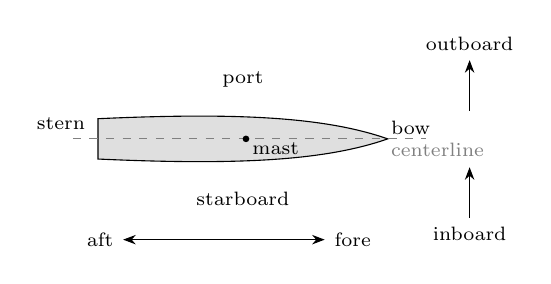
\begin{tikzpicture}[scale=0.8, every node/.style={font=\scriptsize}]
  % hull
  \draw[fill=gray!25] (-2.0,0) -- (-2.0,0.32) .. controls (0.2,0.42) and (1.6,0.35) .. (2.6,0)
                       .. controls (1.6,-0.35) and (0.2,-0.42) .. (-2.0,-0.32) -- cycle;
  \draw[dashed,gray] (-2.4,0) -- (3.2,0);
  \fill (0.35,0) circle (1.5pt);
  \node[anchor=north west,inner sep=1pt] at (0.4,0) {mast};
  \node[anchor=east] at (-2.05,0.25) {stern};
  \node[anchor=south west,inner sep=1pt] at (2.6,0.02) {bow};
  \node at (0.3,0.95) {port};
  \node at (0.3,-0.95) {starboard};
  \node[gray,anchor=north west,inner sep=1pt] at (2.6,-0.02) {centerline};
  % direction arrows
  \draw[{Stealth[length=1.6mm]}-{Stealth[length=1.6mm]}] (-1.6,-1.6) -- (1.6,-1.6);
  \node[anchor=east] at (-1.6,-1.6) {aft};
  \node[anchor=west] at (1.6,-1.6) {fore};
  \draw[-{Stealth[length=1.6mm]}] (3.9,0.45) -- (3.9,1.25) node[above] {outboard};
  \draw[-{Stealth[length=1.6mm]}] (3.9,-1.25) -- (3.9,-0.45);
  \node[anchor=north] at (3.9,-1.25) {inboard};
\end{tikzpicture}}

\subfloat[]{%
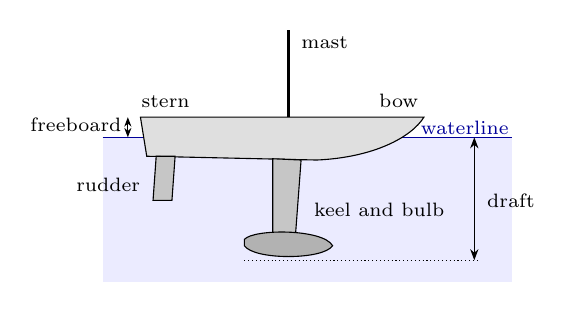
\begin{tikzpicture}[scale=0.8, every node/.style={font=\scriptsize}]
  % water
  \fill[blue!8] (-2.6,-2.3) rectangle (3.9,0);
  \draw[blue!60!black] (-2.6,0) -- (3.9,0) node[anchor=south east,inner sep=1pt] {waterline};
  % hull profile
  \draw[fill=gray!25] (-2.0,0.32) -- (2.5,0.32) .. controls (2.3,0.0) and (1.7,-0.32) .. (0.8,-0.36)
                       -- (-1.9,-0.3) -- cycle;
  % keel and bulb
  \draw[fill=gray!45] (0.1,-0.34) -- (0.55,-0.36) -- (0.45,-1.7) -- (0.1,-1.7) -- cycle;
  \draw[fill=gray!60] (-0.35,-1.62) .. controls (-0.2,-1.45) and (0.9,-1.45) .. (1.05,-1.72)
                       .. controls (0.9,-1.95) and (-0.2,-1.95) .. (-0.35,-1.72) -- cycle;
  \node[anchor=west] at (0.6,-1.15) {keel and bulb};
  % rudder
  \draw[fill=gray!45] (-1.75,-0.3) -- (-1.45,-0.3) -- (-1.5,-1.0) -- (-1.8,-1.0) -- cycle;
  \node[anchor=east] at (-1.85,-0.75) {rudder};
  % mast
  \draw[thick] (0.35,0.32) -- (0.35,1.7);
  \node[anchor=west] at (0.4,1.5) {mast};
  % freeboard and draft
  \draw[{Stealth[length=1.2mm]}-{Stealth[length=1.2mm]}] (-2.2,0) -- (-2.2,0.32);
  \node[anchor=east,inner sep=1pt] at (-2.25,0.2) {freeboard};
  \draw[{Stealth[length=1.4mm]}-{Stealth[length=1.4mm]}] (3.3,0) -- (3.3,-1.95);
  \draw[densely dotted] (-0.35,-1.95) -- (3.4,-1.95);
  \node[anchor=west] at (3.35,-1.0) {draft};
  \node[anchor=south] at (-1.6,0.32) {stern};
  \node[anchor=south] at (2.1,0.32) {bow};
\end{tikzpicture}}
\caption{Vessel terminology on ALAN's layout (schematic, not to scale).
(a) Top view of the hull with the fore--aft and inboard--outboard
directions. Port is on the left when facing the bow.
(b) Side view: freeboard and draft are measured from the waterline; the fin
keel and bulb sit below the mast, and the spade rudder at the stern.}
\label{fig:anatomy}
\end{figure}

\subsection{Physics of Sailing}
A sailboat is propelled by two opposing lift forces~\cite{skene2001}. Wind
flowing past the sail produces lift perpendicular to the apparent wind, and
on most headings this force points largely sideways. The keel, moving
through the water at a small leeway angle, produces a second lift force that
opposes the sideways component. What remains is a forward drive force, as
shown in Fig.~\ref{fig:physics}(b).

Because of this two-force balance, both the \emph{point of sail} (the boat's
heading relative to the wind) and the sail's \emph{angle of attack} (the angle
between the wing chord and the apparent wind) determine boat speed. A boat
cannot make headway within roughly \SI{45}{\degree} of the true wind on either
side; this \SI{90}{\degree} sector is called \emph{in irons} or the
\emph{no-go zone} (Fig.~\ref{fig:physics}(a)). To reach a target inside the
no-go zone, the boat must \emph{tack}, sailing a zig-zag course at the edge of
the zone.

The rudder acts as a second, smaller foil at the stern. Turning it toward
the wind reduces the effective keel force aft and turns the bow away from the
wind; turning it away from the wind does the opposite. The point at which the
sail force acts is the \emph{center of effort} (COE), and the point at which the
keel force acts is the \emph{center of lateral resistance} (CLR). Placing the
COE slightly aft of the CLR gives a mild \emph{weather helm}: the boat tends to
turn into the wind and depower if left uncontrolled, which is a safe default
for an autonomous vessel.

\begin{figure}[!t]
\centering
\subfloat[]{%
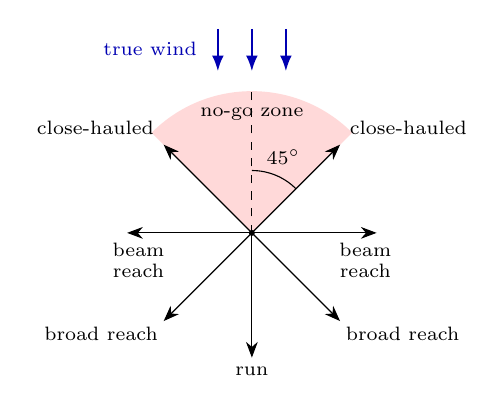
\begin{tikzpicture}[scale=0.72, every node/.style={font=\scriptsize}]
  % no-go zone
  \fill[red!15] (0,0) -- (45:2.5) arc (45:135:2.5) -- cycle;
  \node at (90:2.1) {no-go zone};
  % wind
  \foreach \x in {-0.6,0,0.6}
    \draw[-{Latex[length=2mm]},thick,blue!70!black] (\x,3.6) -- (\x,2.85);
  \node[blue!70!black,anchor=east] at (-0.8,3.25) {true wind};
  % headings
  \foreach \a/\lab/\anc in {45/close-hauled/west, 135/close-hauled/east,
                            0/beam reach/north, 180/beam reach/north,
                            -45/broad reach/north, -135/broad reach/north,
                            -90/run/north}
    \draw[-{Stealth[length=2mm]}] (0,0) -- (\a:2.2);
  \node[anchor=south west] at (45:2.2) {close-hauled};
  \node[anchor=south east] at (135:2.2) {close-hauled};
  \node[anchor=north] at (0:2.0) {\shortstack{beam\\reach}};
  \node[anchor=north] at (180:2.0) {\shortstack{beam\\reach}};
  \node[anchor=north west] at (-45:2.1) {broad reach};
  \node[anchor=north east] at (-135:2.1) {broad reach};
  \node[anchor=north] at (-90:2.2) {run};
  \draw[dashed] (0,0) -- (90:2.5);
  \draw (90:1.1) arc (90:45:1.1); \node at (67.5:1.45) {$45^\circ$};
  \fill (0,0) circle (1.5pt);
\end{tikzpicture}}
\hfil
\subfloat[]{%
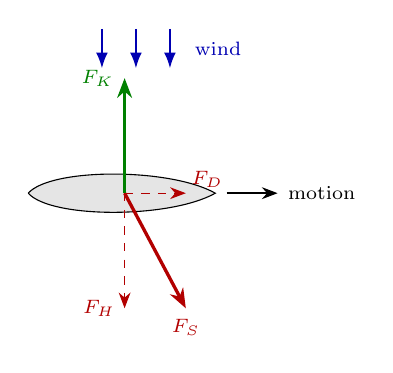
\begin{tikzpicture}[scale=0.72, every node/.style={font=\scriptsize}]
  % hull, heading +x
  \draw[fill=gray!20] (-1.6,0) .. controls (-1.2,0.45) and (0.9,0.45) .. (1.7,0)
                       .. controls (0.9,-0.45) and (-1.2,-0.45) .. (-1.6,0);
  \foreach \x in {-0.6,0,0.6}
    \draw[-{Latex[length=2mm]},thick,blue!70!black] (\x+0.3,2.9) -- (\x+0.3,2.2);
  \node[blue!70!black] at (1.75,2.55) {wind};
  % sail force (lift)
  \coordinate (C) at (0.1,0);
  \draw[-{Stealth[length=2.5mm]},very thick,red!70!black] (C) -- ++(-62:2.3) node[below] {$F_S$};
  % components
  \draw[-{Stealth[length=2mm]},dashed,red!70!black] (C) -- ++(1.08,0) node[above right=-2pt] {$F_D$};
  \draw[-{Stealth[length=2mm]},dashed,red!70!black] (C) -- ++(0,-2.03) node[left] {$F_H$};
  % keel force
  \draw[-{Stealth[length=2.5mm]},very thick,green!50!black] (C) -- ++(0,2.03) node[left] {$F_K$};
  \draw[-{Stealth[length=2mm]},thick] (1.9,0) -- (2.8,0) node[right] {motion};
\end{tikzpicture}}
\caption{Sailing fundamentals. (a) Points of sail; headings within
\SI{45}{\degree} of the true wind are not sailable. (b) Force balance seen from
above: the sail force $F_S$ splits into a drive component $F_D$ and a heeling
component $F_H$, which the keel force $F_K$ cancels.}
\label{fig:physics}
\end{figure}

\subsection{Hull, Keel, and Rudder Options}
Hulls are broadly \emph{displacement} or \emph{planing}. Displacement hulls
are rounder and deeper and float by displacing water; they are slower but
more stable. Planing hulls are flatter and rise onto the surface at speed;
they are faster but less stable~\cite{skene2001}. Keels are either
\emph{full}, running the length of the hull with shallow draft and high drag,
or \emph{fin}, a thin deep plate that is more efficient but increases
draft~\cite{sailingcats}. Rudders are classified by balance: a fully balanced
rudder pivots about its center of pressure and is easy to turn but does not
self-center, while an unbalanced rudder pivots at its leading edge, needs more
torque, and returns to center on its own~\cite{noahrudder}. A \emph{spade}
rudder hangs from its stock alone; a \emph{skeg} rudder is additionally
supported by a fin bolted to the hull.

\subsection{Wingsail Control Strategies}
Cloth sails are inexpensive but wear quickly. Rigid sails made of foam,
plastic, or composite are more durable and generate lift more efficiently,
which is why most autonomous sailboats use them~\cite{silva2019,sun2025}.
Three control strategies exist for rigid wingsails~\cite{sun2025}, compared
in Table~\ref{tab:sailtypes}. A \emph{traditional} wingsail is rotated
directly by a motor at the mast, which is simple but requires enough torque
to turn and hold the whole wing. A \emph{flap} wingsail adds a hinged trailing
flap; the motor moves only the flap, and the aerodynamic force on the flap
rotates the wing. A \emph{self-trimming} wingsail carries a tail roughly one
third the size of the main wing on a boom aft of the pivot. The motor turns
only the tail, whose aerodynamic moment rotates the wing to an equilibrium
angle of attack~\cite{elkaim2008,sailwings}. Actuation power is lowest for
the self-trimming design, at the cost of an indirect, delayed response that is
harder to control.

\begin{table}[!t]
\caption{Comparison of Rigid Wingsail Control Strategies}
\label{tab:sailtypes}
\centering
\begin{tabular}{@{}lccc@{}}
\toprule
 & Traditional & Flap & Self-trimming \\
\midrule
Actuated surface    & Whole wing & Flap & Tail \\
Actuator power      & High       & Medium & Low \\
Control complexity  & Low        & Medium & High \\
Response to command & Direct     & Indirect & Indirect, delayed \\
\bottomrule
\end{tabular}
\end{table}

\section{Related Work}
\label{sec:related}

Autonomous sailing has been an active research area for over a decade.
Stelzer's dissertation on autonomous sailboat navigation set foundational
algorithms for waypoint tracking and tacking under varying wind
conditions~\cite{stelzer2012}. From that research, the team found that a
state-machine approach to points of sail is most efficient in open water; his
earlier short-course routing method with Pr\"oll~\cite{stelzer2008} is the
basis for the tacking logic in Section~\ref{sec:sw}.

Commercial companies such as Saildrone have validated the viability of
autonomous wind-driven vessels for long-endurance ocean monitoring, using
rigid wingsail designs similar to ALAN's~\cite{saildrone,meinig2019}.

Furthermore, Sun \emph{et al.} provide a comprehensive review of autonomous
sailboat sail designs, concluding that rigid wingsails consistently
outperform cloth sails in autonomous applications due to their repeatability,
durability, and ability to be precisely controlled with low-power
actuators~\cite{sun2025}. Silva \emph{et al.} survey rigid-wing sailboats in
academia and industry~\cite{silva2019}, and Elkaim's Atlantis project showed
that a free-rotating wing with an aft tail can be made passively stable and
used it for GPS-guided line following~\cite{elkaim2006,elkaim2008}. The
Sailwings project documents practical mechanisms for driving the tail of a
self-trimming wingsail~\cite{sailwings}.

Also, Skene's foundational work on yacht design informs ALAN's hull geometry
decisions, particularly the relationship between center of effort and center
of lateral resistance~\cite{skene2001}. Rudder sizing followed a marine
rudder guide~\cite{noahrudder}, and the choice of a fixed fin keel drew on a
comparison of keels and daggerboards~\cite{sailingcats}.

Current autonomous platforms are either expensive (Saildrone) or use
conventional cloth sails. ALAN addresses this gap by pairing a self-trimming
rigid wingsail with a ballasted displacement hull, built entirely from
accessible components and low-cost fabrication resources.
\section{System Overview}
\label{sec:overview}

\subsection{Requirements}
The proposal set the following requirements for the capstone vessel:
\begin{enumerate}
\item Accept an ordered list of GPS waypoints from an operator and sail
between them without human input, tacking when a leg lies in the no-go zone.
\item Allow manual remote control from the ground station as a fallback.
\item Report position, heading, wind, actuator states, and battery status to
the ground station over a long-range, low-power radio link.
\item Remain stable and watertight in the wind and chop of local reservoirs.
\item Minimize actuator power so that the design scales to long missions.
\end{enumerate}

\subsection{Architecture}
Fig.~\ref{fig:boat} shows the assembled vessel and Fig.~\ref{fig:block} its
electrical and software architecture. All computation runs on one
NUCLEO-H755ZI-Q development board. The STM32H755's Cortex-M7 core (CM7) reads
every sensor and runs planning, control, and mode logic under FreeRTOS, while
its Cortex-M4 core (CM4) runs only the LoRa radio. The two cores exchange
telemetry and commands through shared memory (Section~\ref{sec:sw}). The hull
carries two deck hatches: the forward hatch gives access to the mast step and
sail-angle encoder, and the aft hatch holds the electronics enclosure. The
wind vane and rudder servo are mounted on the aft deck and transom.
Table~\ref{tab:specs} lists the principal dimensions, taken from the computer-aided design (CAD) model unless noted.

\begin{figure*}[!t]
\centering
\subfloat[]{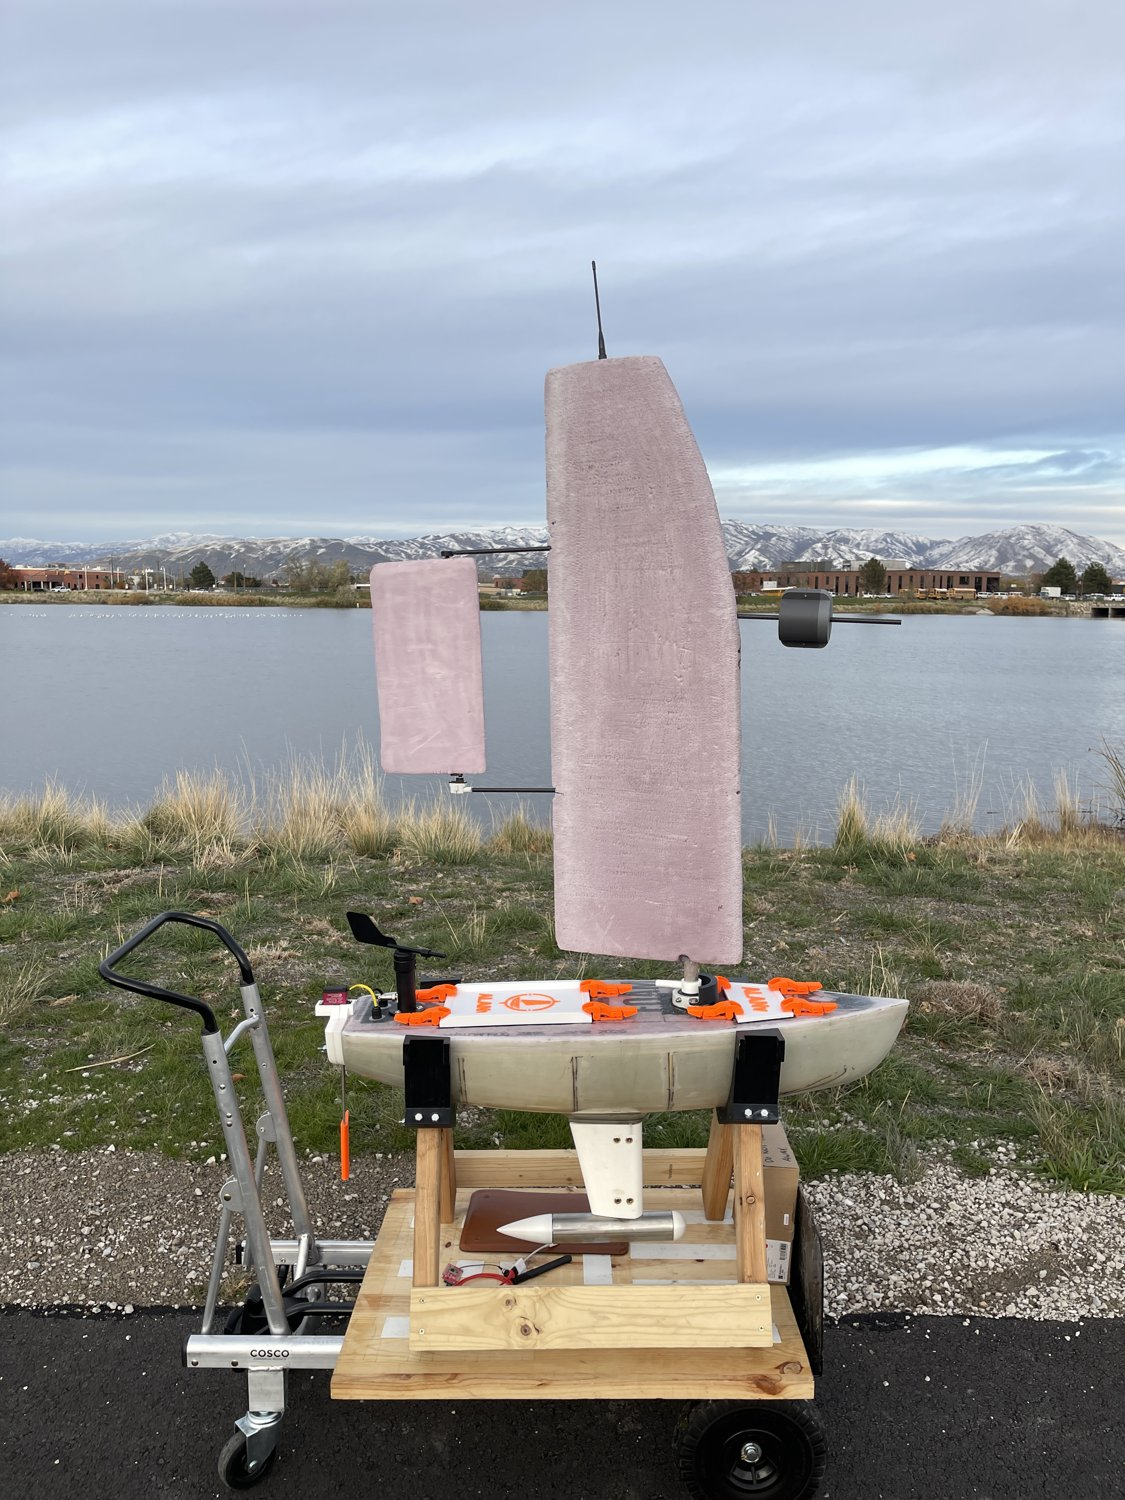
\includegraphics[height=5.6cm]{boat_full}}
\hfil
\subfloat[]{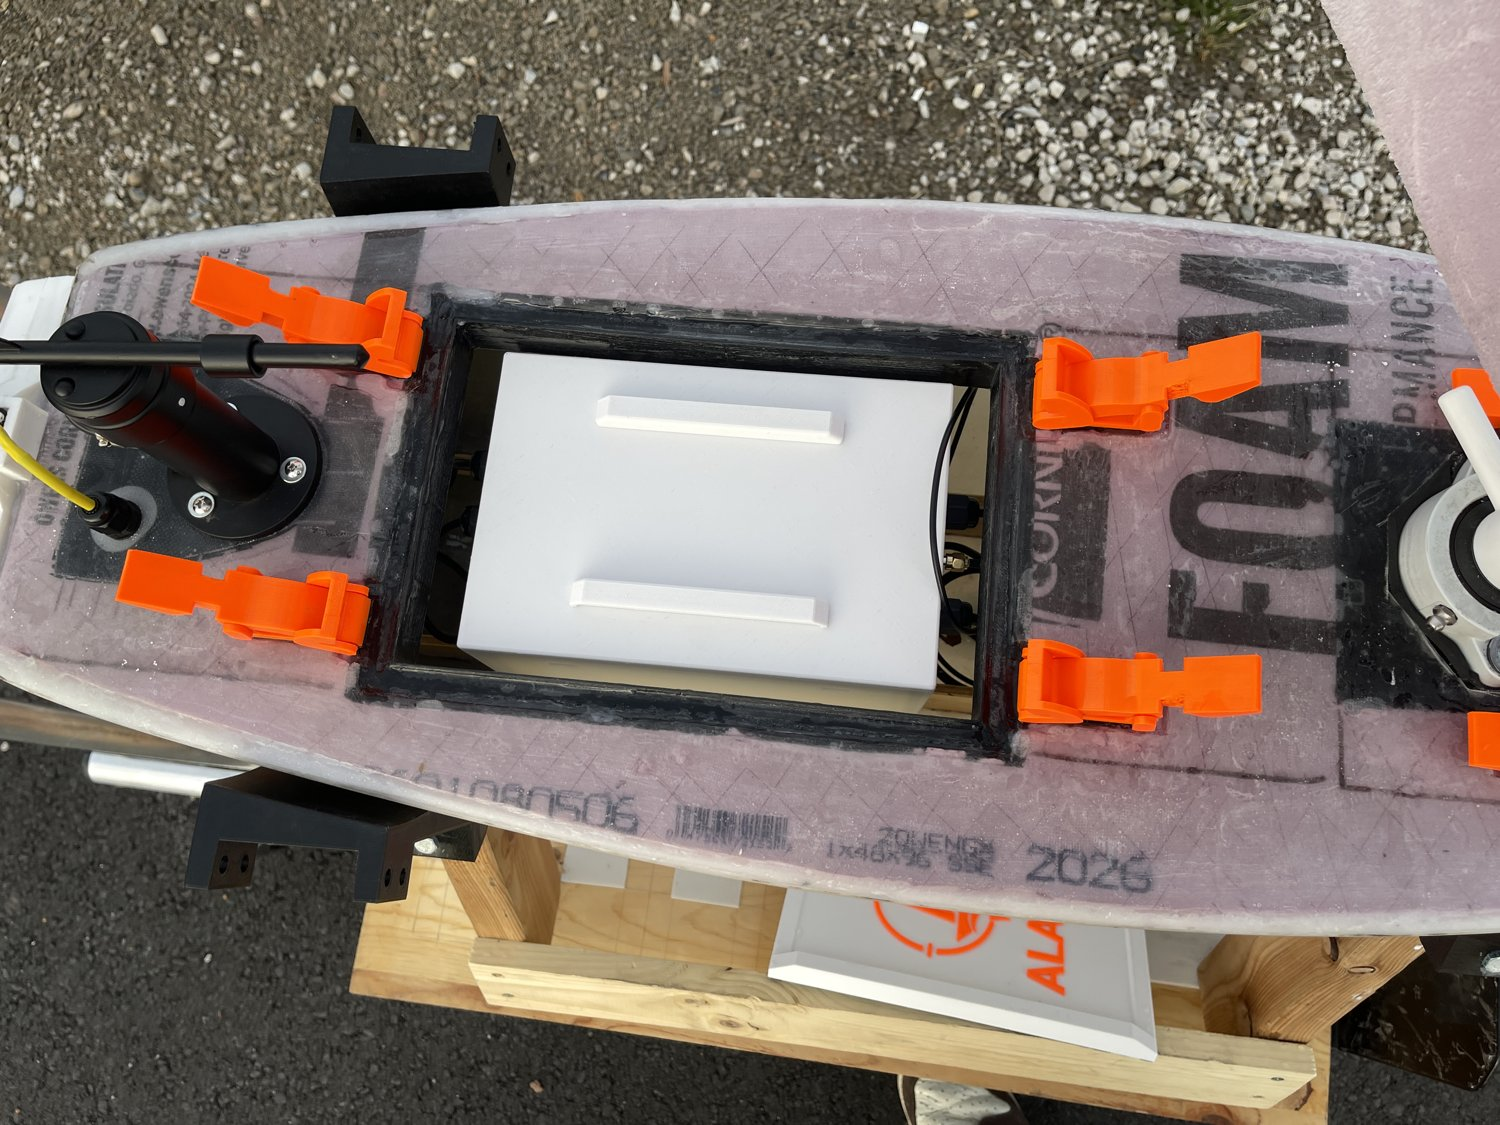
\includegraphics[height=5.6cm]{deck_top}}
\caption{ALAN at the test pond on November 18, 2026. (a) Side view: the
servo-driven tail, the main wing with the LoRa antenna at the masthead, and the
counterweight, with the fin keel and ballast bulb below the hull. (b) Aft deck
from above: the electronics enclosure in its hatch (cover removed), wind vane,
and printed hatch latches.}
\label{fig:boat}
\end{figure*}

\begin{table}[!t]
\caption{Principal Dimensions (from the CAD Model Unless Noted)}
\label{tab:specs}
\centering
\begin{tabular}{@{}lr@{}}
\toprule
Parameter & Value \\
\midrule
Length overall                 & \SI{1.00}{\meter} \\
Beam                           & \SI{0.31}{\meter} \\
Keel depth below hull          & \SI{0.23}{\meter} \\
Mass, ready to sail            & \SI{4.9}{\kilo\gram} (est.) \\
Ballast mass                   & 3.4 {kg} \\
Wing span $\times$ max.\ chord & 1.20 $\times$ \SI{0.35}{\meter} \\
Tail span $\times$ chord       & 0.43 $\times$ \SI{0.22}{\meter} \\
Wing rotation range            & $\pm\SI{90}{\degree}$ \\
Battery                        & \SI{14.8}{\volt} 4S lithium-polymer (LiPo), 1300 mAh \\
\bottomrule
\end{tabular}
\end{table}

\begin{figure*}[!t]
\centering
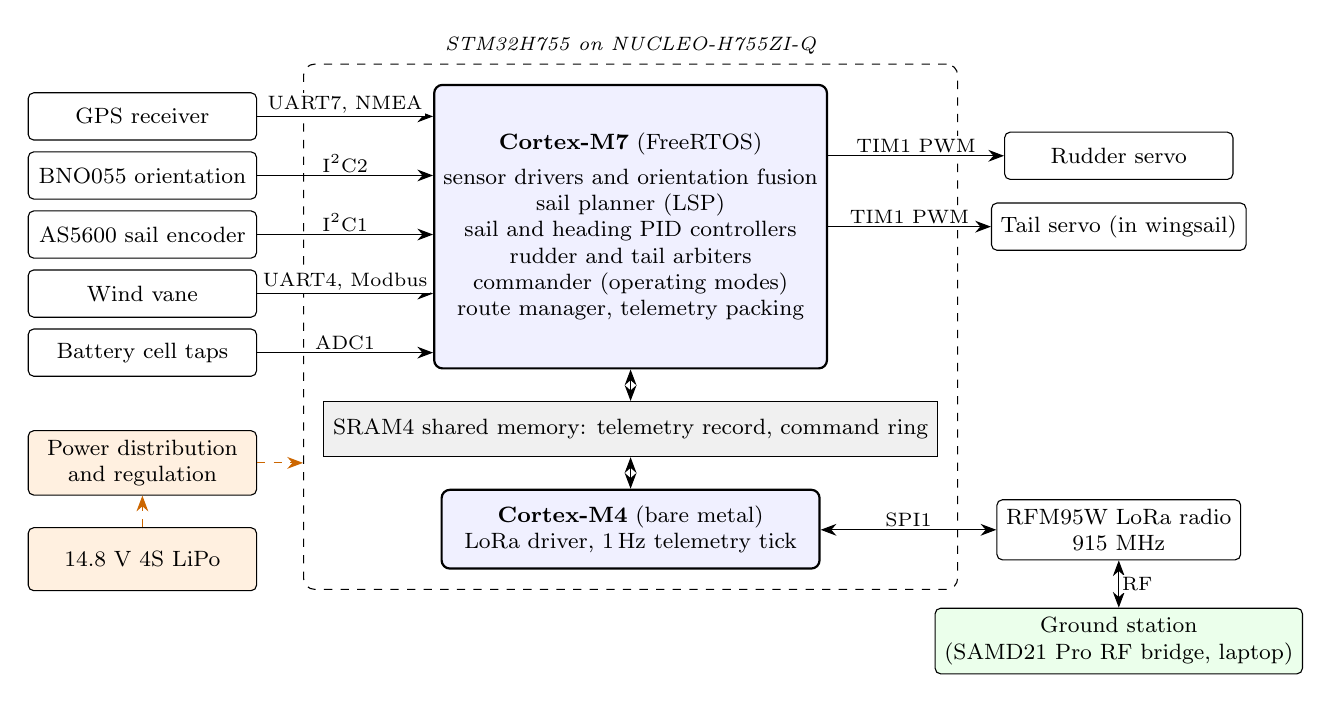
\begin{tikzpicture}[
  font=\footnotesize,
  blk/.style={draw, rounded corners=2pt, align=center, minimum height=6mm, minimum width=29mm, fill=white},
  core/.style={draw, thick, rounded corners=3pt, align=center, minimum width=48mm, fill=blue!6},
  pwr/.style={draw, rounded corners=2pt, align=center, minimum height=8mm, minimum width=29mm, fill=orange!12},
  data/.style={-{Stealth[length=2mm]}},
  power/.style={-{Stealth[length=2mm]}, orange!80!black, dashed},
  lbl/.style={font=\scriptsize, fill=white, inner sep=1pt}
]
\node[core, minimum height=36mm] (cm7) at (0,0) {\textbf{Cortex-M7} (FreeRTOS)\\[3pt]sensor drivers and orientation fusion\\sail planner (LSP)\\sail and heading PID controllers\\rudder and tail arbiters\\commander (operating modes)\\route manager, telemetry packing};
\node[draw, fill=gray!12, minimum width=48mm, minimum height=7mm, align=center, below=4mm of cm7] (sram) {SRAM4 shared memory: telemetry record, command ring};
\node[core, minimum height=10mm, below=4mm of sram] (cm4) {\textbf{Cortex-M4} (bare metal)\\LoRa driver, \SI{1}{\hertz} telemetry tick};
\begin{scope}[on background layer]
\node[draw, dashed, rounded corners=4pt, inner sep=2.5mm, fit=(cm7)(sram)(cm4),
      label={[font=\scriptsize\itshape, anchor=south]north:STM32H755 on NUCLEO-H755ZI-Q}] (mcu) {};
\end{scope}
\draw[{Stealth[length=2mm]}-{Stealth[length=2mm]}] (cm7) -- (sram);
\draw[{Stealth[length=2mm]}-{Stealth[length=2mm]}] (sram) -- (cm4);
% sensors
\node[blk] (gps)  at (-6.2, 1.40) {GPS receiver};
\node[blk] (imu)  at (-6.2, 0.65) {BNO055 orientation};
\node[blk] (enc)  at (-6.2,-0.10) {AS5600 sail encoder};
\node[blk] (wind) at (-6.2,-0.85) {Wind vane};
\node[blk] (taps) at (-6.2,-1.60) {Battery cell taps};
\draw[data] (gps.east)  -- node[lbl,above]{UART7, NMEA}  (gps.east  -| cm7.west);
\draw[data] (imu.east)  -- node[lbl,above]{I\textsuperscript{2}C2} (imu.east  -| cm7.west);
\draw[data] (enc.east)  -- node[lbl,above]{I\textsuperscript{2}C1} (enc.east  -| cm7.west);
\draw[data] (wind.east) -- node[lbl,above]{UART4, Modbus} (wind.east -| cm7.west);
\draw[data] (taps.east) -- node[lbl,above]{ADC1} (taps.east -| cm7.west);
% actuators
\node[blk] (rud)  at (6.2, 0.9) {Rudder servo};
\node[blk] (tail) at (6.2, 0.0) {Tail servo (in wingsail)};
\draw[data] (rud.west  -| cm7.east) -- node[lbl,above]{TIM1 PWM} (rud.west);
\draw[data] (tail.west -| cm7.east) -- node[lbl,above]{TIM1 PWM} (tail.west);
% radio and ground station
\node[blk] (lora) at (6.2, -3.85) {RFM95W LoRa radio\\915 MHz};
\node[blk, fill=green!8, below=6mm of lora] (gs) {Ground station\\(SAMD21 Pro RF bridge, laptop)};
\draw[{Stealth[length=2mm]}-{Stealth[length=2mm]}] (lora.west -| cm4.east) -- node[lbl,above]{SPI1} (lora.west);
\draw[{Stealth[length=2mm]}-{Stealth[length=2mm]}] (lora) -- node[lbl,right]{RF} (gs);
% power
\node[pwr] (pdb) at (-6.2,-3.0) {Power distribution\\and regulation};
\node[pwr, below=4mm of pdb] (bat) {14.8 V 4S LiPo};
\draw[power] (bat) -- (pdb);
\draw[power] (pdb.east) -- (pdb.east -| mcu.west);
\end{tikzpicture}
\caption{Electrical and software architecture. The CM7 owns all sensing,
control, and actuation; the CM4 owns the radio; the cores communicate only
through shared SRAM4. Solid arrows carry data and dashed arrows carry power.}
\label{fig:block}
\end{figure*}

\section{Mechanical Design and Fabrication}
\label{sec:mech}

The proposal specified a trimaran: a displacement main hull with two
outrigger floats (amas), a self-trimming wingsail, a bulbed fin keel, and a
spade rudder. The as-built ALAN is a monohull. On-water testing showed that
the monohull, with its ballasted fin keel providing the righting moment, was
stable enough for the calm reservoir conditions it was tested in, so the amas
were not included (Section~\ref{sec:integration}). The displacement hull was
chosen for stability, the self-trimming wingsail for its low actuation power,
the fin keel for manufacturability (hull and keel are built separately and
bolted together), the bulb for control over mass and center of gravity, and
the spade rudder because it is the easiest to modify and repair.
Fig.~\ref{fig:cad} shows the complete CAD model.
Table~\ref{tab:changes} summarizes where the as-built vessel departs from the
proposal; the reasons are given in the subsections below.

\begin{figure*}[!t]
\centering
\subfloat[]{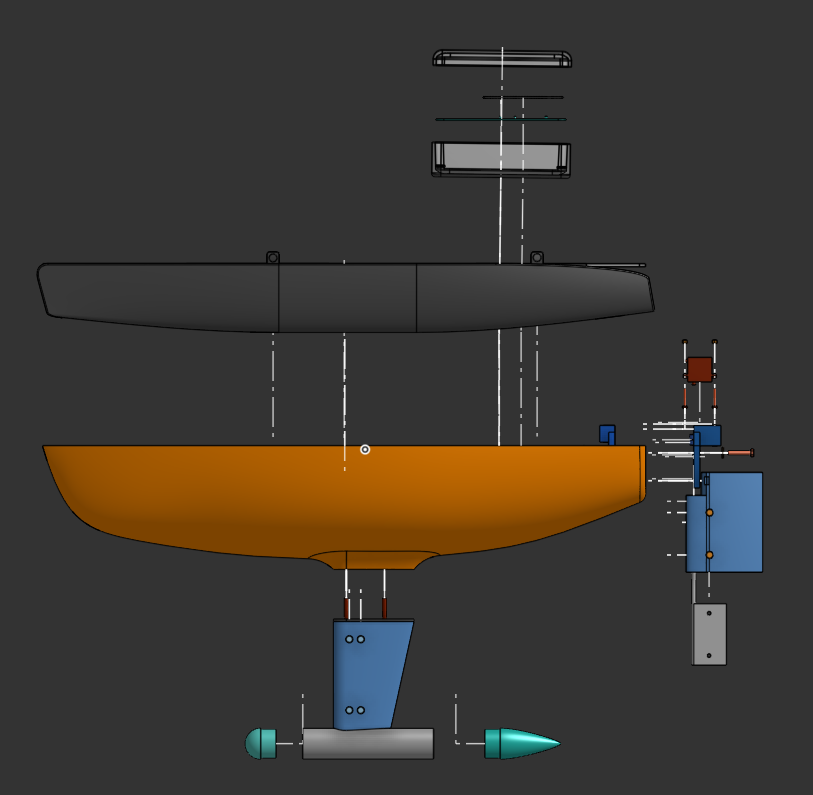
\includegraphics[height=5.2cm]{cad_side}}
\hfil
\subfloat[]{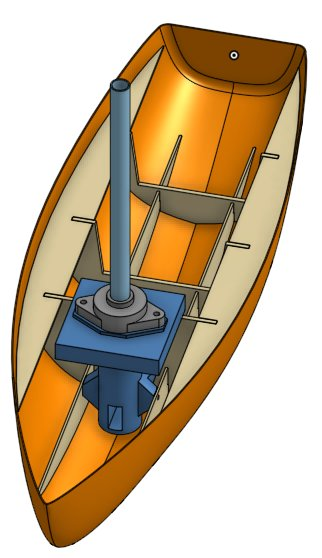
\includegraphics[height=5.2cm]{cad_interior}}
\caption{CAD model. (a) Exploded side view showing the hatch covers, deck, hull,
keel and bulb, and rudder assembly. (b) Hull interior with bulkheads and
the mast step.}
\label{fig:cad}
\end{figure*}

\begin{table*}[!t]
\caption{Changes from the ECE 3992 Proposal}
\label{tab:changes}
\centering
\begin{tabular}{@{}p{0.15\textwidth}p{0.33\textwidth}p{0.45\textwidth}@{}}
\toprule
Item & Proposed & As built \\
\midrule
Tail drive & Servo inside the wing, wire linkage to the tail & Servo at the tail's lower pivot, driving it directly; no linkage backlash \\
Wing skin & Fiberglass over carved XPS foam & Bare carved XPS foam; fiberglass skin planned for the final iteration \\
Mast & Hollow carbon fiber rod & \SI{3}{ft} 6061 aluminum tube in a flanged ball-bearing unit \\
Wing travel & Free rotation & Printed hard stops at $\pm\SI{90}{\degree}$ \\
Sail angle sensing & Estimated from servo position and IMU yaw & AS5600 magnetic encoder at the mast step \\
Ballast & Bulb tube filled with up to \SI{2}{\kilo\gram} of steel balls & Two removable threaded ballast canisters, adjustable at the dock \\
Keel finish & Carbon fiber or fiberglass wrap & Bare printed fairing \\
Electronics housing & Pelican M60 case & Printed enclosure in a sealed deck hatch with cable glands \\
Battery & 3S \SI{11.1}{\volt} LiPo with a battery management system (BMS) & 4S \SI{14.8}{\volt} LiPo with a BMS and per-cell voltage telemetry \\
Orientation & Complementary filter with GPS/IMU dead reckoning & BNO055 onboard nine-axis fusion, quaternion averaging, GPS surge speed \\
Failsafe & Return to home on link loss & SAFE mode and arbiter timeouts; link-loss timeout implemented but not yet enabled \\
Hull form & Trimaran (main hull with two amas) & Monohull; ballasted keel provides the righting moment \\
\bottomrule
\end{tabular}
\end{table*}

\subsection{Hull}
The hull is a wet layup of fiberglass and epoxy in a two-piece female mold.
The mold was 3D printed in polylactic acid (PLA) in bow and stern halves that bolt together
(Fig.~\ref{fig:hull}(a)), then surfaced with filler primer and a 2K gloss
topcoat, waxed, and coated with a polyvinyl alcohol (PVA) film release agent. Seven plies of \SI{4}{oz} plain-weave fiberglass
laid up with 5:1 marine epoxy give a cured wall thickness of about
\SI{1}{\milli\meter}. The keel mount was
reinforced with additional plies and a metal plate laminated inside the mount
boss; the transom received extra plies but a removable internal plate, so
that rudder hardware can be serviced. Bulkheads and the sail templates were
laser cut from plywood (Fig.~\ref{fig:hull}(b)) and bonded into the hull to
stiffen it and to locate the mast step.

The deck is extruded polystyrene (XPS) foam board laminated with fiberglass
and resin. Two printed hatch coamings are bonded into the deck, and each
hatch cover is held by four printed over-center latches
(Fig.~\ref{fig:deck}(a)). Cable penetrations use compression cable glands.

\begin{figure}[!t]
\centering
\subfloat[]{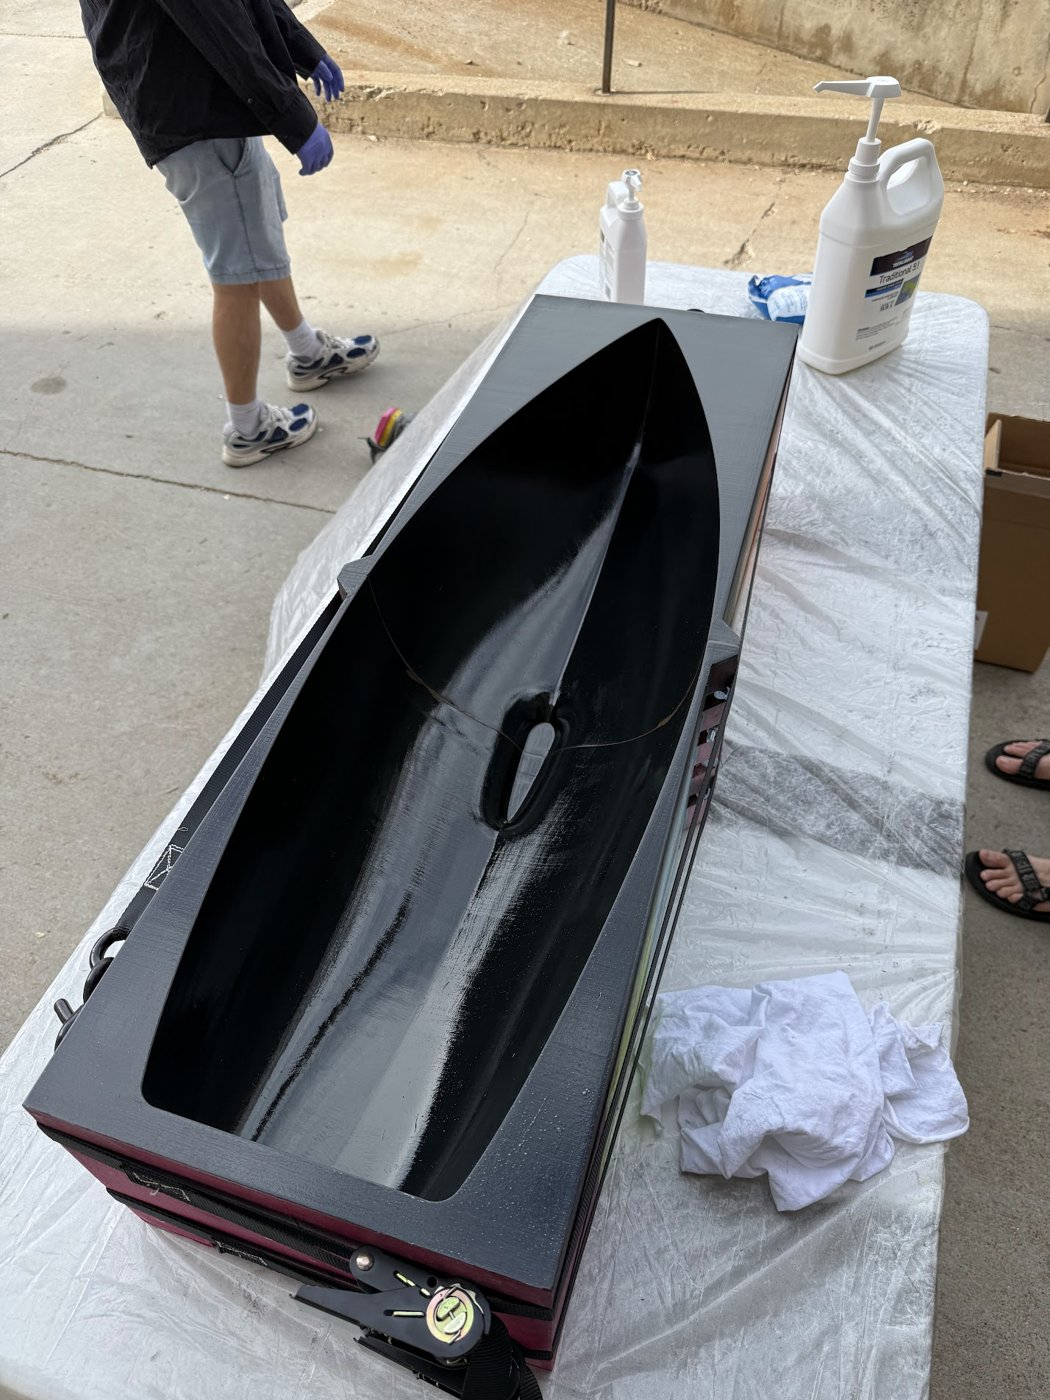
\includegraphics[height=4.4cm]{hull_mold}}
\hfil
\subfloat[]{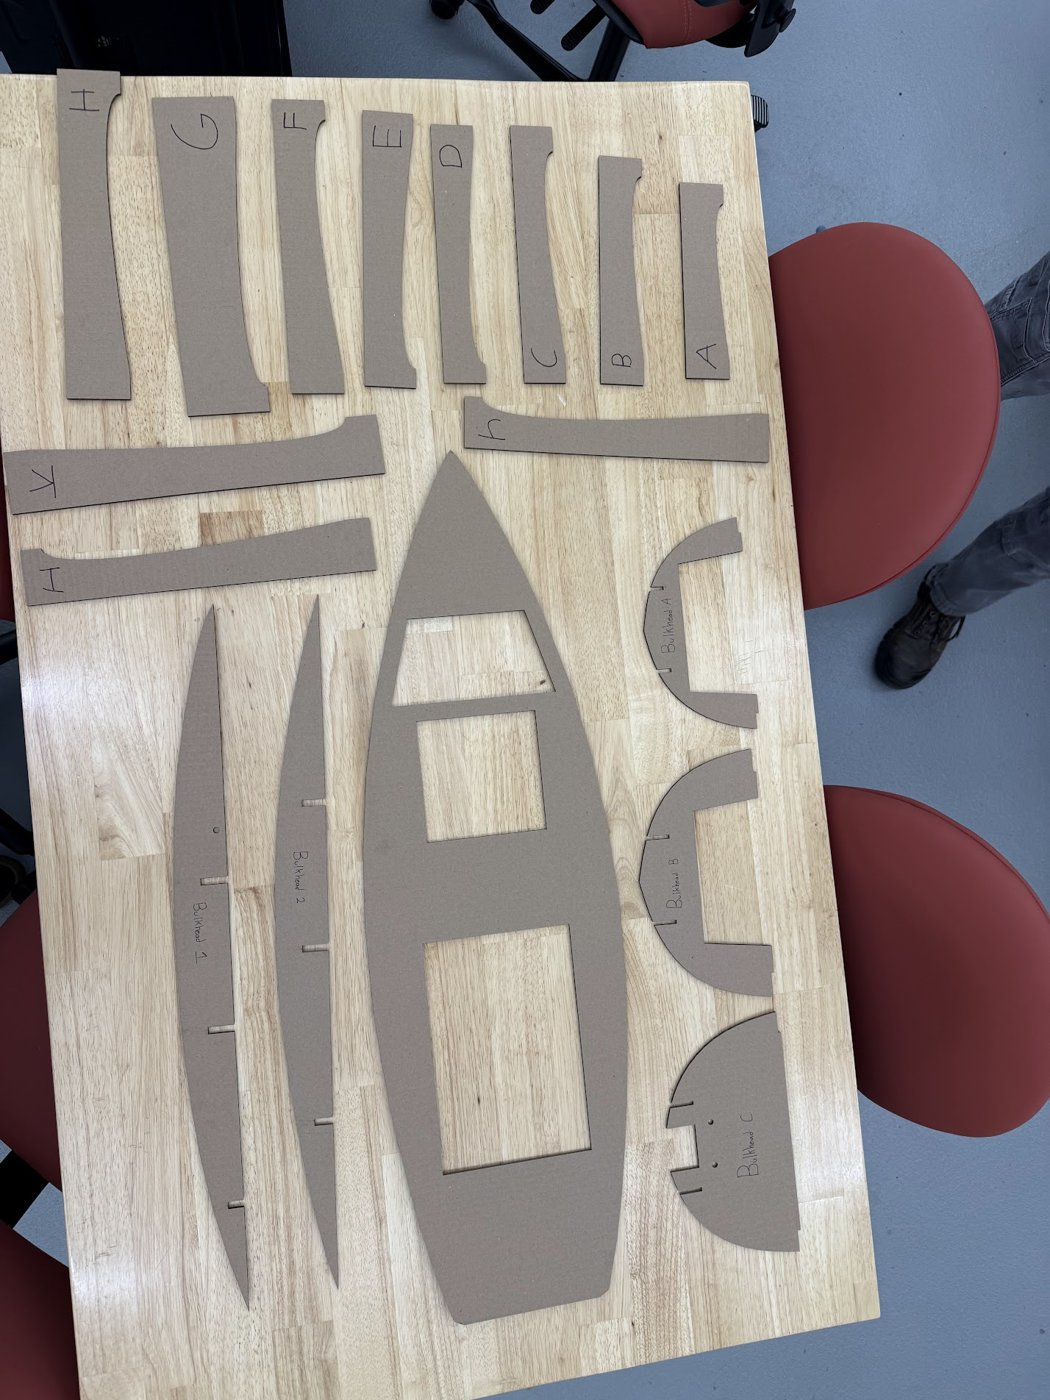
\includegraphics[height=4.4cm]{laser_cut}}
\caption{Hull fabrication. (a) Printed two-piece female mold prepared for the
fiberglass layup. (b) Laser-cut plywood bulkheads and sail templates.}
\label{fig:hull}
\end{figure}

\begin{figure}[!t]
\centering
\subfloat[]{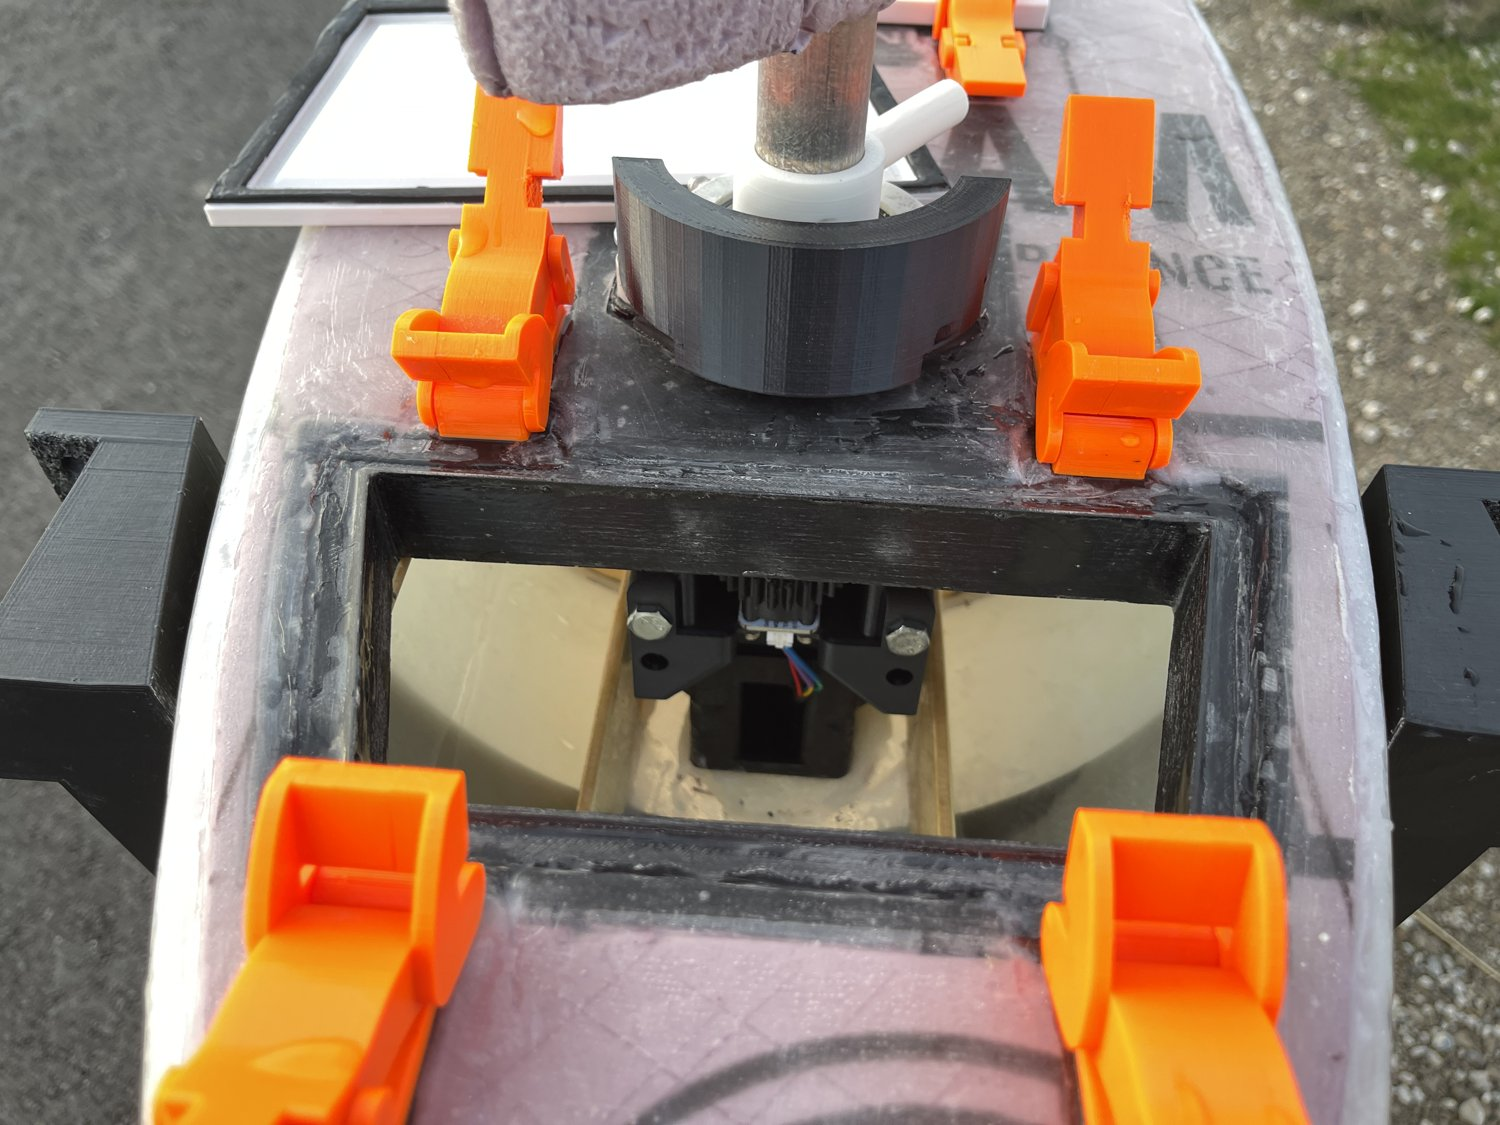
\includegraphics[height=3.9cm]{bow_deck}}
\hfil
\subfloat[]{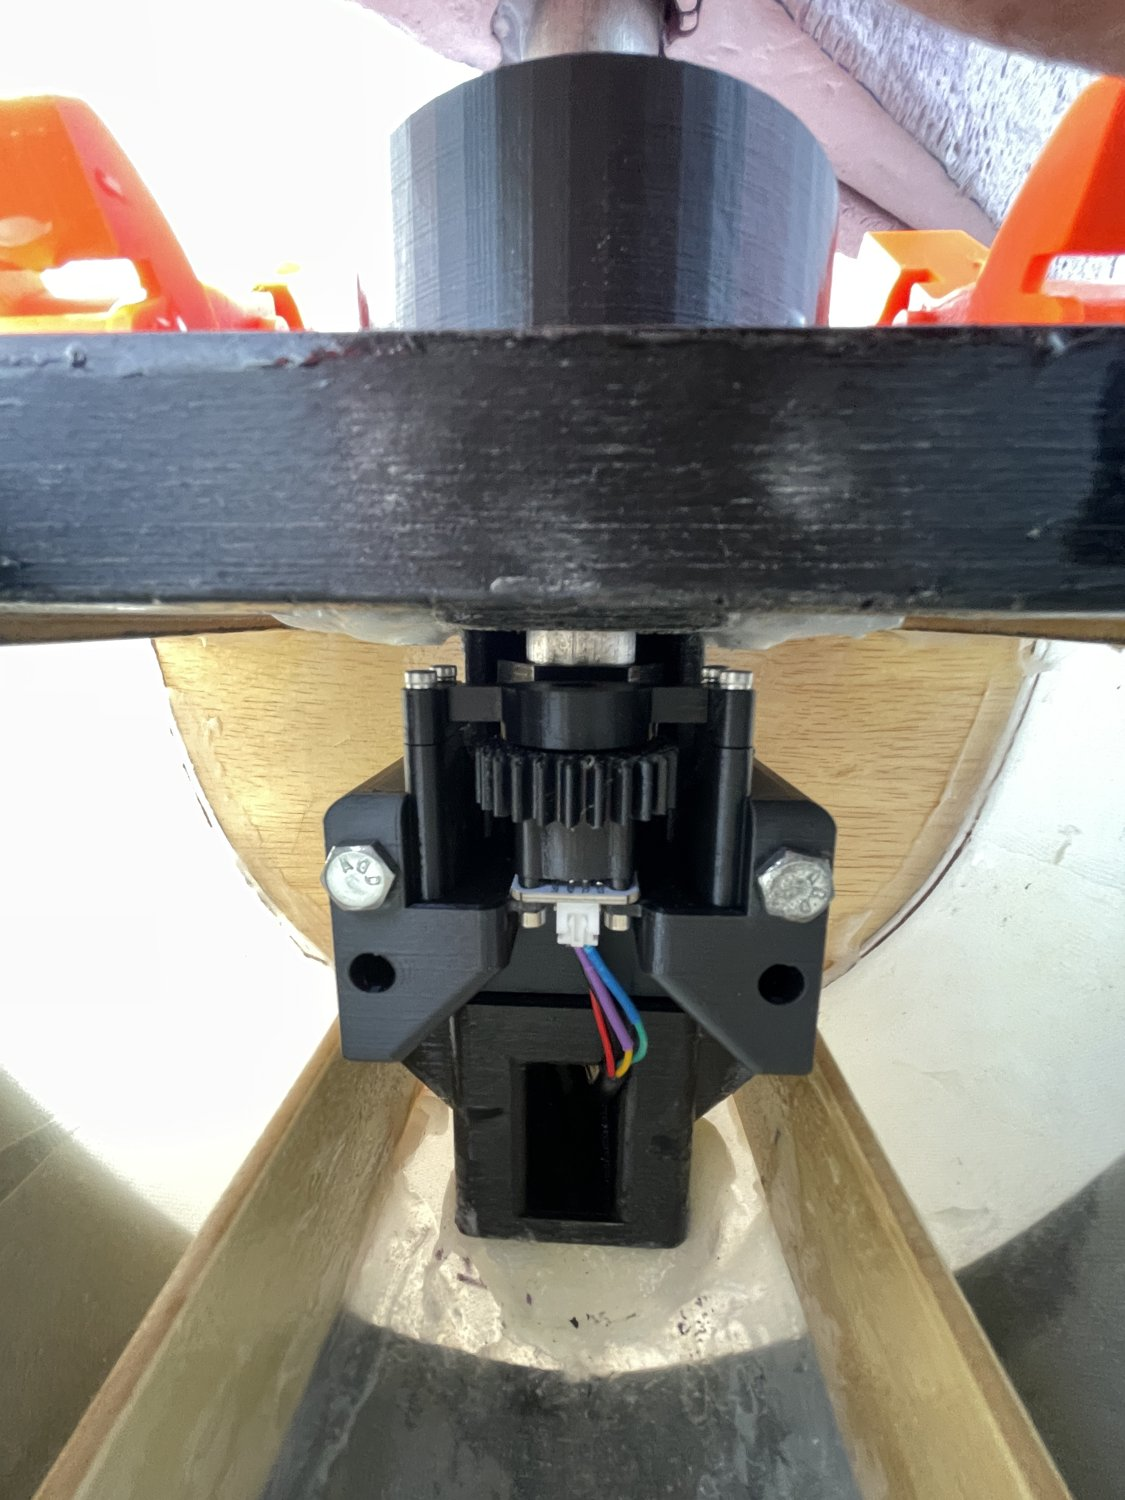
\includegraphics[height=3.9cm]{mast_encoder}}
\caption{Forward deck. (a) Mast base with its collar and guard ring, the
forward hatch open with the encoder assembly visible below, and the printed
over-center latches. (b) Below deck: spur gear and AS5600 magnetic encoder that measure the wing angle
relative to the hull.}
\label{fig:deck}
\end{figure}

\subsection{Keel and Ballast Bulb}
The keel has three parts: a frame, a fairing, and ballast
(Fig.~\ref{fig:keel}). The frame is 304 stainless steel, chosen for its
corrosion resistance: a \SI{0.25}{in} plate mounting bracket, a
\SI{0.5}{in} $\times$ \SI{7}{in} square-bar post, and a \SI{2}{in}
$\times$ \SI{8.5}{in} round tube that forms the core of the bulb. The bracket
bolts through the reinforced keel boss with 1/4-20 bolts and nylon-insert
lock nuts. Two mirrored printed PLA fairing halves clamp around the post with
four bolts and give the keel its foil
section, sized to place the CLR correctly relative to the sail's
COE~\cite{noahrudder,skene2001}.

The proposal called for filling the bulb tube with steel shot. Instead, the
ballast is carried in two stainless canisters that slide into the bulb tube
from either end and are retained by threaded studs
(Fig.~\ref{fig:keel}(c)). A rounded printed nose cap and a tapered tail cap
fair the ends. Because each canister can be loaded independently, the ballast
mass and its fore-aft position can be changed at the dock to trim the boat
without opening the keel. Rust streaks below the fairing bolts in
Fig.~\ref{fig:keel}(b) come from zinc-plated fasteners; these should be
replaced with stainless hardware before extended use in water.

\begin{figure}[!t]
\centering
\subfloat[]{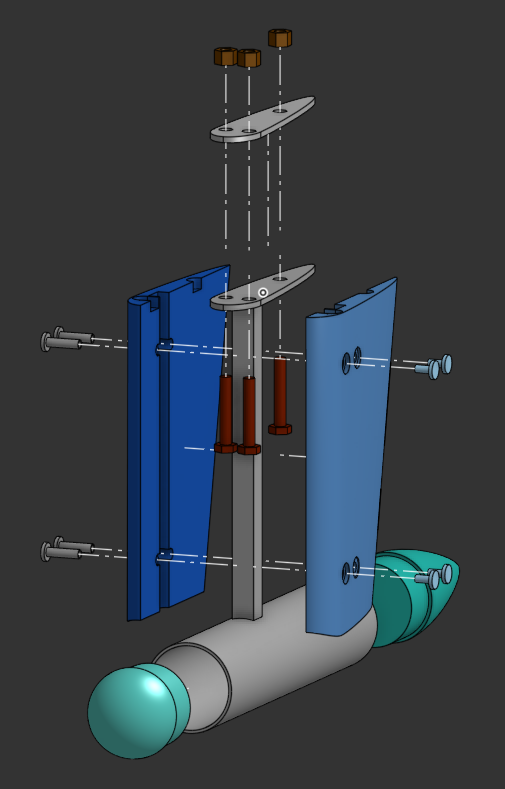
\includegraphics[height=3.0cm]{cad_keel}}
\hfil
\subfloat[]{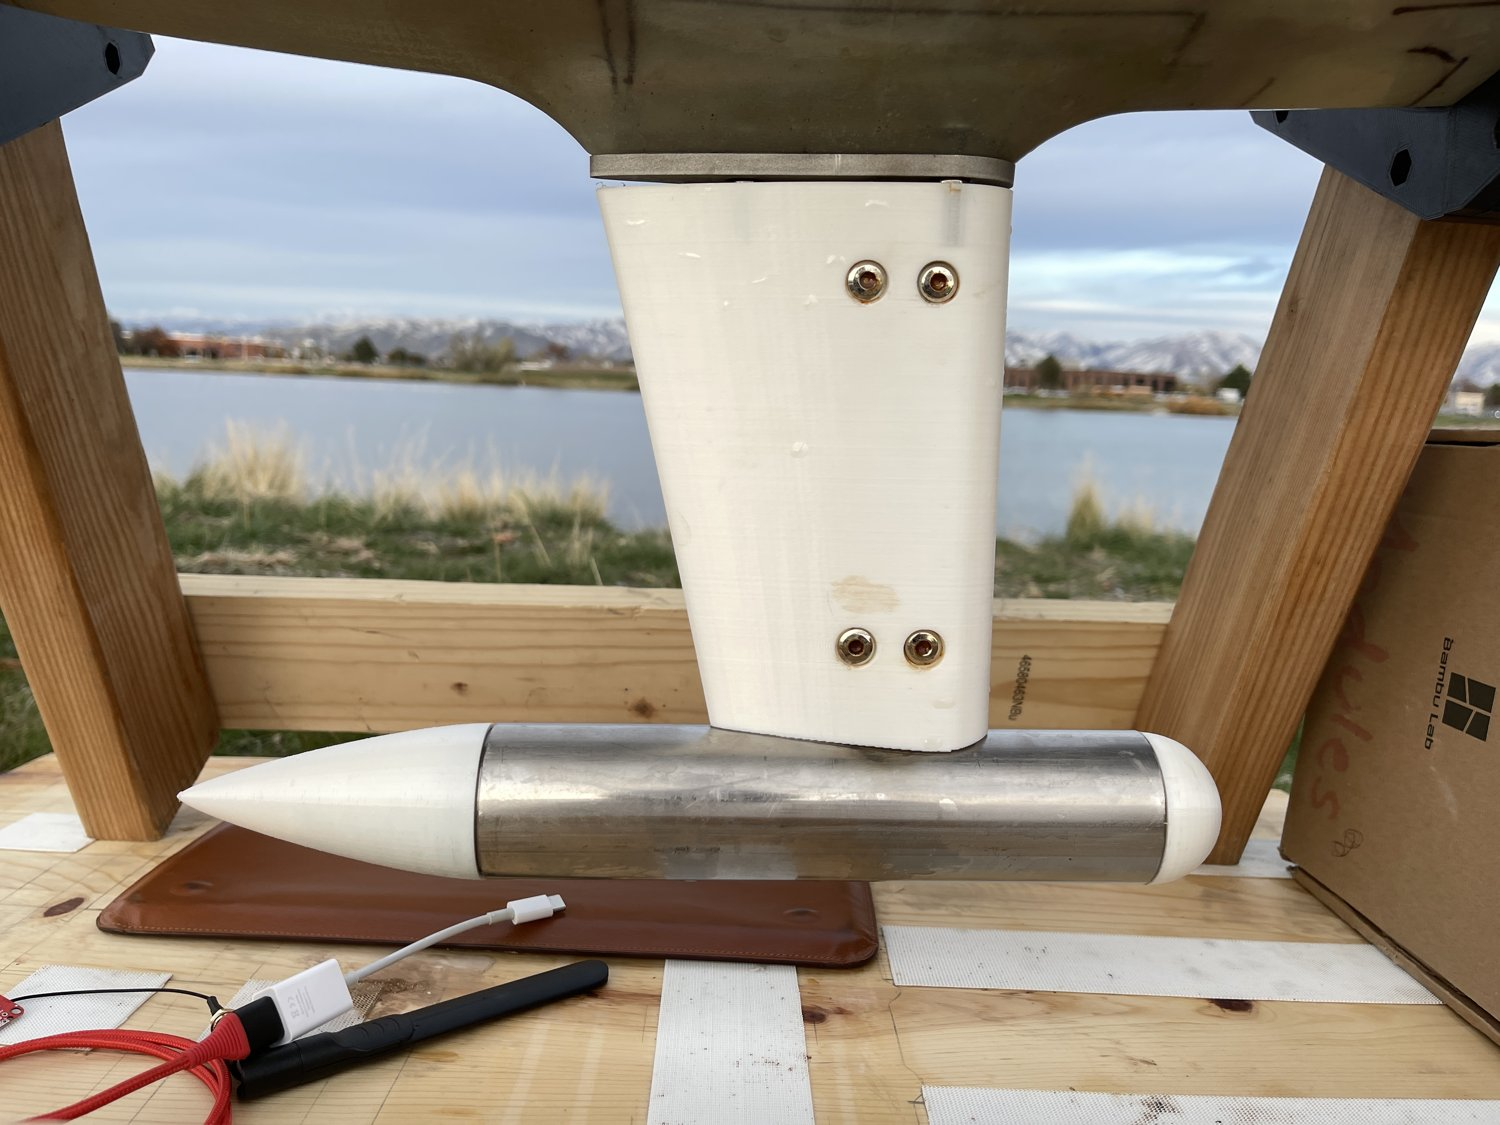
\includegraphics[height=3.0cm]{keel_bulb}}
\hfil
\subfloat[]{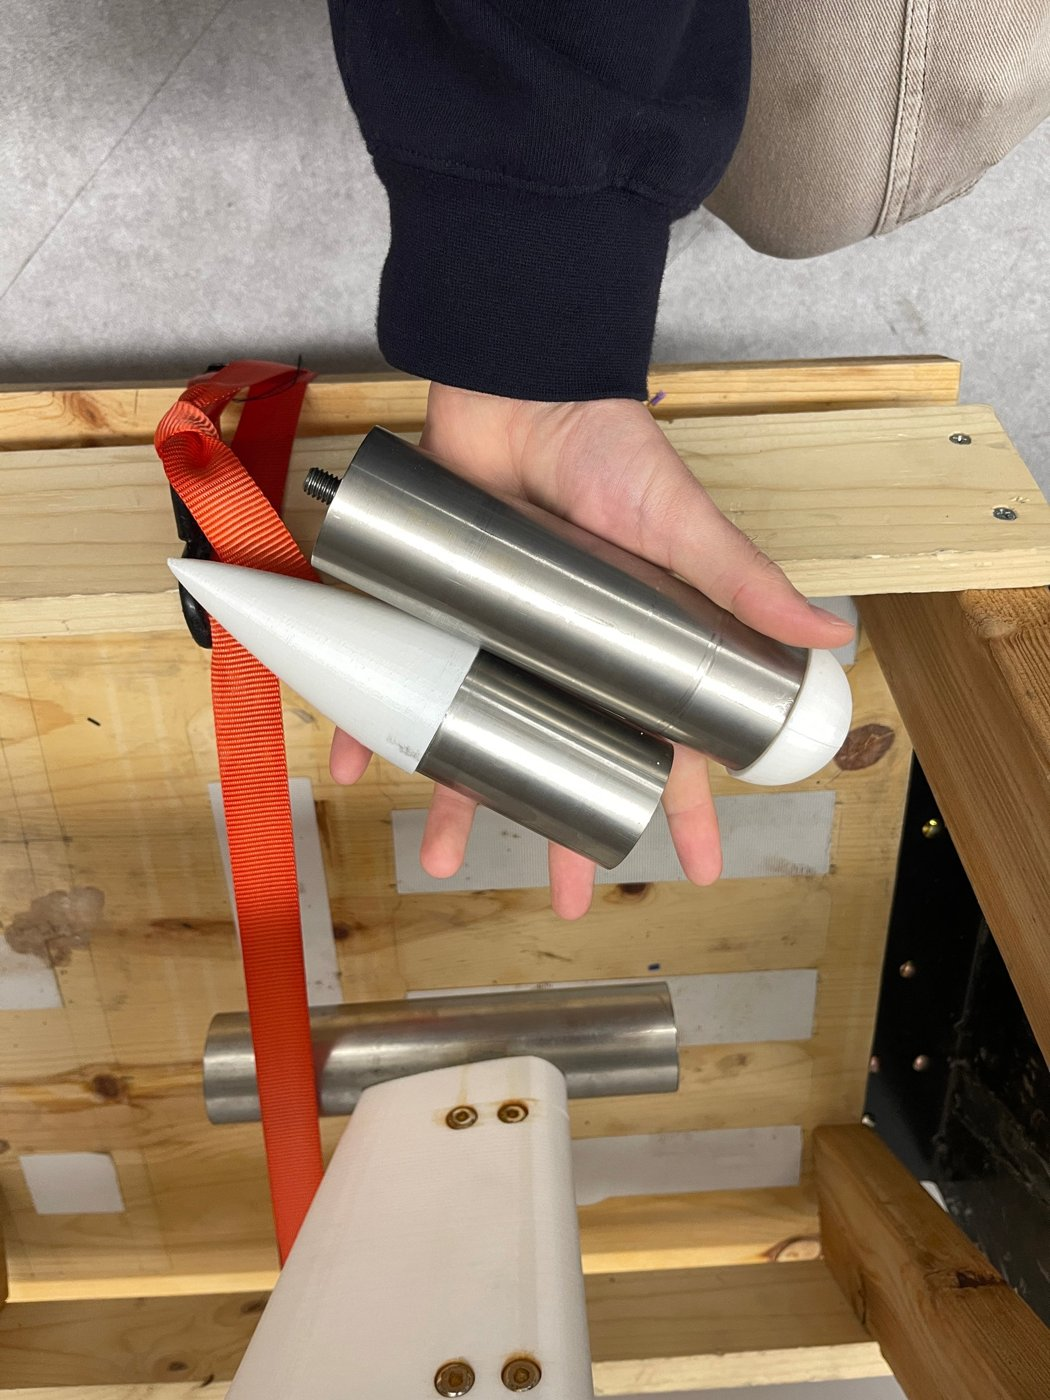
\includegraphics[height=3.0cm]{ballast_canisters}}
\caption{Keel. (a) Exploded CAD of the steel frame, fairing halves, and bulb.
(b) As built, with the fairing bolted to the post and the bulb caps fitted.
(c) Removable ballast canisters with their nose and tail caps.}
\label{fig:keel}
\end{figure}

\subsection{Rudder}
The spade rudder hangs from a \SI{0.25}{in} $\times$ \SI{12}{in} 304
stainless round-bar shaft. A printed rudder blade clamps around the shaft and
is pinned with a cross bolt and barrel nut, so blades of different area can
be swapped without disturbing the shaft. The shaft turns in two R188 ceramic
ball bearings, chosen for corrosion resistance, held in a two-part clamp. The
fore section of the clamp sits against the inside of the transom and the aft
section, with \SI{0.065}{in} aluminum mounting plates, clamps over it with
1/4-20 bolts and nylon-insert lock nuts, so the assembly can be
removed without cutting the hull (Fig.~\ref{fig:rudder}(a)). A DS3218MG
\SI{20}{kg\cdot cm} waterproof digital servo in a printed transom mount
drives the shaft through a 25-tooth spline to 1/4-in.\ bore coupler
(Fig.~\ref{fig:rudder}(b)); Fig.~\ref{fig:rudder}(c) shows the blade. In the
CAD model the blade has a \SI{70}{\milli\meter} chord and a
\SI{100}{\milli\meter} span, an area of \SI{70}{\centi\meter\squared}.

\begin{figure}[!t]
\centering
\subfloat[]{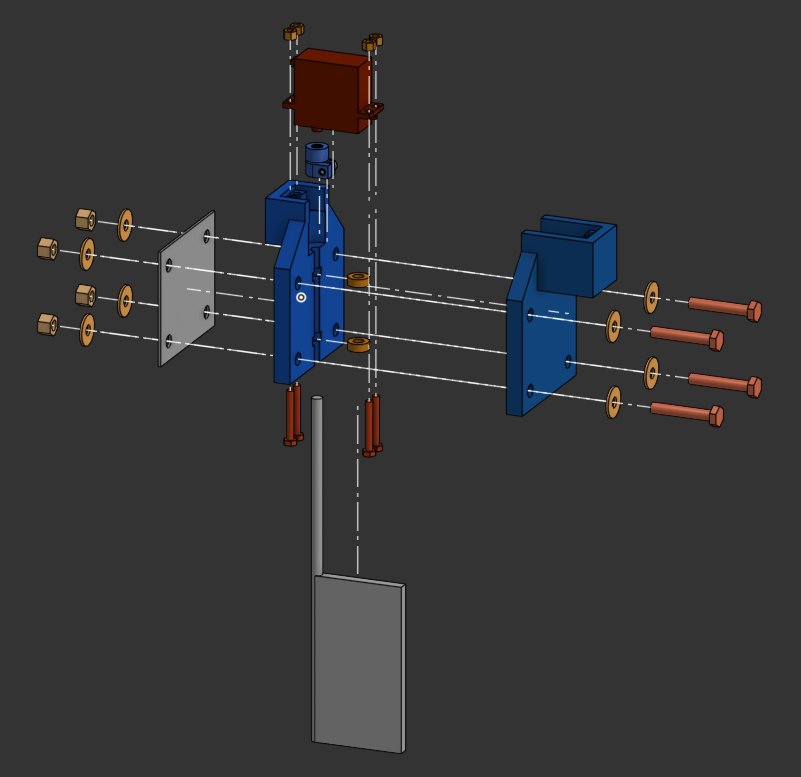
\includegraphics[height=3.2cm]{cad_rudder}}
\hfil
\subfloat[]{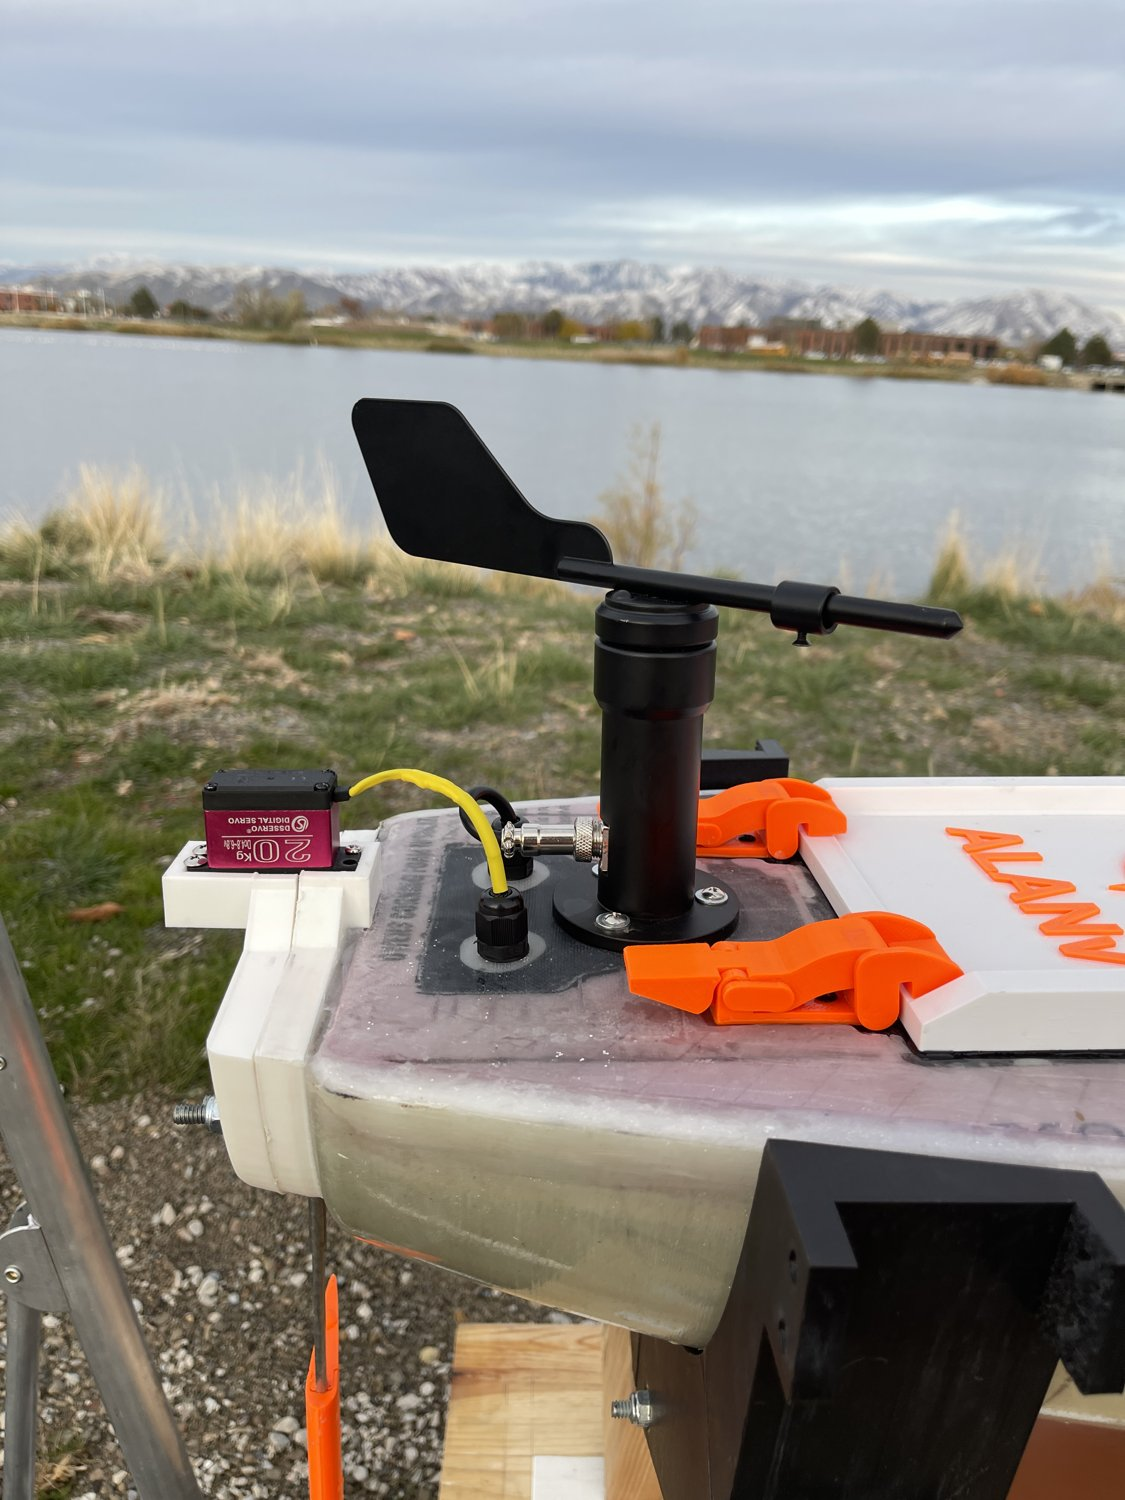
\includegraphics[height=3.2cm]{stern_deck}}
\hfil
\subfloat[]{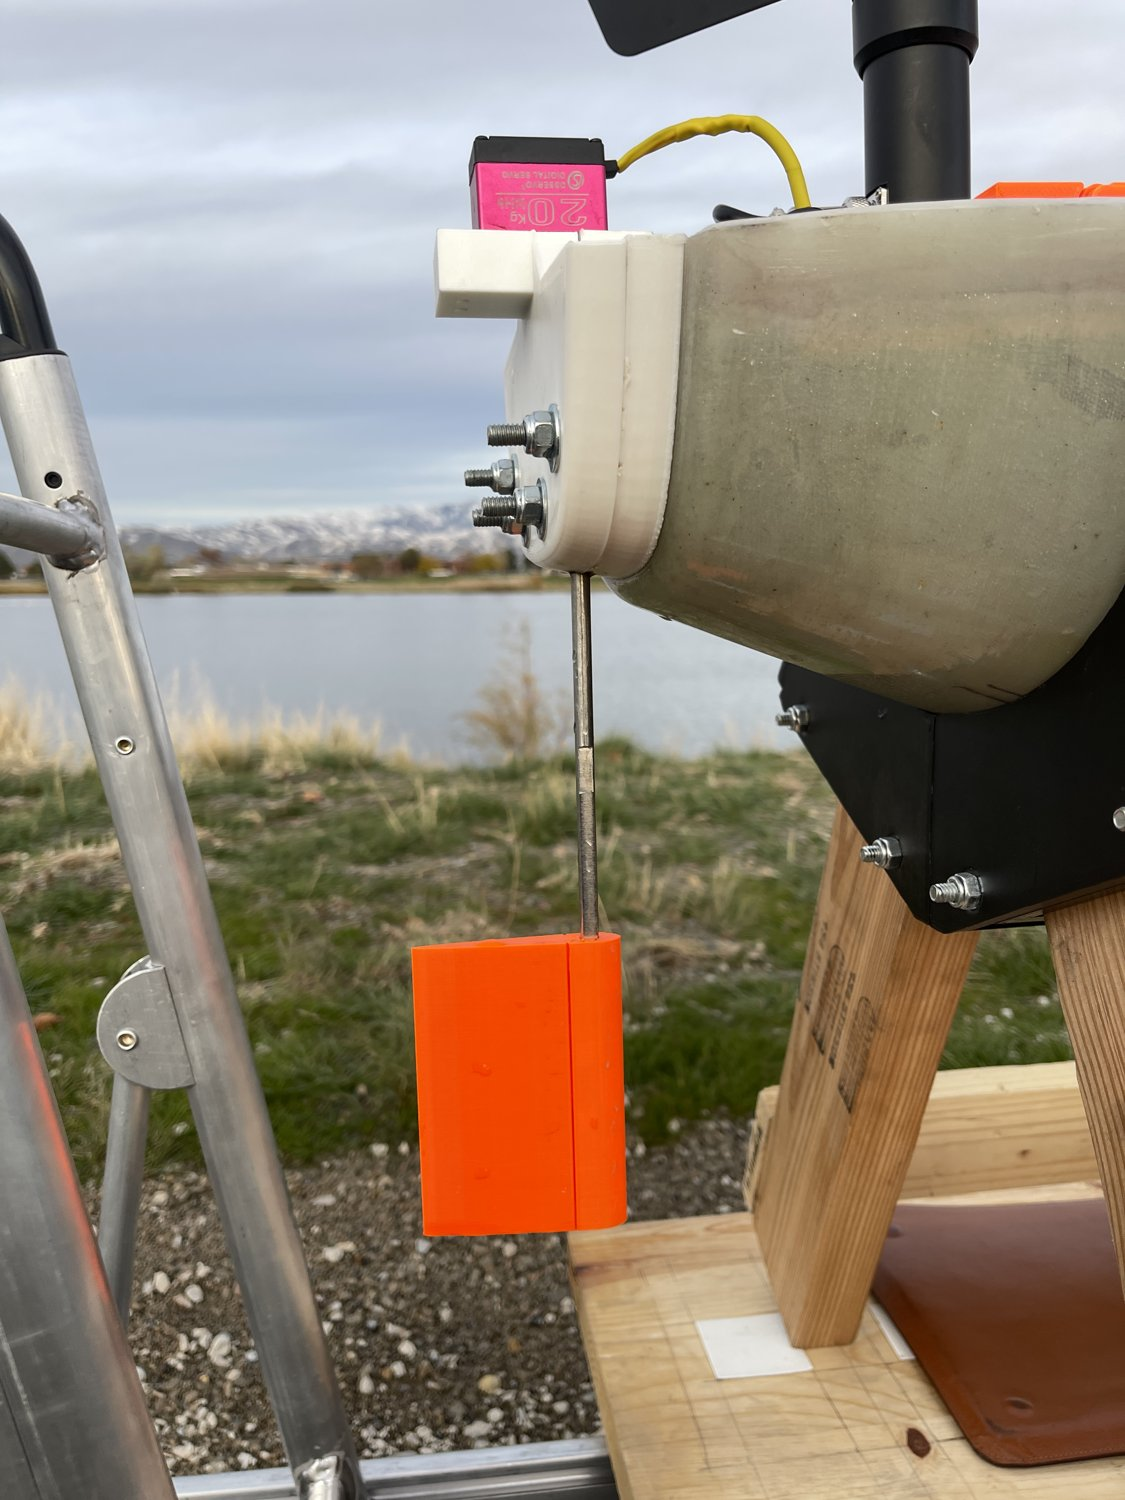
\includegraphics[height=3.2cm]{rudder_photo}}
\caption{Stern. (a) Exploded CAD of the rudder clamp, bearings, and shaft.
(b) Wind vane with its sealed aviation connector, cable glands, and the
rudder servo on its transom mount. (c) Printed rudder blade on the stainless
shaft below the transom.}
\label{fig:rudder}
\end{figure}

\subsection{Self-Trimming Wingsail}
The main wing and tail were carved from laminated XPS foam, which allowed a
wing more than \SI{1}{\meter} tall while keeping its mass low. The wing is
fixed to a \SI{3}{ft} 6061 aluminum mast tube that turns freely in a flanged ball-bearing unit at
deck level (Fig.~\ref{fig:sail}(d)). A printed collar with a radial arm
clamps the mast above the bearing and travels inside a printed guard ring
whose ends are hard stops, limiting the wing to $\pm\SI{90}{\degree}$ from
the centerline. A self-trimming wing never needs to point further aft than
abeam, and the stops protect the tail-servo cable routed through the mast. A \SI{10}{dBi} whip antenna for the
\SI{915}{\mega\hertz} radio is mounted at the masthead on a \SI{5}{ft} SubMiniature version A (SMA)
extension cable, which gives the radio the highest available mounting point
and a clear line of sight (Fig.~\ref{fig:sail}(e)).

Two carbon fiber booms carry the tail aft of the wing. In the proposal, a
servo inside the wing pushed and pulled the tail through a wire. As built,
the servo sits in a printed bracket on the lower boom and turns the tail's
lower pivot directly (Fig.~\ref{fig:sail}(b)), while the upper pivot runs in
a printed bearing housing on the upper boom (Fig.~\ref{fig:sail}(c)). Direct
drive removes the wire's backlash and stretch. The booms extend forward of the
mast to a printed counterweight (Fig.~\ref{fig:sail}(a)) sized so that
\begin{equation}
m_{cw}\, r_{cw} = \sum_i m_i\, r_i ,
\label{eq:balance}
\end{equation}
where the right-hand side sums the mass moments of the tail, servo, and aft
booms about the mast axis. Satisfying \eqref{eq:balance} places the combined center of gravity on the axis, so heel and pitch do not apply a rotating moment to the wing.

\begin{figure}[!t]
\centering
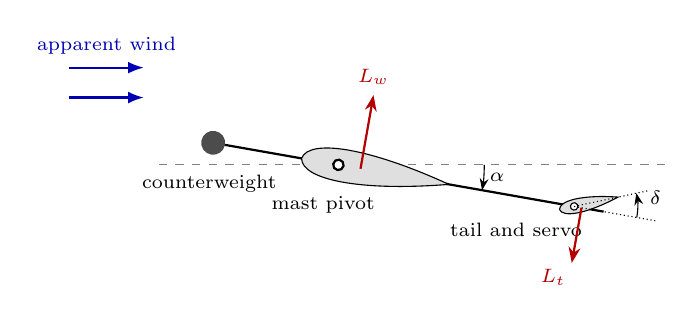
\begin{tikzpicture}[scale=0.95, every node/.style={font=\scriptsize}]
  % apparent wind (from left, +x)
  \foreach \y in {1.3,0.9}
    \draw[-{Latex[length=2mm]},thick,blue!70!black] (-3.6,\y) -- (-2.6,\y);
  \node[blue!70!black,anchor=south] at (-3.1,1.35) {apparent wind};
  \draw[dashed,gray] (-2.4,0) -- (4.4,0);
  \begin{scope}[rotate=-10]
    % boom
    \draw[thick] (-1.7,0) -- (3.6,0);
    % main wing (leading edge at -0.5, pivot at 0)
    \draw[fill=gray!25] (-0.5,0) .. controls (-0.45,0.28) and (0.35,0.3) .. (1.5,0)
                       .. controls (0.35,-0.3) and (-0.45,-0.28) .. (-0.5,0);
    % counterweight
    \fill[gray!60!black] (-1.7,0) circle (0.16);
    \node[anchor=north] at (-1.7,-0.3) {counterweight};
    % tail, deflected by delta about its pivot at 3.2
    \begin{scope}[shift={(3.2,0)}, rotate=22]
      \draw[fill=gray!25] (-0.2,0) .. controls (-0.18,0.12) and (0.15,0.13) .. (0.6,0)
                         .. controls (0.15,-0.13) and (-0.18,-0.12) .. (-0.2,0);
      \draw[densely dotted] (0,0) -- (1.0,0);
    \end{scope}
    \fill[white,draw=black] (3.2,0) circle (0.05);
    \draw[densely dotted] (3.2,0) -- (4.3,0);
    \draw[-{Stealth[length=1.5mm]}] (4.05,0) arc (0:22:0.85);
    \node at (4.25,0.3) {$\delta$};
    \node[anchor=north] at (2.45,-0.22) {tail and servo};
    % mast pivot
    \fill[white,draw=black,thick] (0,0) circle (0.07);
    \node[anchor=north] at (-0.15,-0.32) {mast pivot};
    % lift arrows
    \draw[-{Stealth[length=2mm]},red!70!black,thick] (0.3,0) -- (0.3,1.0) node[above] {$L_w$};
    \draw[-{Stealth[length=2mm]},red!70!black,thick] (3.3,0) -- (3.3,-0.75) node[below left=-2pt] {$L_t$};
  \end{scope}
  % angle of attack
  \draw[-{Stealth[length=1.5mm]}] (1.95,0) arc (0:-10:1.95);
  \node at (2.12,-0.17) {$\alpha$};
\end{tikzpicture}
\caption{Self-trimming wingsail seen from above. Deflecting the tail by
$\delta$ produces a tail lift $L_t$ whose moment about the mast pivot rotates
the wing until it balances the wing lift moment, settling at angle of attack
$\alpha$.}
\label{fig:stw}
\end{figure}

Fig.~\ref{fig:stw} shows why the wing trims itself. With dynamic pressure
$q$, wing and tail areas $S_w$ and $S_t$, signed moment arms $l_w$ and $l_t$
from the pivot to each surface's aerodynamic center, and lift coefficients
$C_{L,w}$ and $C_{L,t}$, the yawing moment about the mast is
\begin{equation}
M(\alpha,\delta) = q \left[ S_w l_w C_{L,w}(\alpha) + S_t l_t C_{L,t}(\alpha-\delta) \right].
\label{eq:moment}
\end{equation}
The wing rotates until $M = 0$ in \eqref{eq:moment}. Because $q$ multiplies both terms, the
equilibrium angle of attack depends on the tail deflection $\delta$ but not on
wind speed~\cite{elkaim2008}. Gusts therefore change the force on the sail but
not its trim, and shifts in wind direction are followed passively. Wind speed
does set how quickly the wing reaches equilibrium, which is the delayed
response noted in Table~\ref{tab:sailtypes} and the main challenge for the
sail controller in Section~\ref{sec:sw}.

\begin{figure*}[!t]
\centering
\subfloat[]{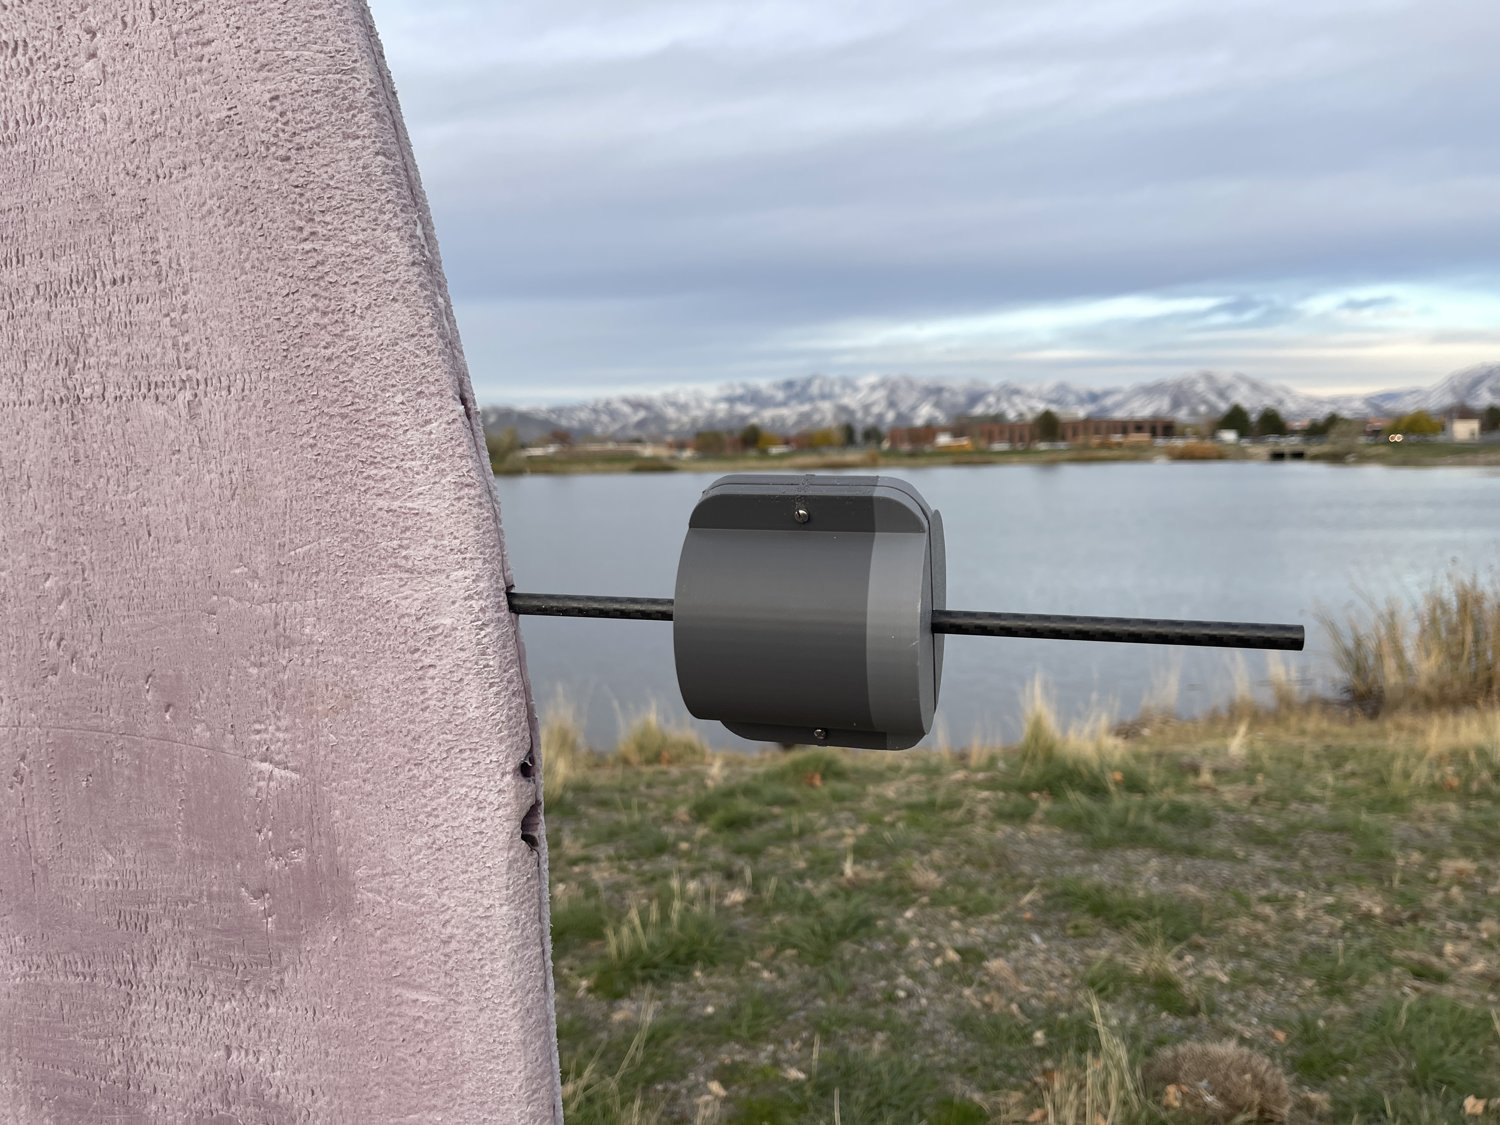
\includegraphics[height=2.55cm]{counterweight}}
\hfil
\subfloat[]{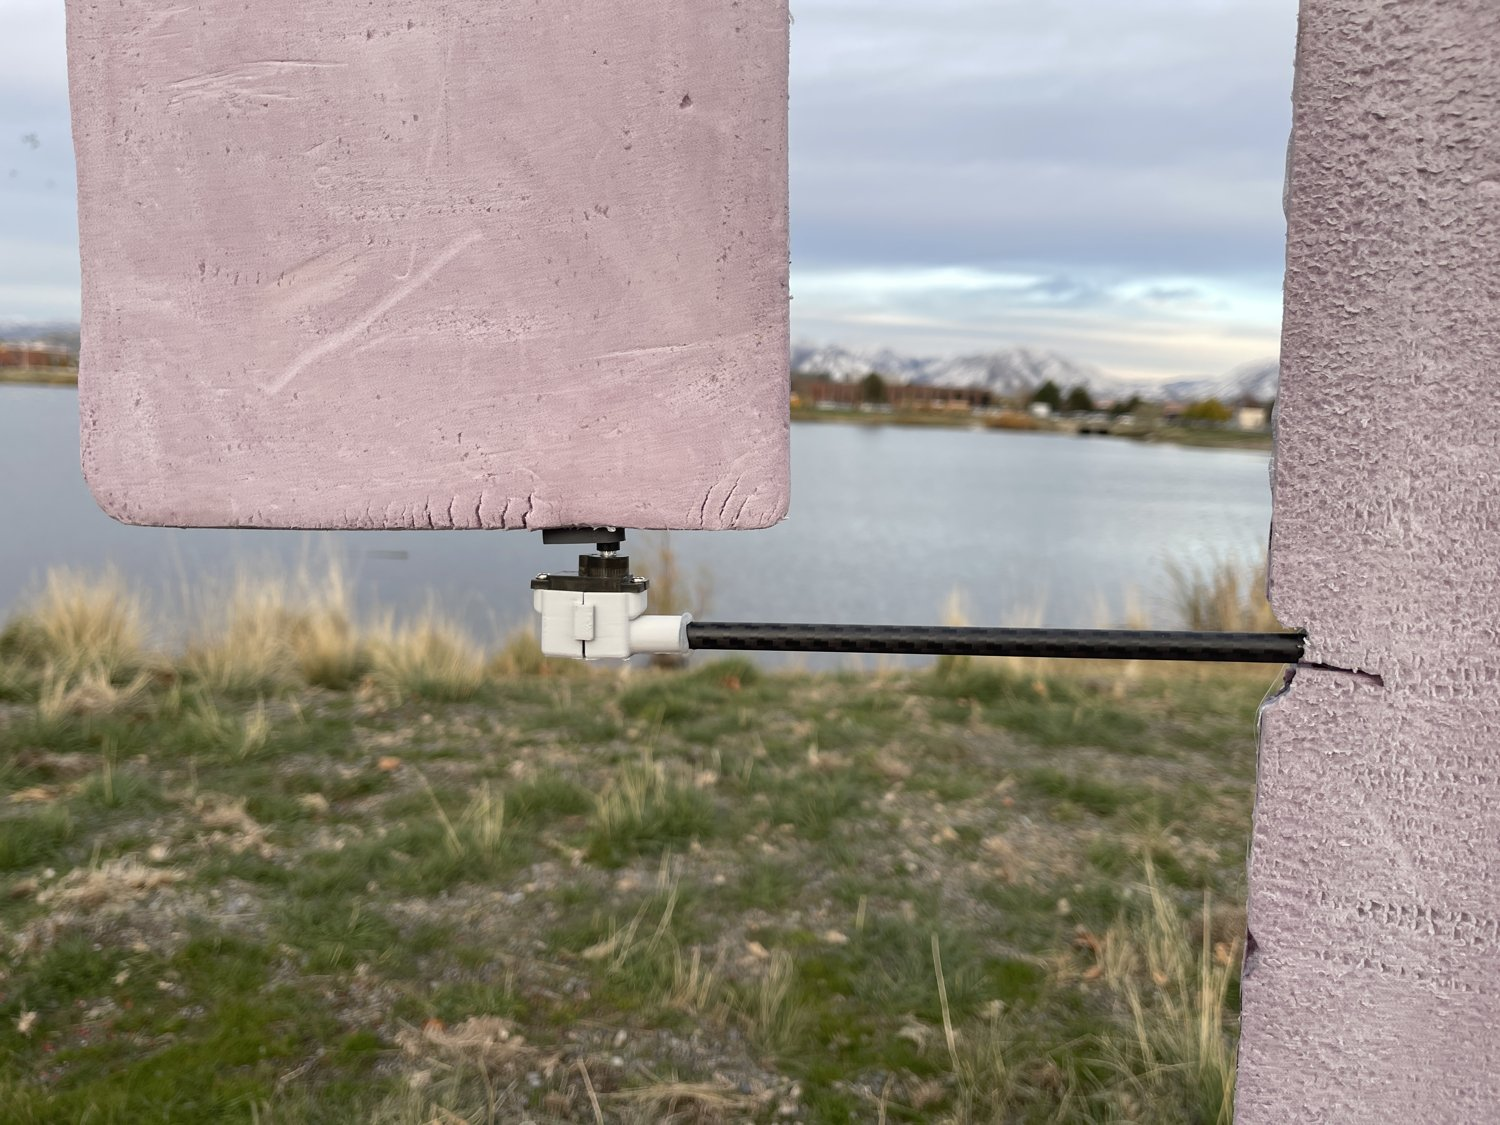
\includegraphics[height=2.55cm]{tail_servo}}
\hfil
\subfloat[]{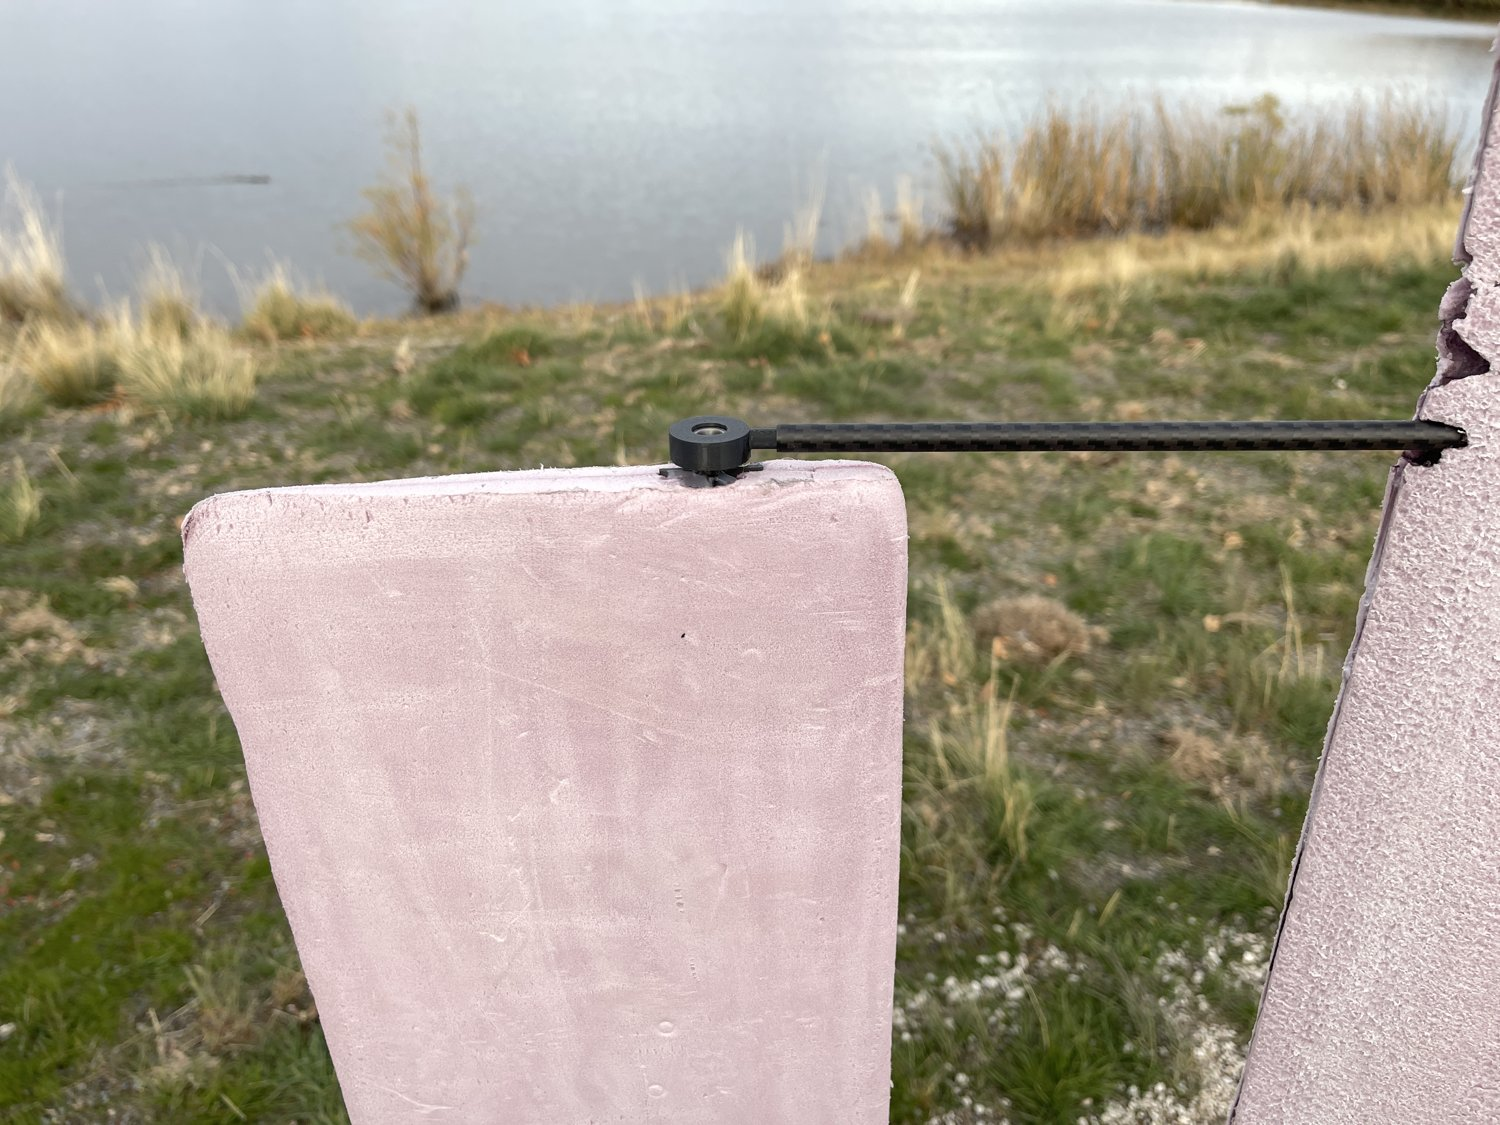
\includegraphics[height=2.55cm]{tail_pivot}}
\hfil
\subfloat[]{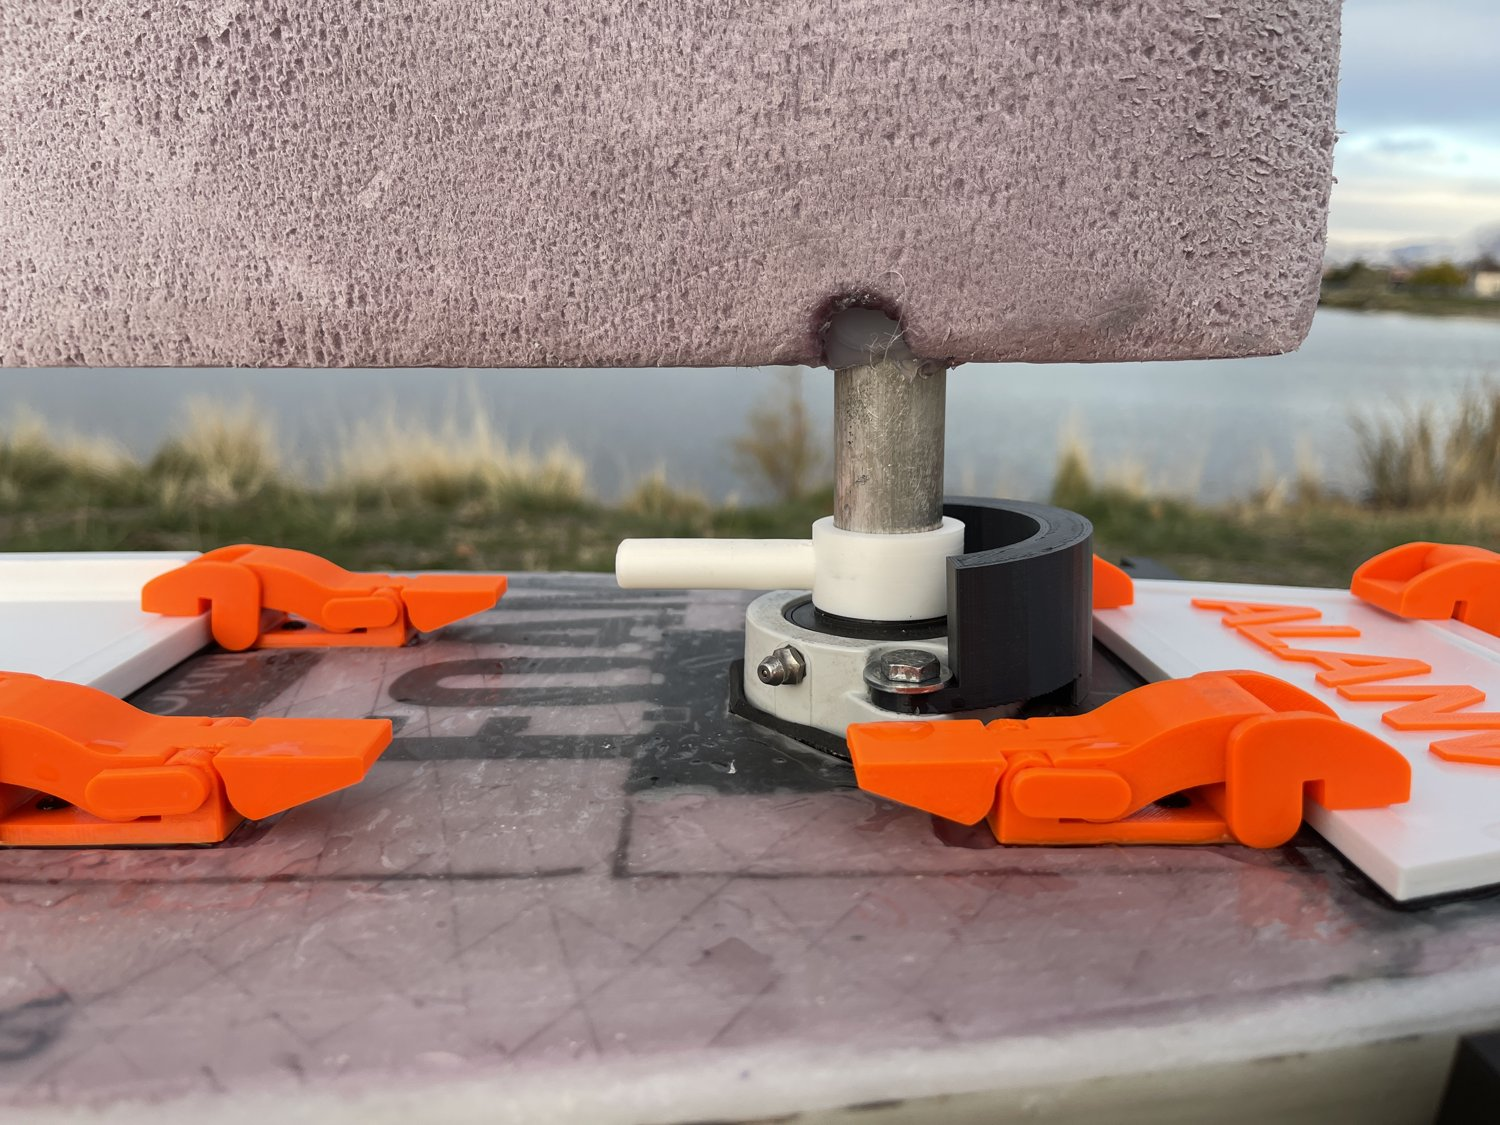
\includegraphics[height=2.55cm]{mast_base}}
\hfil
\subfloat[]{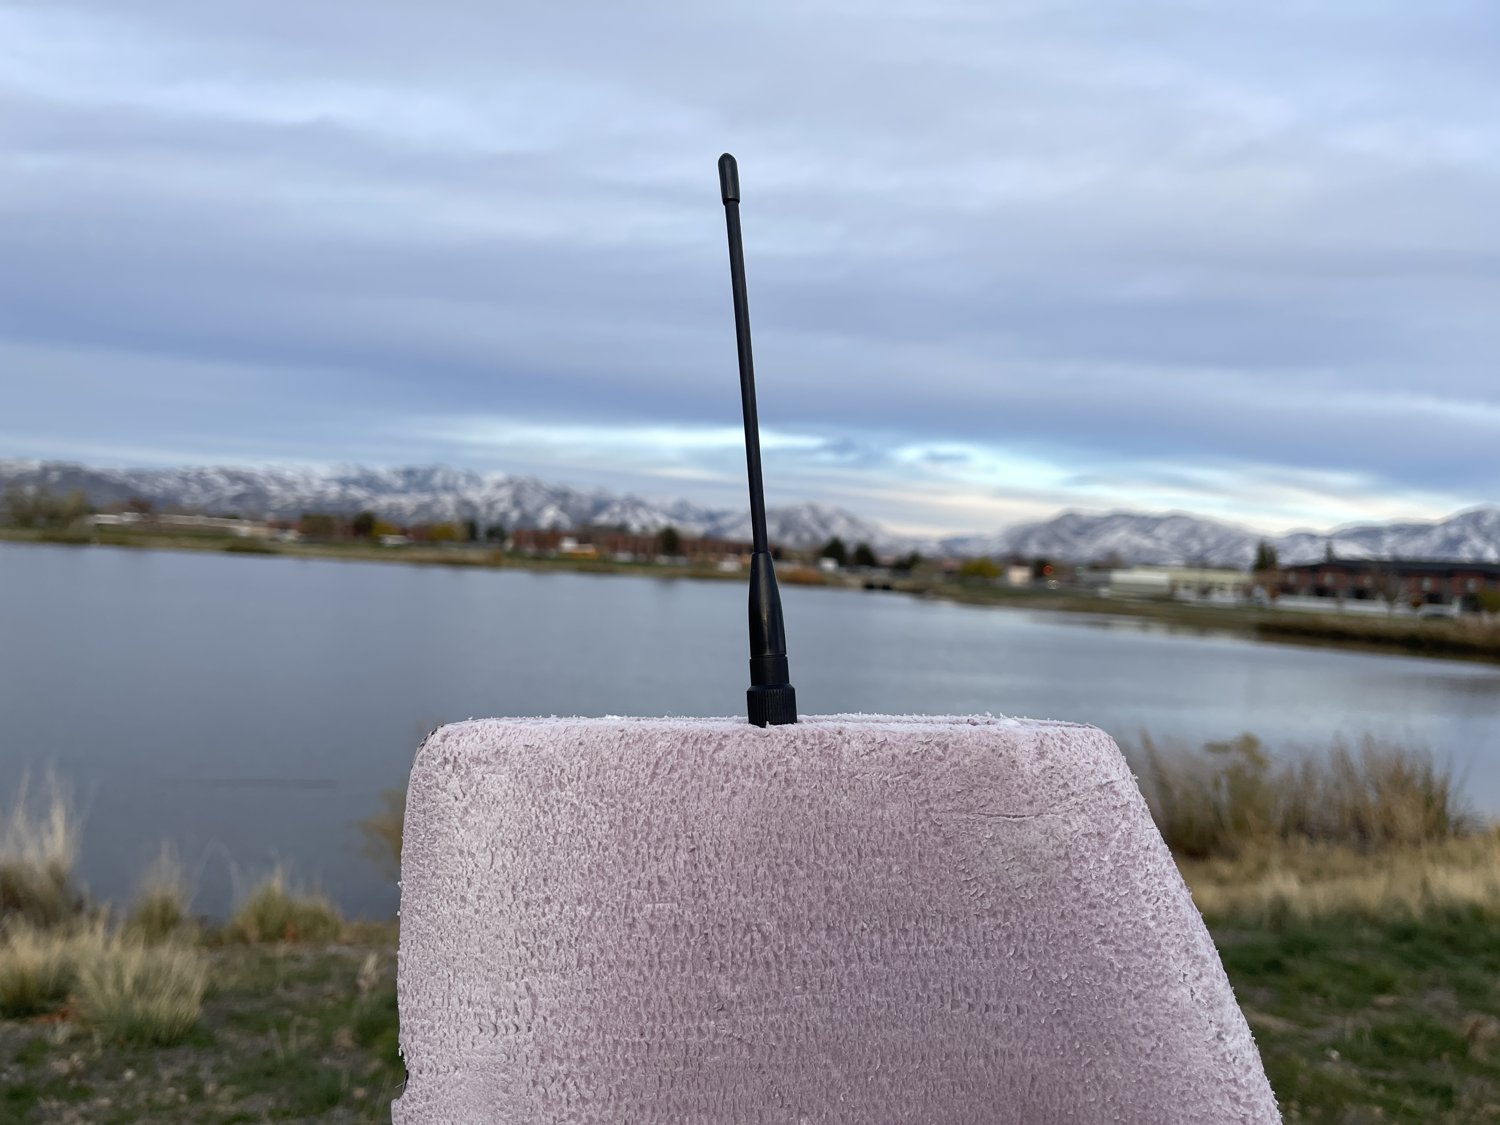
\includegraphics[height=2.55cm]{masthead_antenna}}
\caption{Wingsail hardware. (a) Printed counterweight on the forward boom
extension. (b) Tail servo in its printed bracket at the end of the lower
carbon boom, driving the tail's lower pivot. (c) Upper tail pivot bearing.
(d) Mast tube in the flanged ball-bearing unit, with the printed collar and
guard ring that form the $\pm\SI{90}{\degree}$ stops. (e) \SI{10}{dBi} LoRa
antenna at the masthead.}
\label{fig:sail}
\end{figure*}

The sail angle relative to the hull is measured below deck by an AS5600
12-bit magnetic rotary encoder at the mast step (Fig.~\ref{fig:deck}(b)). The
firmware treats one encoder revolution (4096 counts) as one revolution of the
wing, a resolution of \SI{0.088}{\degree}; the spur gearing between the mast
and the encoder is 1:1. Combined with the wind vane, this measurement closes the sail
control loop described in Section~\ref{sec:sw}.

\subsection{Integration and Balance}
\label{sec:integration}
The keel, rudder, and wing each join the hull at a single interface: the keel
bracket bolts through the reinforced keel boss, the rudder shaft turns in its
two-part bearing clamp at the transom, and the mast seats in the mast step
(Fig.~\ref{fig:cad}(b)). Each can be removed for repair without disturbing
the others. The two ballast canisters are the main trim adjustment; loading
them unevenly moves the center of mass fore and aft without changing the
hull.

The simulator's hydrostatic model (Section~\ref{sec:test}) floats a voxel
model of the CAD at its \SI{4.9}{\kilo\gram} mass. It predicts
\SI{141}{\milli\meter} of freeboard, \SI{1}{\degree} of bow-up trim, and a
total draft of \SI{307}{\milli\meter}. The righting moment stays positive to
\SI{175}{\degree} of heel, peaking at about \SI{12}{\newton\meter} near
\SI{80}{\degree}, so the ballasted keel alone makes the boat effectively
self-righting. The field test agrees: the median heel was \SI{13}{\degree},
and the boat recovered from a peak of \SI{60}{\degree} without capsizing.

At the self-trimming equilibrium the aerodynamic moment about the mast is
zero, so the sail force acts through the mast step,
\SI{107}{\milli\meter} forward of the hull's midpoint. The geometric CLR of
the hull and keel lies \SI{14}{\milli\meter} aft of the midpoint, so the COE
leads it by about \SI{120}{\milli\meter}. Because the keel's lift acts near
its quarter chord and heel adds weather helm, the effective balance is closer
than this estimate. The helm has not been measured directly; in the field
test, the heading PID held 2 to \SI{6}{\degree} of rudder to the same side on
both tacks, which suggests a small rudder-centering offset.

\section{Electrical Design}
\label{sec:elec}

\subsection{Power}
A four-cell (4S) LiPo battery, \SI{14.8}{\volt} nominal,
supplies the boat through XT60 connectors and a power distribution board that
provides regulated rails for the servos and logic. The regulator outputs a 12V rail that powers out wind vane, and it outputs a 5V rail that powers the rudder and sail-tail servos as well as the STM32 board. Our battery capacity is rated for 1300 mAh.

The pack is monitored without a dedicated battery-monitor chip. Each
cumulative cell tap (cell 1, cells 1--2, cells 1--3, and the full pack) feeds
an analog-to-digital converter (ADC) channel through a divider with
$R_{\mathrm{top}} = \SI{82}{\kilo\ohm}$ and
$R_{\mathrm{bot}} = \SI{18}{\kilo\ohm}$, so the tap voltage is
\begin{equation}
V_{\mathrm{tap}} = V_{\mathrm{pin}}\,\frac{R_{\mathrm{top}} + R_{\mathrm{bot}}}{R_{\mathrm{bot}}}
               = 5.56\,V_{\mathrm{pin}} .
\label{eq:divider}
\end{equation}
By~\eqref{eq:divider}, a fully charged pack (\SI{16.8}{\volt}) appears as \SI{3.02}{\volt},
just inside the \SI{3.3}{\volt} ADC reference. A \SI{100}{\nano\farad}
capacitor across each divider forms a low-pass filter with a time constant of
about \SI{1.5}{\milli\second}. The firmware waits \SI{10}{\milli\second}
(about seven time constants) before converting and averages eight conversions per
channel in integer arithmetic. It samples at \SI{2}{\hertz} and averages the
last 20 readings, a ten-second window, before recovering each cell voltage by
subtracting adjacent taps. Pin PA1 was avoided because the Nucleo board ties it to the
Ethernet physical-layer clock, which injects noise.

\subsection{Sensors and Actuators}
Table~\ref{tab:elec} lists the components, the peripheral each uses, and its
sample rate. The BNO055 combines a three-axis accelerometer, gyroscope, and
magnetometer with onboard fusion~\cite{bno055}, so it supplies both the
IMU and magnetometer called for in the proposal;
it runs in its nine-degree-of-freedom (NDOF) fusion mode with stored
calibration offsets. The AS5600~\cite{as5600} measures sail angle. The BNO055 and AS5600 connect over separate inter-integrated circuit (I\textsuperscript{2}C) buses. The DFRobot wind
vane has an adapter that converts to a universal asynchronous receiver-transmitter (UART) signal for
the microcontroller. It is polled with a Modbus RTU ``read holding register''
request~\cite{modbus} protected by a 16-bit cyclic redundancy check (CRC) and reports apparent wind
direction in tenths of a degree. The u-blox NEO-6 GPS receiver streams National Marine Electronics Association (NMEA) 0183
sentences~\cite{nmea0183}; the firmware receives them by direct memory access
(DMA) with idle-line detection and parses the GGA sentence for position, fix
quality, and satellite count, and the RMC sentence for speed and course over
ground, which the tack planner uses. Position is marked valid only while the
most recent GGA sentence reported a fix.

Both servos are driven by pulse-width modulation (PWM) from timer TIM1 at \SI{50}{\hertz}, with pulse widths
from \SI{500}{\micro\second} to \SI{2500}{\micro\second} mapped linearly to
$\pm\SI{90}{\degree}$.

\begin{table}[!t]
\caption{Electronic Components and Interfaces}
\label{tab:elec}
\centering
\begin{tabular}{@{}p{0.2\columnwidth}p{0.36\columnwidth}p{0.32\columnwidth}@{}}
\toprule
Function & Component & Interface, rate \\
\midrule
Controller   & NUCLEO-H755ZI-Q (STM32H755) & -- \\
Orientation  & Bosch BNO055, NDOF mode & I\textsuperscript{2}C2, \SI{50}{\hertz} \\
Sail angle   & ams AS5600 12-bit encoder & I\textsuperscript{2}C1, \SI{10}{\hertz} \\
Wind         & DFRobot RS-485 wind vane, Modbus RTU & UART4 via RS-485 adapter, \SI{5}{\hertz} \\
Position     & u-blox NEO-6 GPS, NMEA GGA & UART7 + DMA, \SI{1}{\hertz} \\
Battery      & Four divider taps & ADC1, \SI{2}{\hertz} \\
Telemetry    & RFM95W (SX1276) LoRa & SPI1 on CM4, \SI{1}{\hertz} \\
Rudder       & DS3218MG 20 kg-cm servo & TIM1 PWM, \SI{50}{\hertz} \\
Tail         & MG90S 9G Servo & TIM1 PWM, \SI{50}{\hertz} \\
Debug        & ST-LINK virtual COM port & USART3, 115200 Bd \\
\bottomrule
\end{tabular}
\end{table}

\subsection{Communication Link}
The boat communicates with an elevated ground station over line of sight. The
team chose LoRa (long range) modulation~\cite{augustin2016} over Wi-Fi or
Bluetooth because the traffic is small and infrequent and because low power
consumption is a design priority. LoRa operates in the unlicensed industrial,
scientific, and medical (ISM) bands, at \SI{915}{\mega\hertz} in North
America. Sub-gigahertz signals reach farther than \SI{2.4}{\giga\hertz}
signals because they diffract more readily around obstacles and because
free-space path loss (FSPL) grows with frequency:
\begin{equation}
\mathrm{FSPL} = 20\log_{10} d + 20\log_{10} f + 20\log_{10}\!\left(\frac{4\pi}{c}\right),
\label{eq:fspl}
\end{equation}
with distance $d$ in meters, frequency $f$ in hertz, and $c$ the speed of
light. At \SI{1}{\kilo\meter}, \eqref{eq:fspl} gives \SI{91.7}{dB} at
\SI{915}{\mega\hertz} and \SI{100.0}{dB} at \SI{2.4}{\giga\hertz}, an
\SI{8.4}{dB} advantage that corresponds to about 2.6 times the range for the
same link budget.

The RFM95W module (Semtech SX1276 transceiver~\cite{sx1276}) is configured for
spreading factor (SF) 8, \SI{125}{\kilo\hertz} bandwidth (BW), coding rate (CR) 4/5,
explicit header, hardware CRC, and \SI{17}{dBm} output on the PA\_BOOST pin. The CM4 talks to the module over the serial peripheral interface (SPI).
The time on air of one packet follows from the symbol time
$T_s = 2^{\mathrm{SF}}/\mathrm{BW}$ and the payload symbol
count~\cite{sx1276}
\begin{multline}
n_{\mathrm{pl}} = 8 + \max\Bigl(\Bigl\lceil \tfrac{8L - 4\,\mathrm{SF} + 28 + 16\,\mathrm{CRC} - 20\,\mathrm{IH}}{4(\mathrm{SF} - 2\,\mathrm{DE})} \Bigr\rceil (\mathrm{CR}+4),\, 0\Bigr),\\
T_{\mathrm{air}} = (n_{\mathrm{pre}} + 4.25 + n_{\mathrm{pl}})\,T_s ,
\label{eq:airtime}
\end{multline}
where $L$ is the payload length in bytes, CRC $=1$, implicit header IH $=0$,
low-data-rate optimization DE $=0$, CR $=1$, and $n_{\mathrm{pre}} = 8$. Applying~\eqref{eq:airtime} to
the 78-byte telemetry frame of Section~\ref{sec:sw} gives $T_s =
\SI{2.048}{\milli\second}$, $n_{\mathrm{pl}} = 108$, and $T_{\mathrm{air}}
\approx \SI{246}{\milli\second}$. Sent once per second, telemetry occupies
about a quarter of the channel; the radio spends the remaining time listening
for commands.

\subsection{Packaging}
The electronics are mounted in a printed enclosure that drops into the aft
hatch (Fig.~\ref{fig:electronics}). The microcontroller board is mounted along
one wall, with the radio, GPS receiver, and orientation sensor on printed
standoffs. The BNO055 is mounted flat and fixed to the hull so that its axes
stay aligned with the boat's. External cables enter through compression
glands, and the antenna feed passes through a sealed SMA bulkhead connector to
the masthead antenna. Interconnections are made on a solderless
breadboard. A KiCad schematic for a custom carrier board around the STM32H755
was started, but the board is no longer planned, so the breadboard remains in
the vessel as built. Its solderless contacts are vulnerable to vibration and
corrosion on the water.

\begin{figure}[!t]
\centering
\subfloat[]{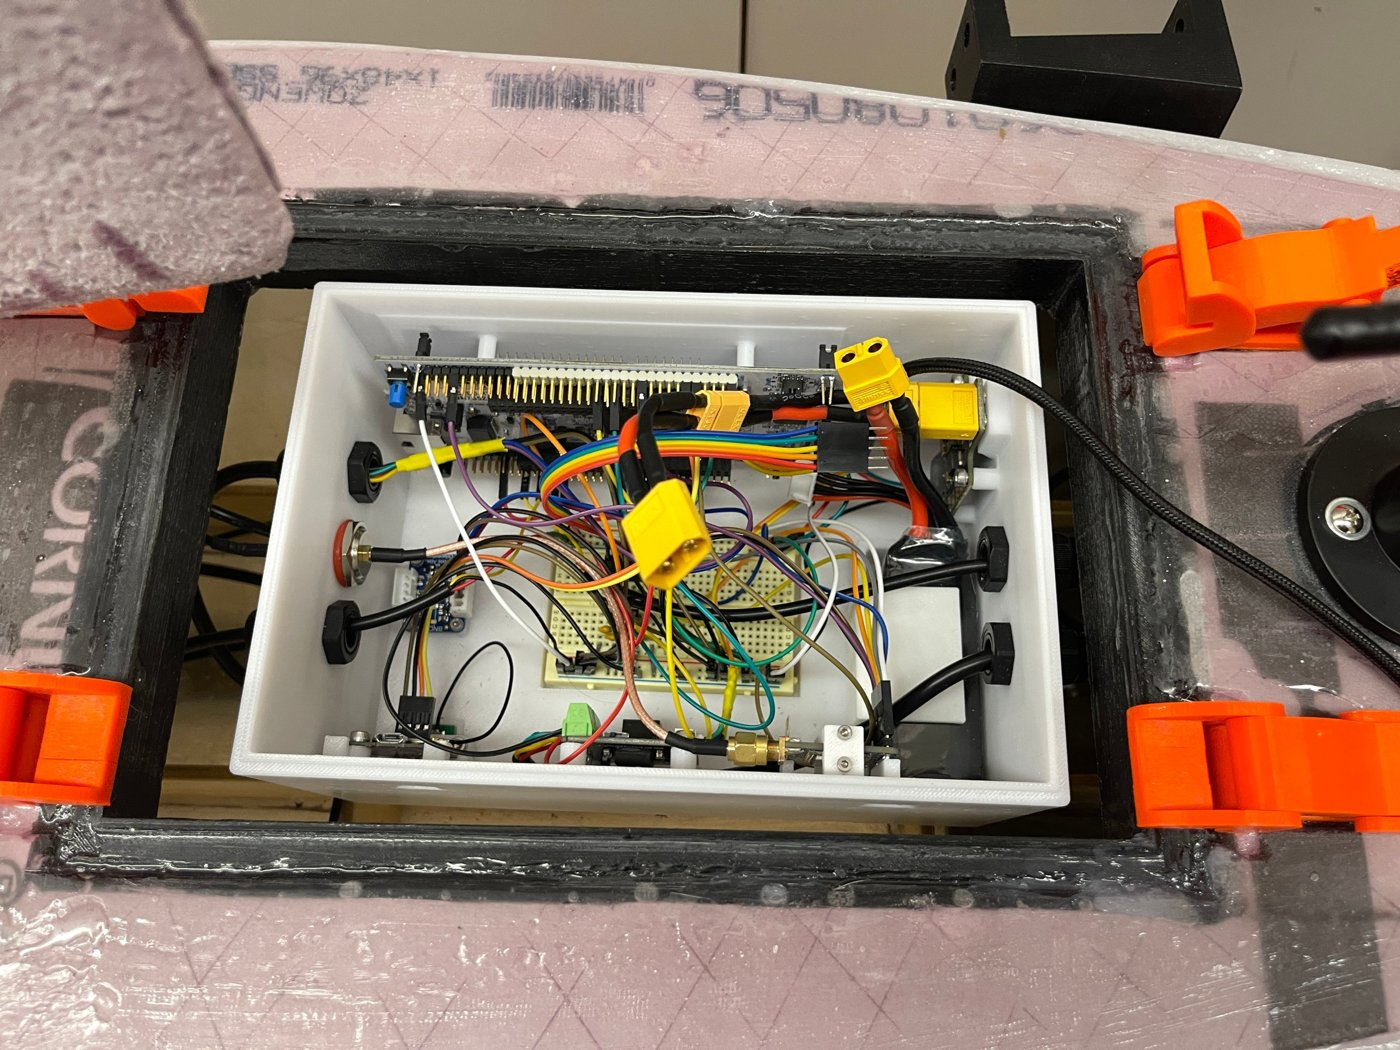
\includegraphics[width=0.56\columnwidth]{electronics_box}}
\hfil
\subfloat[]{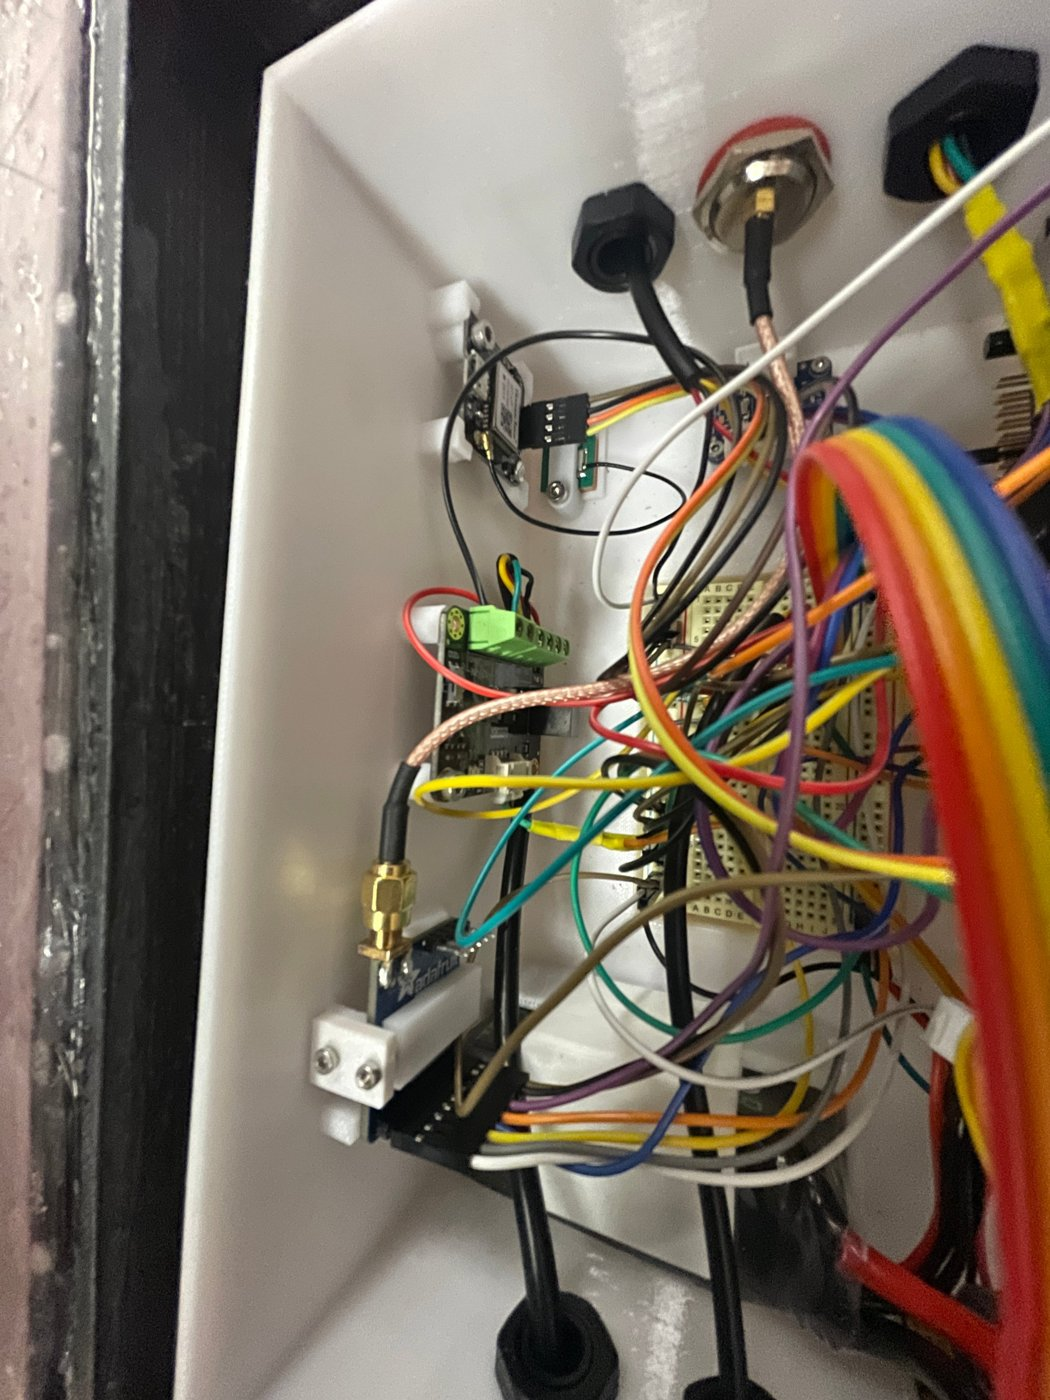
\includegraphics[width=0.33\columnwidth]{electronics_side}}
\caption{Electronics enclosure in the aft hatch. (a) Overview: NUCLEO-H755ZI-Q
board, power distribution board and XT60 connectors, breadboard, BNO055, and
cable glands. (b) Side wall: NEO-6 GPS module, RS-485 adapter for the wind vane, and LoRa
radio with its SMA feed to the bulkhead connector.}
\label{fig:electronics}
\end{figure}

\section{Software Architecture}
\label{sec:sw}

This section describes the firmware on the \texttt{ltp} branch (commit
\texttt{ca2e48e}), the most recent version. It merges the \texttt{master}
branch with the tack planner and the sensor and stack updates from
\texttt{sensor-upgrade-2}. The firmware is written in C on the STM32 hardware
abstraction layer (HAL),
about 8000 lines of application code across the two cores and a shared
library. It is built with CMake. A single shared configuration header enables
or disables each module at compile time, so any subsystem can be built and
tested alone. The same header selects built-in test modes.

\subsection{Dual-Core Partitioning}
The STM32H755 has a Cortex-M7 and a Cortex-M4 that share memory but run
separate firmware images~\cite{rm0399}. ALAN divides the work by timing
requirement. The CM7 runs the FreeRTOS real-time operating system
(RTOS)~\cite{barry2016} and owns every sensor, both planners and control
loops, both actuators, and the mode logic. The CM4 runs without an operating
system and owns only the radio. Its main loop sleeps on a wait-for-interrupt
instruction and wakes for two events: the radio's DIO0 line, which signals a
finished transmission or a received packet, and timer TIM6, which fires once
per second to start a telemetry transmission. Because radio transfers and
timeouts happen on the other core, they cannot delay a control loop.

\subsection{Inter-Core Communication}
\label{sec:ipc}
The cores exchange data only through a \SI{64}{\kilo\byte} block of SRAM4 at
address \texttt{0x38000000}, which both linker scripts place at the same
address (Fig.~\ref{fig:ipc}). At boot the CM7 configures its memory protection
unit (MPU) to make the region non-cacheable, clears it, and writes a layout
version followed by a magic word (``ALAN'' in ASCII). The CM4 waits for the
magic word and refuses to attach if the version, which combines a revision
number with the structure size, does not match its own. This catches the
common mistake of flashing the cores with different layouts. The block holds
two channels:
\begin{itemize}
\item \emph{Telemetry} (CM7 to CM4): a single latest-value copy of the
telemetry record, guarded by hardware semaphore (HSEM) 1. Only the newest
record matters, so a core that finds the semaphore taken skips that cycle
instead of waiting.
\item \emph{Commands} (CM4 to CM7): a lock-free single-producer,
single-consumer ring of 64 slots of 18 bytes (type, sequence number, and a
16-byte payload). The CM4 writes only the head index and the CM7 only the
tail, and memory barriers order each slot write before its index update.
After each push the CM4 takes and releases HSEM 2, which raises an interrupt
on the CM7 that wakes the command task.
\end{itemize}

\begin{figure}[!t]
\centering
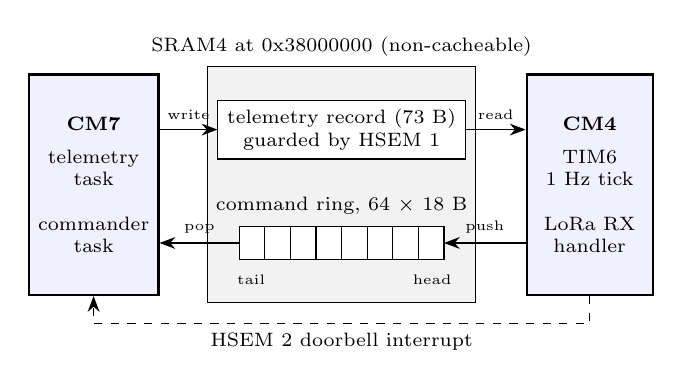
\begin{tikzpicture}[font=\scriptsize, >={Stealth[length=2mm]}]
\node[draw, thick, fill=blue!6, minimum width=16mm, minimum height=28mm, align=center] (m7) at (0,0) {\textbf{CM7}\\[4pt]telemetry\\task\\[8pt]commander\\task};
\node[draw, thick, fill=blue!6, minimum width=16mm, minimum height=28mm, align=center] (m4) at (6.3,0) {\textbf{CM4}\\[4pt]TIM6\\1 Hz tick\\[8pt]LoRa RX\\handler};
\node[draw, fill=gray!10, minimum width=34mm, minimum height=30mm] (s) at (3.15,0) {};
\node[anchor=south, align=center] at (s.north) {SRAM4 at 0x38000000 (non-cacheable)};
\node[draw, fill=white, minimum width=29mm, align=center] (tr) at (3.15,0.7) {telemetry record (73 B)\\guarded by HSEM 1};
\foreach \i in {0,...,7} \draw[fill=white] (1.85+\i*0.325,-0.95) rectangle ++(0.325,0.42);
\node at (3.15,-0.27) {command ring, 64 $\times$ 18 B};
\node[font=\tiny] at (2.0,-1.2) {tail};
\node[font=\tiny] at (4.3,-1.2) {head};
\draw[->] (m7.east |- tr) -- node[above,font=\tiny]{write} (tr.west);
\draw[->] (tr.east) -- node[above,font=\tiny]{read} (m4.west |- tr);
\draw[->] (m4.west |- 0,-0.74) -- node[above,font=\tiny]{push} (4.45,-0.74);
\draw[->] (1.85,-0.74) -- node[above,font=\tiny]{pop} (m7.east |- 0,-0.74);
\draw[->, dashed] (m4.south) -- ++(0,-0.35) -| node[pos=0.25,below]{HSEM 2 doorbell interrupt} (m7.south);
\end{tikzpicture}
\caption{Inter-core communication. Telemetry is a single latest-value record
under a hardware semaphore; commands use a lock-free ring, and a second
semaphore acts as a doorbell that wakes the CM7.}
\label{fig:ipc}
\end{figure}

\subsection{Task Structure and Data Flow}
Table~\ref{tab:tasks} lists the CM7 tasks. Every periodic task waits on
\texttt{vTaskDelayUntil}, so its period is fixed and each PID uses a constant
sample time. Each sensor task publishes its latest result to a single-slot
FreeRTOS queue that is overwritten on every update. Every result carries a
timestamp, a validity code (for example valid, calibrating, window filling,
or untrusted), and a sequence number, so consumers can reject stale or bad
data instead of acting on it. Priorities follow consequence. The commander
runs highest so a mode change takes effect at once. The arbiters and the
telemetry task run above the sensor drivers, whose I\textsuperscript{2}C and
UART reads busy-wait, so servo outputs and the SRAM4 publish are never
starved. The planners run lowest.

\begin{table}[!t]
\caption{CM7 FreeRTOS Tasks}
\label{tab:tasks}
\centering
\begin{tabular}{@{}llr@{}}
\toprule
Task & Priority & Rate (Hz) \\
\midrule
Commander (modes, commands) & High         & event, 10 \\
Telemetry packing           & Above normal & 1 \\
Rudder arbiter              & Above normal & 20 \\
Tail arbiter                & Above normal & 20 \\
Heading PID                 & Normal       & 10 \\
Sail PID                    & Normal       & 10 \\
IMU (BNO055)                & Normal       & 50 \\
Sail encoder (AS5600)       & Normal       & 10 \\
Orientation fusion          & Normal       & on IMU data \\
Wind vane                   & Normal       & 5 \\
GPS                         & Low          & 1 \\
Battery                     & Low          & 2 \\
Live sail planner (LSP)     & Low          & 2 \\
Live tack planner (LTP)     & Normal       & 2 \\
Serial console (debug)      & Low          & on demand \\
\bottomrule
\end{tabular}
\end{table}

Angles need care when averaged. The encoder jumps from 4095 to 0 counts once
per turn, and the wind vane does the same at \SI{180}{\degree}, so a plain
average of readings that straddle the seam points in the opposite direction.
Both drivers instead track a continuous, \emph{unwrapped} count
\begin{equation}
u_k = u_{k-1} + \mathrm{wrap}_{\pm N/2}\!\left(r_k - r_{k-1}\right),
\label{eq:unwrap}
\end{equation}
where $r_k$ is the raw reading and $N$ the counts per turn, and the wind driver averages $u$ from~\eqref{eq:unwrap} over 20 samples with a
running sum. The encoder driver originally did the same over ten samples. On
the final firmware it reads at \SI{10}{\hertz} without averaging, because its
readings proved stable and the $\pm\SI{90}{\degree}$ stops keep the wing from
reaching the seam. The
navigation code uses the circular mean
$\bar{\theta} = \operatorname{atan2}(\sum\sin\theta_i, \sum\cos\theta_i)$ for
the same reason.

The fusion task wakes on each new IMU sample. It averages the last ten BNO055
quaternions, normalizes the result, and converts it to Euler angles. Heading is
corrected from magnetic to true north with the local declination
(\SI{11}{\degree} in Salt Lake City) and for the sensor's mounting offset. The
task also estimates surge speed from successive GPS fixes.

\subsection{Sail and Heading Control}
Fig.~\ref{fig:control} shows the two control chains. Each consists of a
target source, a PID controller, an arbiter, and a servo. The PID
implementation~\cite{astrom1995} computes
\begin{align}
u_k &= \mathrm{sat}\!\left(K_p e_k + I_k - K_d\,\frac{y_k - y_{k-1}}{T}\right), \label{eq:pid}\\
I_k &= I_{k-1} + K_i T e_k , \label{eq:integral}
\end{align}
where $e_k$ is the error wrapped to $\pm\SI{180}{\degree}$, $y_k$ the measured
angle, and $T$ the sample period. In~\eqref{eq:pid}, the derivative acts on the measurement
rather than the error, so a new target does not cause a derivative kick. The
integral update~\eqref{eq:integral} is skipped whenever the output is
saturated in the direction of the error, which prevents windup, and the controller resets after a new target or a
gap in data.

\begin{figure*}[!t]
\centering
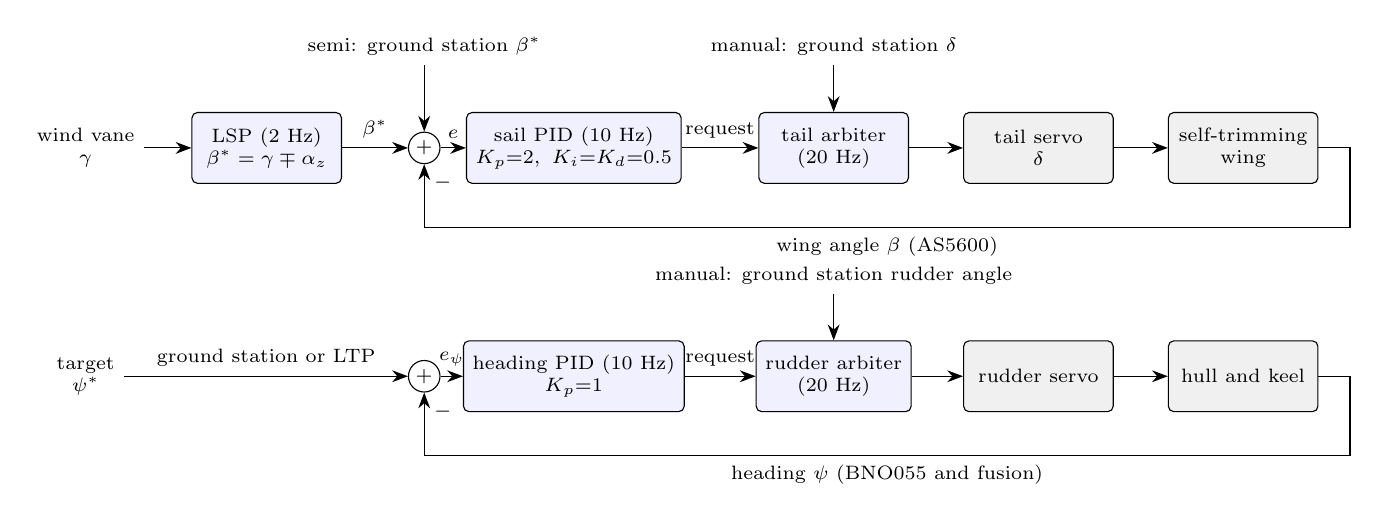
\begin{tikzpicture}[
  font=\scriptsize, >={Stealth[length=2mm]},
  b/.style={draw, rounded corners=2pt, fill=blue!6, align=center, minimum height=9mm, minimum width=19mm},
  p/.style={draw, rounded corners=2pt, fill=gray!12, align=center, minimum height=9mm, minimum width=19mm},
  sum/.style={draw, circle, inner sep=1.2pt}
]
% sail chain
\node[align=center] (vane) at (0,0) {wind vane\\$\gamma$};
\node[b] (lsp) at (2.3,0) {LSP (2 Hz)\\$\beta^{*} = \gamma \mp \alpha_z$};
\node[sum] (s1) at (4.3,0) {$+$};
\node[b] (pids) at (6.2,0) {sail PID (10 Hz)\\$K_p{=}2,\ K_i{=}K_d{=}0.5$};
\node[b] (arbt) at (9.5,0) {tail arbiter\\(20 Hz)};
\node[p] (tsv) at (12.1,0) {tail servo\\$\delta$};
\node[p] (wing) at (14.7,0) {self-trimming\\wing};
\draw[->] (vane) -- (lsp);
\draw[->] (lsp) -- node[above]{$\beta^{*}$} (s1);
\draw[->] (s1) -- node[above]{$e$} (pids);
\draw[->] (pids) -- node[above]{request} (arbt);
\draw[->] (arbt) -- (tsv);
\draw[->] (tsv) -- (wing);
\draw[->] (wing.east) -- ++(0.4,0) |- node[pos=0.75,below]{wing angle $\beta$ (AS5600)} ([yshift=-8mm]s1.south) -- node[pos=0.7,right]{$-$} (s1.south);
\draw[->] (4.3,1.05) node[above]{semi: ground station $\beta^{*}$} -- (s1.north);
\draw[->] (9.5,1.05) node[above]{manual: ground station $\delta$} -- (arbt.north);
% heading chain
\begin{scope}[yshift=-2.9cm]
\node[align=center] (src) at (0,0) {target\\$\psi^{*}$};
\node[sum] (s2) at (4.3,0) {$+$};
\node[b] (pidh) at (6.2,0) {heading PID (10 Hz)\\$K_p{=}1$};
\node[b] (arbr) at (9.5,0) {rudder arbiter\\(20 Hz)};
\node[p] (rsv) at (12.1,0) {rudder servo};
\node[p] (hull) at (14.7,0) {hull and keel};
\draw[->] (src) -- node[above]{ground station or LTP} (s2);
\draw[->] (s2) -- node[above]{$e_\psi$} (pidh);
\draw[->] (pidh) -- node[above]{request} (arbr);
\draw[->] (arbr) -- (rsv);
\draw[->] (rsv) -- (hull);
\draw[->] (hull.east) -- ++(0.4,0) |- node[pos=0.75,below]{heading $\psi$ (BNO055 and fusion)} ([yshift=-8mm]s2.south) -- node[pos=0.7,right]{$-$} (s2.south);
\draw[->] (9.5,1.05) node[above]{manual: ground station rudder angle} -- (arbr.north);
\end{scope}
\end{tikzpicture}
\caption{Sail (top) and heading (bottom) control chains. In AUTO the planners
set the targets; in SEMI the ground station sets the PID target; in MANUAL the
arbiter passes the ground-station servo angle straight through.}
\label{fig:control}
\end{figure*}

\paragraph*{Live sail planning}
The wind vane gives the apparent wind angle $\gamma$ relative to the bow
(positive from starboard), and the encoder gives the wing angle $\beta$ on the
same scale. The angle of attack is therefore $\alpha = \gamma - \beta$. The
live sail planner (LSP) chooses a wing-angle target that points the wing into
the apparent wind and then rotates it toward the bow by an angle of attack
$\alpha_z$ that depends on the point of sail:
\begin{equation}
\beta^{*} = \mathrm{wrap}_{\pm 180}\bigl(\gamma - \operatorname{sgn}(\gamma)\,\alpha_z(|\gamma|)\bigr),
\label{eq:lsp}
\end{equation}
with $\alpha_z$ in~\eqref{eq:lsp} taken from Table~\ref{tab:lsp}. A \SI{3}{\degree} deadband keeps
the planner from chasing vane noise, and it runs only when the tail arbiter is
in AUTO. The values in Table~\ref{tab:lsp} are the initial firmware settings. The
team will refine them through further water testing by logging boat speed
against angle of attack on each point of sail and keeping the angle that
gives the most forward drive for this wing's lift and drag characteristics.

\begin{table}[!t]
\caption{Sail Planner Angle of Attack by Point of Sail}
\label{tab:lsp}
\centering
\begin{tabular}{@{}lcc@{}}
\toprule
Point of sail & $|\gamma|$ (deg) & $\alpha_z$ (deg) \\
\midrule
In irons      & 0--30    & 0 \\
Close-hauled  & 30--50   & 30 \\
Close reach   & 50--75   & 35 \\
Beam reach    & 75--105  & 40 \\
Broad reach   & 105--130 & 45 \\
Training run  & 130--150 & 55 \\
Run           & 150--180 & 90 \\
\bottomrule
\end{tabular}
\end{table}

\paragraph*{Sail PID}
Rather than commanding the tail angle open loop, the sail PID closes the loop
on the measured wing angle $\beta$ and outputs the tail deflection $\delta$,
limited to $\pm\SI{90}{\degree}$. Section~\ref{sec:mech} showed that the
self-trimming equilibrium depends only on $\delta$, but the gain from tail
deflection to angle of attack depends on the tail and wing geometry and is not
known precisely; the simulator currently estimates it at
\SI{0.5}{\degree} of angle of attack per degree of tail. Measuring $\beta$
directly and integrating the error removes the steady offset that an
uncertain gain would leave. The gains are $K_p = 2$ degrees of tail per degree
of error, $K_i = 0.5$, and $K_d = 0.5$. The derivative term, acting on the
measured wing angle, damps the wing's swing as it weathervanes toward
equilibrium.

\paragraph*{Heading PID}
The heading PID wraps the heading error as
\begin{equation}
e_\psi = \bigl((\psi^{*} - \psi + \SI{180}{\degree}) \bmod \SI{360}{\degree}\bigr) - \SI{180}{\degree}
\label{eq:wrap}
\end{equation}
so the boat always turns the short way, and feeds $e_\psi$ from~\eqref{eq:wrap} to~\eqref{eq:pid}. It runs at \SI{10}{\hertz} and outputs a rudder angle limited to
$\pm\SI{35}{\degree}$. On the final firmware it is proportional only, with
$K_p = 1$ degree of rudder per degree of error; an earlier version used
$K_i = 0.05$. With no target from the ground station or planner, it holds the
heading the boat settles on five seconds after the first valid reading. If
orientation data become unavailable, it stops sending requests, and the
rudder arbiter centers the rudder after its timeout. A check that treated an
unchanging heading as a frozen IMU was disabled after it stopped the PID
during steady sailing.

\subsection{Actuator Arbiters}
Each servo has one arbiter task, the only code allowed to write its pulse
width. The arbiter's mode (MANUAL, AUTO, SEMI, or SAFE) selects which source
it obeys: a manual angle from the ground station or a request from the PID.
A PID request older than \SI{200}{\milli\second} (rudder) or
\SI{300}{\milli\second} (tail) is ignored, and the actuator moves to its safe
position: rudder centered, tail at \SI{0}{\degree}. With the tail at
\SI{0}{\degree} in line with the wing chord, \eqref{eq:moment} puts the
wing's equilibrium at zero angle of attack, so the wing should feather. This
has not yet been verified on the water; the boat did not enter SAFE mode
during the field test (Section~\ref{sec:field}). Every
output is clamped and slew-limited to \SI{6}{\degree} per \SI{50}{\milli\second}
cycle (\SI{120}{\degree\per\second}), which protects the servos and linkages
from step commands. Because each actuator has one writer and a timeout, a
crashed or starved controller leaves its actuator in a safe state rather than
frozen at its last command.

\subsection{Operating Modes and Commander}
The proposal required manual control, autonomous sailing, and semi-autonomous
sailing with either actuator under manual control. The commander task
implements these as eleven operating modes (Table~\ref{tab:modes}). Each
actuator is independently \emph{auto} (PID with a planner target),
\emph{semi} (PID with a target from the ground station), or \emph{manual}
(servo follows a ground-station angle directly). STANDBY and SAFE put both
actuators in their safe positions. Switching modes sets both arbiter modes and
suspends any PID that is not needed through FreeRTOS task notifications, so a
disabled loop always stops at the top of its cycle and restarts with fresh
history.

\begin{table}[!t]
\caption{Operating Modes}
\label{tab:modes}
\centering
\begin{tabular}{@{}lcc@{}}
\toprule
Mode & Rudder & Sail \\
\midrule
AUTO (boot default)       & auto   & auto \\
FULL\_SEMI                & semi   & semi \\
FULL\_MAN                 & manual & manual \\
AUTO\_SAIL\_MAN\_RUDDER   & manual & auto \\
AUTO\_RUDDER\_MAN\_SAIL   & auto   & manual \\
SEMI\_RUDDER\_MAN\_SAIL   & semi   & manual \\
SEMI\_RUDDER\_AUTO\_SAIL  & semi   & auto \\
SEMI\_SAIL\_MAN\_RUDDER   & manual & semi \\
SEMI\_SAIL\_AUTO\_RUDDER  & auto   & semi \\
STANDBY, SAFE             & safe   & safe \\
\bottomrule
\end{tabular}
\end{table}

The commander is the highest-priority task. It wakes on the the inter-processor communication (IPC) doorbell or
every \SI{100}{\milli\second}, decodes each command, and range-checks its
payload. Commands set the mode, drive a servo directly, set a PID target, or
upload a route. A command that does not apply in the current mode, such as a
manual rudder angle while the rudder is in AUTO, is rejected. Every command
produces a result code (for example OK, bad value, wrong mode, or bad CRC) that
is returned in telemetry with the command's sequence number, so the ground
station knows whether to resend. Gaps in the sequence are reported as dropped
commands. A compile-time option drops any manual or semi mode to SAFE after
\SI{5}{\second} without a command or heartbeat; it is currently disabled for
bench work and must be enabled before unattended operation on the water.

\subsection{Navigation}
\paragraph*{Route manager}
The ground station uploads a route as a start command, up to 32 waypoint
commands, and a commit. Each waypoint carries its index, latitude and
longitude as signed 32-bit integers in units of $10^{-7}$ degrees, and the
half-width of the corridor around the leg that ends at it. The commit carries
the waypoint count, a CRC-16/CCITT checksum over the waypoints, an arrival
radius (default \SI{8}{\meter}), and a warning margin beyond each corridor.
Waypoints accumulate in a spare buffer. The commit swaps it into the active
route, under a mutex, only if every index arrived and the checksum matches. A
failed upload therefore never disturbs the route being sailed, and a version
counter tells the planner when a new route is active.

\paragraph*{Geometry}
Over the few-kilometer scale of a mission, the navigation code projects
latitude $\phi$ and longitude $\lambda$ onto a local tangent plane around a
reference point $(\phi_0, \lambda_0)$:
\begin{equation}
n = k(\phi - \phi_0), \qquad e = k(\lambda - \lambda_0)\cos\phi_0 ,
\label{eq:local}
\end{equation}
with $k = \SI{111320}{\meter}$ per degree. Using~\eqref{eq:local}, the bearing between two points is
$\operatorname{atan2}(\Delta e, \Delta n)$. For a leg from start to end with
direction vector $\mathbf{d}$ and boat offset $\mathbf{b}$ from the start, the
signed cross-track and along-track distances are
\begin{equation}
x_{\mathrm{xt}} = \frac{d_n b_e - d_e b_n}{|\mathbf{d}|}, \qquad
x_{\mathrm{at}} = \frac{\mathbf{d}\cdot\mathbf{b}}{|\mathbf{d}|},
\label{eq:xtrack}
\end{equation}
with $x_{\mathrm{xt}} > 0$ to starboard of the path. The planner compares $x_{\mathrm{xt}}$ from~\eqref{eq:xtrack} with each leg's corridor. The route manager and
geometry library contain no RTOS or hardware calls, so they compile and run on
a laptop under a unit-test harness (Section~\ref{sec:test}).

\paragraph*{Live tack planner}
The live tack planner (LTP) turns the active route into a heading target for
the heading PID. It is implemented on the \texttt{ltp} branch and has not yet
been run on the water. It runs at \SI{2}{\hertz} as a pure function with no
RTOS calls, so the same code runs under the unit-test harness. Each cycle it
checks that GPS, IMU, and wind data are fresh and valid. It then updates a
ten-second circular mean of the wind direction, estimated as heading plus
apparent wind angle. Wind samples are skipped during a tack because the vane
lags the turn. Optionally, the planner can recover the true wind from the GPS
velocity using $\mathbf{v}_T = \mathbf{v}_A + \mathbf{v}_B$. The state
machine in Fig.~\ref{fig:fsm} follows the short-course approach of Stelzer and
Pr\"oll~\cite{stelzer2008}:
\begin{itemize}
\item \emph{DIRECT}: if the waypoint bearing is at least
\SI{45}{\degree} from the wind, steer along the leg, angled back toward the
line by up to \SI{45}{\degree} in proportion to $x_{\mathrm{xt}}$ from
\eqref{eq:xtrack}, but never into the no-go zone.
\item \emph{UPWIND\_PORT} and \emph{UPWIND\_STBD}: if the waypoint is upwind,
sail close-hauled at \SI{45}{\degree} to the wind on the tack nearer the
current heading, so the first move never turns through the wind.
\item \emph{TACKING}: tack when $|x_{\mathrm{xt}}|$ reaches 80\% of the leg's
corridor half-width while the heading is taking the boat further out, or when
the waypoint can be reached on the other tack. A tack is complete within
\SI{20}{\degree} of the new heading. Tacks are at least \SI{15}{\second}
apart, and a \SI{5}{\degree} hysteresis prevents flip-flopping at the layline.
\item \emph{ARRIVED} and \emph{FAULT}: a waypoint is reached within the
arrival radius, or once the boat passes the end of the leg inside the
corridor. Leaving the corridor by more than the warning margin latches a fault.
Both states put the boat in SAFE through the commander.
\end{itemize}
The planner sends a new heading target to the PID only when it changes by
more than \SI{3}{\degree}. A compile-time test route (an
\SI{80}{\meter} $\times$ \SI{60}{\meter} box with one leg in each direction, so
that one leg is always upwind) loads automatically at the first GPS fix for
bench and simulator runs.

\begin{figure}[!t]
\centering
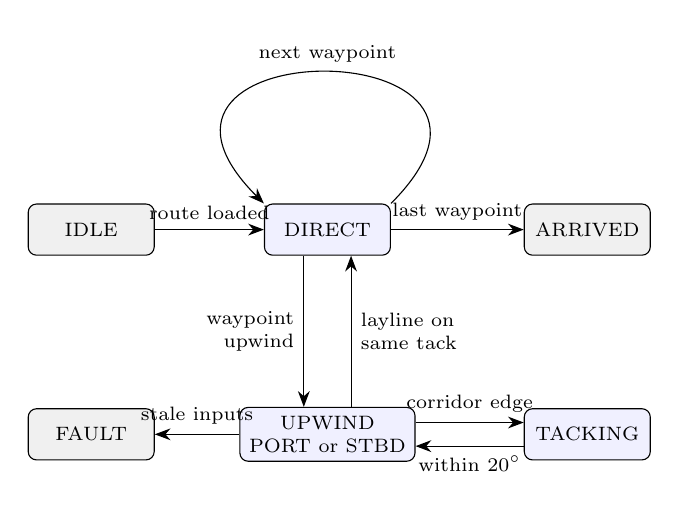
\begin{tikzpicture}[
  font=\scriptsize, >={Stealth[length=2mm]},
  st/.style={draw, rounded corners=3pt, minimum width=16mm, minimum height=6.5mm, align=center, fill=blue!6},
  en/.style={draw, rounded corners=3pt, minimum width=16mm, minimum height=6.5mm, align=center, fill=gray!12}
]
\node[en] (idle) at (0,0)      {IDLE};
\node[st] (dir)  at (3.0,0)    {DIRECT};
\node[en] (arr)  at (6.3,0)    {ARRIVED};
\node[st] (up)   at (3.0,-2.6) {UPWIND\\PORT or STBD};
\node[st] (tk)   at (6.3,-2.6) {TACKING};
\node[en] (flt)  at (0,-2.6)   {FAULT};
\draw[->] (idle) -- node[above]{route loaded} (dir);
\draw[->] (dir) -- node[above]{last waypoint} (arr);
\draw[->] ([xshift=-3mm]dir.south) -- node[left,align=right]{waypoint\\upwind} ([xshift=-3mm]up.north);
\draw[->] ([xshift=3mm]up.north) -- node[right,align=left]{layline on\\same tack} ([xshift=3mm]dir.north |- dir.south);
\draw[->] ([yshift=1.5mm]up.east) -- node[above]{corridor edge} ([yshift=1.5mm]tk.west);
\draw[->] ([yshift=-1.5mm]tk.west) -- node[below]{within \SI{20}{\degree}} ([yshift=-1.5mm]up.east);
\draw[->] (up) -- node[above]{stale inputs} (flt);
\draw[->] (dir.north east) to[out=45,in=135,looseness=5] node[above]{next waypoint} (dir.north west);
\end{tikzpicture}
\caption{Live tack planner states. A fault (stale inputs, too little wind
history, or leaving the corridor) can occur from any sailing state, and
ARRIVED or a corridor fault puts the boat in SAFE.}
\label{fig:fsm}
\end{figure}

\subsection{Telemetry}
The telemetry task packs a 73-byte record into SRAM4 once per second. The
record contains pack and cell voltages; encoder angle, magnetic field
strength, and status; apparent wind angle; GPS position, altitude, satellite
count, fix quality, and time; IMU calibration state and temperature; fused
heading, roll, and pitch; both servo angles as actually driven after clamping
and slew limiting; the mode, desired heading, active leg, and cross-track
distance; the last command's sequence number and result; and uptime. Each
sensor group carries a validity byte. On each TIM6 tick the CM4 copies the
record, retrying about \SI{1}{\milli\second} later if the CM7 is mid-write,
prepends a five-byte header (destination, source, sequence number, length,
and status flags), and transmits the 78-byte frame. Commands from the ground
station use the same header with a payload of up to 16 bytes.

\subsection{Ground Station}
The ground station radio is a SparkFun SAMD21 Pro RF board running a
transparent bridge. Bytes arriving from the laptop over USB are collected
until the line has been idle for \SI{10}{\milli\second} and then sent as one
LoRa packet. Every packet received is written back to USB byte for byte. The
bridge uses the same radio settings as the boat (SF8, \SI{125}{\kilo\hertz},
CR 4/5, \SI{17}{dBm}). All protocol logic runs on the laptop, in three
programs:
\begin{itemize}
\item \texttt{gs\_term}, a terminal program in C. It validates each telemetry
frame's addresses and length and redraws a text status screen. It sends
typed commands for modes, heading and sail-angle targets, and direct servo
angles, and a heartbeat every second. It logs every raw byte with a
timestamp.
\item \texttt{gs\_web}, a browser dashboard written with only the Python
standard library. It reads the telemetry layout from the same C header at
startup, so the firmware structure stays the single definition of the
packet.
\item \texttt{plot\_log}, which converts a session log into CSV files,
twelve plots, and an HTML summary. It decodes the raw radio bytes rather than
the terminal's decoded text, so the plots show exactly what was received. The
field-test figures in Section~\ref{sec:test} were produced with it.
\end{itemize}
A simulated CM4 and bridge on a pseudo-terminal lets the ground station
software be tested without the boat.

Both radios are half duplex, which shaped the command timing. The bridge
cannot read its serial port while it transmits (about \SI{70}{\milli\second}
for a 7-byte command), so the terminal spaces packets at least
\SI{150}{\milli\second} apart. The boat cannot receive while it sends its
\SI{246}{\milli\second} telemetry frame. The team measured that any command
sent between 87 and \SI{347}{\milli\second} before a telemetry packet arrives
is lost. The terminal therefore predicts the next arrival from the boat's
measured \SI{0.997}{\second} telemetry period and holds any command that
would fall in that window.

\section{Testing and Demonstration}
\label{sec:test}

Testing moved from host code to emulated hardware, then to the bench, and
finally to the water, so that each layer was checked before the next depended
on it. Table~\ref{tab:tests} summarizes the tests and their outcomes.

\subsection{Unit Tests}
The route manager, geometry library, and tack planner are compiled with the host C compiler
and exercised by a test harness: CRC values, waypoint validation, incomplete
and corrupted uploads, angle wrapping, bearings, track distances, and circular
means. The tack planner adds tests for every state transition, corridor
and layline tacks, arrival, stale inputs, and wind wrap-around. On the
\texttt{ltp} branch (commit \texttt{ca2e48e}), all 1275 checks pass: 68
geometry, 266 route, and 941 tack-planner checks.

\subsection{Firmware-in-the-Loop Simulation}
Fig.~\ref{fig:sim} shows the simulator the team built to develop control
logic before water time was available. The unmodified CM7 firmware runs on an
emulated STM32H755 in the Renode framework~\cite{renode}. Each sensor is
emulated at the bus level: BNO055 and AS5600 registers over
I\textsuperscript{2}C, the wind vane's Modbus replies over UART, and NMEA
sentences from the GPS. The real drivers therefore run without changes. A
lockstep bridge passes the firmware's servo pulse widths to a Python physics
model of the boat, which returns sensor values. The model is built from the
CAD exports. It takes wing, tail, keel, and rudder areas and the pivot
locations from the geometry, computes buoyancy and righting moment from a
voxel model of the hull and keel, and takes mass and center of gravity from an
editable mass list. It adds wind gusts and shifts, water current, wind-vane
position effects, sensor noise, and the $\pm\SI{90}{\degree}$ wing stops. A
browser dashboard shows the boat in 3D and provides tabs for live sailing,
a bench setup with a fan, route planning, stability curves, and a
points-of-sail polar. Sensors can be failed on command to test the fallback
logic.

The simulator does not yet emulate the CM4 or the radio. Heel is
quasi-static, and hull drag and the tail-to-angle-of-attack gain are estimates
to be calibrated from water tests. It is therefore used to develop and
debug logic, while gains are tuned on the water.

\begin{figure}[!t]
\centering
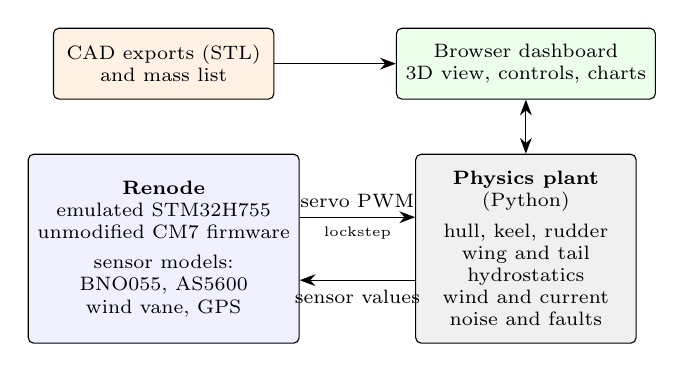
\begin{tikzpicture}[font=\scriptsize, >={Stealth[length=2mm]},
  bx/.style={draw, rounded corners=2pt, align=center, minimum width=28mm, minimum height=9mm}]
\node[bx, fill=blue!6, minimum height=24mm] (ren) at (0,0) {\textbf{Renode}\\emulated STM32H755\\unmodified CM7 firmware\\[3pt]sensor models:\\BNO055, AS5600\\wind vane, GPS};
\node[bx, fill=gray!12, minimum height=24mm] (pl) at (4.6,0) {\textbf{Physics plant}\\(Python)\\[3pt]hull, keel, rudder\\wing and tail\\hydrostatics\\wind and current\\noise and faults};
\node[bx, fill=green!8] (dash) at (4.6,2.35) {Browser dashboard\\3D view, controls, charts};
\draw[->] ([yshift=4mm]ren.east) -- node[above]{servo PWM} node[below,font=\tiny]{lockstep} ([yshift=4mm]pl.west);
\draw[<-] ([yshift=-4mm]ren.east) -- node[below]{sensor values} ([yshift=-4mm]pl.west);
\draw[<->] (dash) -- (pl);
\node[bx, fill=orange!10] (cad) at (0,2.35) {CAD exports (STL)\\and mass list};
\draw[->] (cad) -- (dash.west);
\end{tikzpicture}
\caption{Firmware-in-the-loop simulator. The flight firmware runs unchanged on
an emulated microcontroller and sails a physics model built from the CAD.}
\label{fig:sim}
\end{figure}

\subsection{Bench Tests}
The firmware includes several bench tools that are compiled in only when
needed. A serial console on the ST-LINK USB port, together with a host script
that works with both the real and the emulated board, moves each servo, sweeps
it through its range, and reports status. A dummy-telemetry mode transmits a
fixed packet of recognizable values so that decoding at the ground station
can be checked by eye. A fake-command mode feeds a scripted command list
through the same parse path as received packets, and a commander self-test
steps through every mode at boot. A command stress test sends a long burst
of commands through the inter-core ring. A debug console reports each task's
remaining stack and the share of time the RTOS spends busy, and a fault handler
reports the cause and location of a crash over the serial port. These tools found several faults before the boat reached the water.
\begin{itemize}
\item \emph{Servos.} Both servos map $\pm\SI{90}{\degree}$ to 500 to
\SI{2500}{\micro\second} pulses, centered at \SI{1500}{\micro\second}, and
the arbiters clamp each command to that range. Before the field test, the
team found and fixed a fault in which the rudder arbiter reversed the
commanded direction; on the water, the rudder then followed manual commands
from $+80$ to $-\SI{70}{\degree}$.
\item \emph{Sensors.} Each driver was brought up on the bench before
integration. The sail-angle encoder's range check compared raw counts
against \SI{360}{\degree} and rejected valid readings until it was
corrected. The battery taps were moved off pin PA1, which the Nucleo
board ties to the Ethernet clock (Section~\ref{sec:elec}).
\item \emph{Radio link.} Telemetry first failed to reach the ground
station because the sensor polling tasks starved the telemetry task, so no
packet was ever copied into shared memory. Raising the telemetry task's
priority fixed it. A second fault on the CM4 discarded received commands
whenever a packet was sent, which was fixed by handling reception before
transmission. The half-duplex timing window described in
Section~\ref{sec:sw} was also measured on the bench.
\end{itemize}

\subsection{Field Test}
\label{sec:field}
The first on-water test took place on November 18, 2026, from 16:02 to 16:25,
on Decker Lake pond in the Salt Lake Valley. The operator steered by
sending heading targets in SEMI\_RUDDER\_AUTO\_SAIL mode, so the heading PID,
sail planner, and sail PID were all closed-loop, and finished with manual
rudder in AUTO\_SAIL\_MAN\_RUDDER. The tack planner was not on board.
The link-loss timeout was disabled; it is compiled out on both \texttt{master}
and \texttt{ltp}. The firmware from \texttt{master} was used for this test. Every packet was logged at the ground station. The wind came from
about \SI{294}{\degree} (west-northwest), taken as the circular mean of
heading plus apparent wind angle over the water portion. Wind speed was not
measured on board; the National Oceanic and Atmospheric Administration (NOAA) wind report gave gusts of up to \SI{15}{mph}
(\SI{6.7}{\meter\per\second}), and the water was calm.

Fig.~\ref{fig:field_track} shows the track. From 16:02 to 16:09 the boat
was wheeled to the launch point on its cart, so the track follows the
shoreline footpath and the IMU shows almost no roll. After launch at about 16:09:30, the boat spent
\SI{15.9}{\minute} on the water. It covered \SI{375}{\meter} along its track
and reached \SI{228}{\meter} from the launch point, at a median speed of
\SI{0.35}{\meter\per\second} (peak \SI{0.77}{\meter\per\second}) over
30-second windows.

\begin{figure}[!t]
\centering
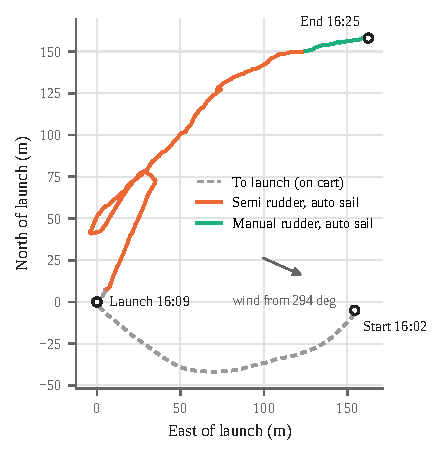
\includegraphics[width=\columnwidth]{field_track}
\caption{GPS track from the November 18 field test, in meters from the launch
point. The dashed segment is the walk to the launch point on the cart; the boat
sailed the solid segments, first with heading targets (semi rudder) and then
with manual rudder, with the sail on auto throughout.}
\label{fig:field_track}
\end{figure}

\paragraph*{Heading control}
Fig.~\ref{fig:field_heading} shows the heading, its target, and the rudder
angle, and Table~\ref{tab:field_heading} summarizes each target held for
longer than \SI{20}{\second}. Error statistics exclude the first
\SI{20}{\second} after each new target. Three behaviors stand out.
\begin{enumerate}
\item On every target at least \SI{49}{\degree} from the wind, the heading
PID held the target with a mean absolute error (MAE) of 3.8 to \SI{8.2}{\degree},
and the rudder was at its \SI{35}{\degree} limit no more than 12\% of the
time.
\item On the two targets inside the no-go zone (\SI{290}{\degree} and
\SI{302}{\degree}, within \SI{6}{\degree} of the wind), the boat settled 42 to
\SI{46}{\degree} off the wind with the rudder at its limit about 90\% of the
time. This measures the boat's closest pointing angle, and it agrees with the
\SI{45}{\degree} no-go angle assumed by the tack planner.
\item At 16:16:50 the boat, on a heading of about \SI{240}{\degree}, was
given a target of \SI{20}{\degree}. The heading PID turns the short way,
which here was through the wind, and the boat stalled in irons for two
minutes with the rudder at its limit. The heading PID alone cannot tack; the
planner's TACKING state, which turns only between close-hauled headings on
each side, exists for exactly this case. A later target of \SI{150}{\degree},
which required bearing away by about \SI{105}{\degree}, was also not reached
in the \SI{27}{\second} before the next command, despite full rudder.
\end{enumerate}

\begin{table}[!t]
\caption{Heading Hold in the Field Test (Wind from About 294$^\circ$)}
\label{tab:field_heading}
\centering
\footnotesize
\begin{tabular}{@{}lrrrrr@{}}
\toprule
Start & Target & Off wind & Held & MAE & Rudder at \\
      & (deg)  & (deg)    & (s)  & (deg) & limit \\
\midrule
16:10:22 & 200 & 90  & 111 & 5.7   & 0\% \\
16:12:26 & 20  & 83  & 90  & 3.8   & 2\% \\
16:14:06 & 200 & 93  & 25  & 4.4   & 12\% \\
16:14:32 & 245 & 49  & 78  & 8.2   & 1\% \\
16:15:50 & 290 & 6   & 32  & 37.5  & 88\% \\
16:16:23 & 200 & 91  & 26  & 22.4  & 44\% \\
16:16:50 & 20  & 97  & 122 & 142.4 & 99\% \\
16:18:53 & 200 & 98  & 44  & 65.2  & 50\% \\
16:19:38 & 150 & 160 & 27  & 108.8 & 100\% \\
16:20:06 & 302 & 2   & 131 & 43.5  & 90\% \\
\bottomrule
\end{tabular}
\end{table}

\begin{figure}[!t]
\centering
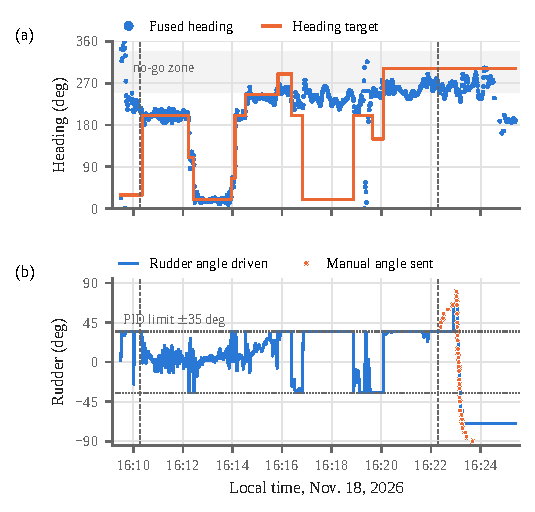
\includegraphics[width=\columnwidth]{field_heading}
\caption{Field test heading control, from launch. (a) Fused heading and heading
PID target; the shaded band is the no-go zone around the
\SI{294}{\degree} wind. (b) Rudder angle driven by the boat, with the PID's
$\pm\SI{35}{\degree}$ limit, and the manual angles sent during the final
sweep. Dashed lines mark the switch to semi rudder (16:10:16) and to manual
rudder (16:22:18).}
\label{fig:field_heading}
\end{figure}

\begin{figure}[!t]
\centering
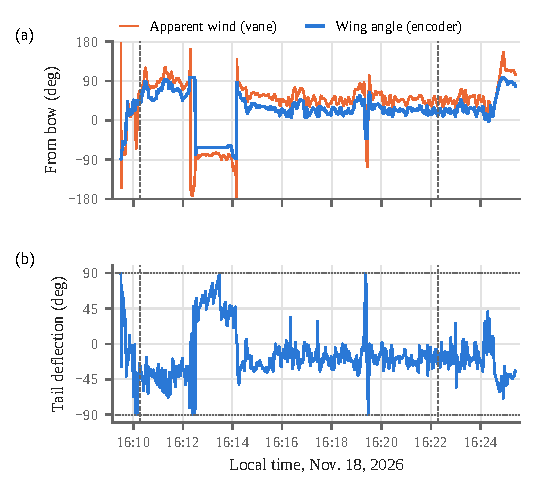
\includegraphics[width=\columnwidth]{field_sail}
\caption{Field test sail control. (a) Apparent wind angle from the vane and
wing angle from the AS5600 encoder, both relative to the bow; the gap between
them is the angle of attack. (b) Tail deflection commanded by the sail PID,
with its $\pm\SI{90}{\degree}$ limits. Dashed lines mark mode changes as in
Fig.~\ref{fig:field_heading}.}
\label{fig:field_sail}
\end{figure}

\paragraph*{Sail control}
Fig.~\ref{fig:field_sail} shows the wing angle following the apparent wind
with an offset, which is the angle of attack. Telemetry does not carry the
sail planner's target, so the target was recomputed from the logged wind
angle with~\eqref{eq:lsp} and Table~\ref{tab:lsp}. In the auto-sail modes on
the water, the wing angle stayed within \SI{10}{\degree} of the target half of
the time and within \SI{23}{\degree} 90\% of the time. Part of that error
comes from the planner's \SI{3}{\degree} deadband and the vane's averaging
window. The median angle of attack was \SI{24}{\degree}, and the tail
reached its $\pm\SI{90}{\degree}$ limit only 2\% of the time, so the
self-trimming wing could be steered with tail authority to spare.

\paragraph*{Stability, radio, and power}
The median heel on the water was \SI{13}{\degree}, the 95th percentile
\SI{29}{\degree}, and the single largest \SI{60}{\degree} at about 16:19:20,
after which the boat righted itself (Fig.~\ref{fig:field_roll}(a)). Pitch
stayed within a few degrees. The ground station received 1296 telemetry
packets and missed 55 (4.1\%), counted from sequence-number gaps. Most losses
fell in the final \SI{90}{\second}, near the far shore
(Fig.~\ref{fig:field_roll}(b)). Of the 65 commands sent, 29 were confirmed, one was
correctly refused (a heading target sent while the rudder was in AUTO), and 8,
all in the final \SI{90}{\second}, were never acknowledged. The remaining 27
were superseded before their result could be reported. Telemetry carries only
the latest command's result once per second, while the manual rudder sweep
sent commands about every \SI{0.3}{\second}. The GPS tracked 10 to 12
satellites with a differential fix the whole time on the water. The pack fell
from \SI{15.97}{\volt} to \SI{15.77}{\volt} over \SI{22.5}{\minute}. The
individual cell readings, however, varied with a standard deviation of about
\SI{180}{\milli\volt}, against \SI{74}{\milli\volt} for the pack, because
subtracting adjacent taps adds their noise.

\begin{figure}[!t]
\centering
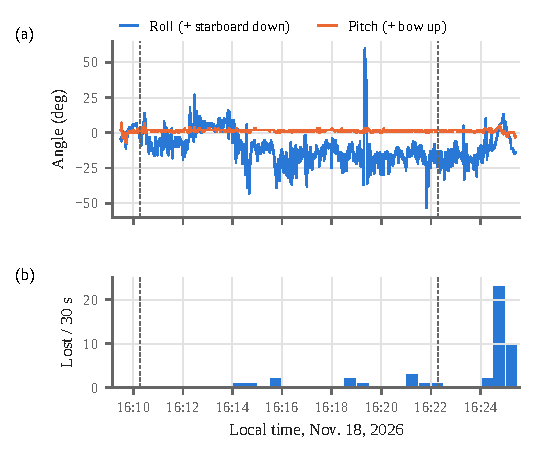
\includegraphics[width=\columnwidth]{field_roll_link}
\caption{Field test stability and radio link. (a) Roll (heel) and pitch from
the BNO055. (b) Telemetry packets lost in each 30-second bin, counted from
sequence-number gaps.}
\label{fig:field_roll}
\end{figure}

\begin{table}[!t]
\caption{Test Plan and Results}
\label{tab:tests}
\centering
\footnotesize
\begin{tabular}{@{}p{0.27\columnwidth}p{0.31\columnwidth}p{0.3\columnwidth}@{}}
\toprule
Test & Pass criterion & Result \\
\midrule
Navigation unit tests & All checks pass & 1275 of 1275 pass (\texttt{ltp} branch) \\
Firmware in the loop & Holds sail target in simulated gusts & Pass \\
Dummy telemetry & Ground station decodes every field & Pass \\
Hull leak test & No water inside after the field test & Pass \\
Float and trim & Level at design waterline & Pass \\
Radio link on water & Telemetry delivered to the far shore & 95.9\% of packets to \SI{228}{\meter} from launch \\
Sail loop & Wing angle follows planner target & Median error \SI{10}{\degree}, 90th percentile \SI{23}{\degree} \\
Manual rudder & Rudder follows ground-station angle & Swept $+80$ to $-70$ deg on command \\
Heading hold & Holds reachable targets & MAE 3.8--\SI{8.2}{\degree} at $\geq$\SI{49}{\degree} off wind \\
Turn through the wind & Reaches a target across the wind & Fail: stalled in irons; needs the tack planner \\
Waypoint course & All waypoints reached & Untested \\
Endurance & ~5-6 hours on one charge & \SI{0.2}{\volt} drop in \SI{22.5}{\minute}; full run untested \\
\bottomrule
\end{tabular}
\end{table}

\subsection{Demonstration}
The final demonstration is autonomous navigation of a waypoint route,
recorded on open water and shown by video at Demo Day.

\section{Safety, Global, Societal, and Ethical Considerations}
\label{sec:impact}

\begin{table*}[!t]
\caption{Risks: Planned Mitigation and Outcome}
\label{tab:risks}
\centering
\footnotesize
\begin{tabular}{@{}p{0.15\textwidth}p{0.33\textwidth}p{0.45\textwidth}@{}}
\toprule
Risk & Planned mitigation (ECE 3992) & Outcome \\
\midrule
\multicolumn{3}{@{}l}{\emph{Mechanical}} \\
Hull integrity failure & Seven fiberglass plies, reinforced keel mount and stern, submersion test & Seven plies with reinforced keel boss and transom; leak test passed with no water inside \\
Keel detachment & Stainless bracket, bolts with lock nuts, embedded plate & 304 bracket bolted through the reinforced boss with nylon-insert lock nuts; zinc-plated fasteners corroding, to be replaced \\
Rudder bearing seizure & R188 ceramic bearings, marine grease, field-replaceable & Ceramic bearings in a removable two-part clamp \\
Mast or sail damage & Design margin; self-trimming wing feathers in gusts & Wing weathervanes freely; $\pm\SI{90}{\degree}$ stops protect the mast cable; high-wind check passed: the keel righted the boat after hard pushes and in field-test gusts \\
\midrule
\multicolumn{3}{@{}l}{\emph{Electrical}} \\
Water ingress & Sealed Pelican case, IP-rated pass-throughs, conformal coating & Printed enclosure under a latched hatch, cable glands, sealed SMA bulkhead and vane connector; breadboard not yet coated (open) \\
Battery failure & BMS & Per-cell voltage telemetry from four ADC taps; BMS fitted \\
LoRa link loss & \SI{10}{dBi} antennas, return to home, mission stored on board & Masthead \SI{10}{dBi} antenna; route stored on board with CRC; 95.9\% packet delivery to \SI{228}{\meter} in the field test; link-loss timeout implemented but off by default; return to home not implemented (open) \\
Servo failure & Waterproof 20 kg-cm servos, stall current monitoring & DS3218MG rudder servo; PID output limits and \SI{120}{\degree\per\second} slew limit; current monitoring not implemented \\
\midrule
\multicolumn{3}{@{}l}{\emph{Software}} \\
Sensor fusion divergence & Complementary filter, range checks, GPS-only fallback & BNO055 onboard fusion; every reading carries a validity code and staleness timeout; the heading PID stops when orientation data are unavailable \\
Real-time deadline miss & Task priorities, execution profiling, dual-core split & Radio moved to the CM4; fixed-rate tasks with consequence-ordered priorities \\
Path-planning edge cases & Tacking state machine, simulation before water trials & Tack planner implemented with 941 unit-test checks and a simulator route mode; not yet sailed on the water \\
No viable path & Planning timeout, loiter, then return to home & Corridor fault and arrival put the boat in SAFE; loiter and return to home not implemented (open) \\
\midrule
\multicolumn{3}{@{}l}{\emph{Found during development}} \\
Mismatched core firmware & -- & Shared-memory layout version checked at boot; CM4 refuses to attach on mismatch \\
Angle averaging at the seam & -- & Unwrapped running averages for encoder and vane; circular mean in navigation \\
\bottomrule
\end{tabular}
\end{table*}


\subsection{Public Health, Safety, and Welfare}
ALAN operates on open water near other watercraft, swimmers, and wildlife.
It is small (\SI{1}{\meter}, about \SI{5}{\kilo\gram}) and wind-powered, so
its speed and the energy of any collision are low. Testing is limited to
small, controlled bodies of water with an operator in sight, and the boat
reports its GPS position every second so it can always be located. The
operator can take control at any time with a mode command, and the SAFE mode
centers the rudder and feathers the tail. Within the firmware, each actuator
has a single writer with a timeout: if a controller crashes or is starved, the
rudder centers within \SI{200}{\milli\second} and the tail returns to its
safe angle within \SI{300}{\milli\second}. The link-loss timeout that drops
manual and semi-autonomous modes to SAFE is implemented but disabled for bench
work. It must be enabled before any unattended run. The 4S LiPo battery is the
main hazard on board; per-cell voltages are reported in every telemetry
packet so a weak or over-discharged cell is visible from shore.
The pack is fitted with a BMS and is charged with a professional battery
charger. Between uses it is unplugged completely from the circuit and left to
sit.

\subsection{Environmental Factors}
Wind propulsion produces no emissions and no underwater noise, and the battery
powers only the electronics. The hull is sealed fiberglass and epoxy, and the
keel and rudder hardware is stainless steel. Zinc-plated fasteners on the keel
are already corroding and will be replaced, so that no coating or rust
residue enters the water. A lost vessel would become debris, which is a
further reason for continuous position telemetry.

\subsection{Global and Cultural Factors}
Low-cost autonomous sailing platforms could make marine research more
accessible, particularly for coastal nations and institutions with limited
research budgets. The same technology could be misused, for example for
smuggling or for operation in protected marine areas without authorization.
Responsible deployment requires operating only where permitted.

\subsection{Economic Factors}
ALAN was built for roughly \$1000 from development boards, commodity sensors,
and fabrication resources available to most universities, a small fraction
of the cost of a commercial uncrewed sailing vessel. The firmware, simulator,
and design files are kept in a shared repository so other teams can build on
them.

\subsection{Professional and Regulatory Obligations}
Engineers have an obligation to ensure the vessel cannot harm people or the
environment, which motivates the failsafe behavior above, clear marking of
the boat as uncrewed, and operation only in permitted waterways. The radio
uses the unlicensed 902--928 MHz band, where Section 15.247 of the Federal Communications Commission (FCC) rules
covers only frequency-hopping and digitally modulated transmitters. In this
band, a hopping system with a channel narrower than \SI{250}{\kilo\hertz}
must use at least 50 frequencies and dwell no more than \SI{0.4}{\second} on
any one in \SI{20}{\second}, and a digitally modulated system must have a
bandwidth of at least \SI{500}{\kilo\hertz}~\cite{cfr15247}. ALAN currently
transmits on a single fixed \SI{125}{\kilo\hertz} channel for about
\SI{246}{\milli\second} every second, so it meets neither condition at its
present \SI{17}{dBm} output. Before further field use, the team should either
add frequency hopping across the band or reduce power to the limits for
non-hopping transmitters. Neither change has been made yet,
and the November 18 field test used the single-channel configuration.
Frequency hopping is the preferred option because it keeps the present range.
The SX1276 includes a hopping mode that changes channel on a programmable
period~\cite{sx1276}, and the ground-station radio would need to follow the
same channel sequence. This change is listed in Section~\ref{sec:future}.
\section{Risks and Mitigations}
\label{sec:risks}

\begin{figure*}[!t]
\centering
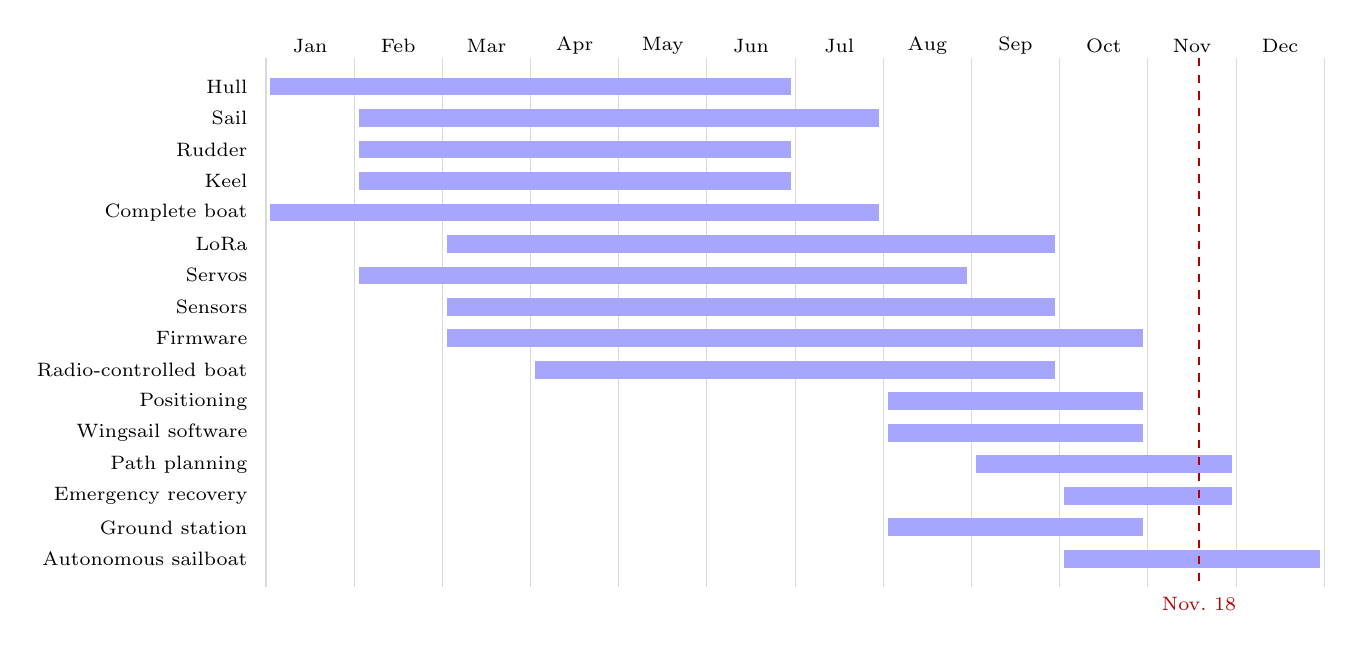
\begin{tikzpicture}[font=\scriptsize, x=1.12cm, y=-0.40cm]
  \foreach \m [count=\i] in {Jan,Feb,Mar,Apr,May,Jun,Jul,Aug,Sep,Oct,Nov,Dec} {
    \node at (\i-0.5,-0.9) {\m};
    \draw[gray!30] (\i-1,-0.5) -- (\i-1,16.3);
  }
  \draw[gray!30] (12,-0.5) -- (12,16.3);
  \foreach \t/\a/\b [count=\r from 0] in {
      Hull/1/6, Sail/2/7, Rudder/2/6, Keel/2/6, Complete boat/1/7,
      LoRa/3/9, Servos/2/8, Sensors/3/9, Firmware/3/10, Radio-controlled boat/4/9,
      Positioning/8/10, Wingsail software/8/10, Path planning/9/11,
      Emergency recovery/10/11, Ground station/8/10, Autonomous sailboat/10/12} {
    \node[anchor=east] at (-0.1,\r+0.4) {\t};
    \fill[blue!35] (\a-1+0.05,\r+0.12) rectangle (\b-0.05,\r+0.68);
  }
  \draw[red!70!black, thick, dashed] (10.58,-0.5) -- (10.58,16.3);
  \node[red!70!black, anchor=north] at (10.58,16.3) {Nov.\ 18};
\end{tikzpicture}
\caption{Planned schedule from the ECE 3992 proposal (January to December
2026). The dashed line marks the date of this report.}
\label{fig:gantt}
\end{figure*}

\begin{table*}[!t]
\caption{Milestone Owners and Status}
\label{tab:schedule}
\centering
\footnotesize
\begin{tabular}{@{}>{\raggedright\arraybackslash}p{0.17\textwidth}l>{\raggedright\arraybackslash}p{0.25\textwidth}>{\raggedright\arraybackslash}p{0.42\textwidth}@{}}
\toprule
Milestone & Planned & Owner (proposal) & Status \\
\midrule
Hull                      & Jun 2026 & Harrison LeTourneau & Complete \\
Keel                      & Jun 2026 & Corbin Barney, Jared Pratt & Complete; removable ballast canisters replaced the steel-ball fill \\
Rudder                    & Jun 2026 & Corbin Barney, Jared Pratt & Complete \\
Wingsail                  & Jul 2026 & Charbel Salloum, Connor Stevens & Complete; direct tail drive; bare foam skin, fiberglass planned for the final iteration \\
Complete boat assembly    & Jul 2026 & ALAN team & Assembled and sailed; balance in Section~\ref{sec:integration} \\
Servo control             & Aug 2026 & Sensor team & Complete: arbiters with timeouts and slew limits, console control \\
LoRa communication        & Sep 2026 & LoRa team & Bidirectional with CRC and command results; 95.9\% delivery on Nov.\ 18 \\
Sensor integration        & Sep 2026 & Sensor team & Complete: GPS, IMU, encoder, wind vane, battery \\
Radio-controlled sailboat               & Sep 2026 & ALAN team & Complete: manual and semi modes sailed on Nov.\ 18 \\
Dual-core firmware        & Oct 2026 & Embedded team & Complete: FreeRTOS on CM7, bare-metal radio on CM4 \\
Positioning               & Oct 2026 & Corbin Barney, Harrison LeTourneau & BNO055 fusion with GPS; dead reckoning through GPS dropouts not implemented \\
Wingsail software         & Oct 2026 & Jared Pratt & Sail planner and PID field-tested Nov.\ 18 \\
Ground station interface  & Oct 2026 & Harrison LeTourneau & Complete: terminal, web dashboard, log plotter \\
Path planning             & Nov 2026 & Charbel Salloum & Route manager and tack planner unit-tested and simulated; not yet sailed \\
Emergency recovery        & Nov 2026 & Corbin Barney & SAFE mode and link-loss timeout done; return to home and low-battery response open \\
Autonomous demonstration  & Dec 2026 & ALAN team & Incomplete \\
\bottomrule
\end{tabular}
\end{table*}


The proposal identified twelve risks across the mechanical, electrical, and
software subsystems. Table~\ref{tab:risks} lists each with the planned
mitigation and what was actually done. Two further risks were found during
the fall and are listed at the end. Risks still marked open are carried
into the remaining work in Section~\ref{sec:future}.
\section{Project Management}
\label{sec:mgmt}

\subsection{Team and Responsibilities}
The five team members split into sub-teams by subsystem, and three additional
contributors assisted with the radio and sensors.
Table~\ref{tab:team} lists each member's responsibilities, taken from the
proposal schedule and the fall firmware task plan. The proposal organized the work into four sub-teams:
\begin{itemize}
\item \emph{LoRa}: Harrison LeTourneau, Jared Pratt, Adam Welsh, and Aliou
Tippett designed, implemented, and tested the radio link between the vessel
and the ground station.
\item \emph{Sensor}: Corbin Barney, Charbel Salloum, Connor Stevens, and
Derek Tinoco selected, integrated, and tested the GPS, IMU, and wind vane.
\item \emph{Embedded}: all five members, with Derek Tinoco, Adam Welsh, and
Aliou Tippett, built the bench test setups for the radio and sensor suite.
\item \emph{ALAN}: the five members shared vessel integration, mechanical
assembly, firmware integration, and on-water testing.
\end{itemize}
Adam Welsh and Aliou Tippett are students at the University of Utah, and
Derek Tinoco is a computer scientist who assisted with early sensor
integration.

\begin{table}[!htb]
\caption{Team Responsibilities}
\label{tab:team}
\centering
\footnotesize
\begin{tabular}{@{}p{0.22\columnwidth}p{0.3\columnwidth}p{0.38\columnwidth}@{}}
\toprule
Member & Mechanical & Firmware and software \\
\midrule
Charbel Salloum & Wingsail & Wingsail control, live tack planner, path planning \\
Connor Stevens & Wingsail & Wingsail control, telemetry \\
Corbin Barney & Keel, rudder & Sensor drivers, shared data types, positioning, emergency recovery \\
Harrison LeTourneau & Hull & LoRa link (CM4), commander, positioning, ground station \\
Jared Pratt & Keel, rudder & Heading and sail PIDs, arbiters, sail planner, ground station, path planning \\
\bottomrule
\end{tabular}
\end{table}

\subsection{Schedule}
Fig.~\ref{fig:gantt} shows the schedule planned in the proposal. The spring
and summer covered fabrication and assembly, and the fall covered firmware,
control, navigation, and water testing. Table~\ref{tab:schedule} gives the
owner assigned in the proposal and the status of each milestone at the time
of writing.

\subsection{Cost}
The proposal estimated a total of about \$1000, shown against actual
spending in Table~\ref{tab:cost}. The largest single expense was expected to be
epoxy resin, and the most expensive component the hull, because of the
printed mold and its filament. On-campus groups sponsored some materials,
including 3D printing filament, and university staff loaned reusable
equipment such as respirators. John Davies provided a space in the ECE Senior Capstone Lab to house materials and a space to assemble the project.

\begin{table}[!htb]
\caption{Estimated and Actual Cost}
\label{tab:cost}
\centering
\begin{tabular}{@{}lrr@{}}
\toprule
Category & Estimate (\$) & Actual (\$) \\
\midrule
Hull materials (resin, fiberglass, mold) & 400 & 375 \\
Keel, rudder, sail/tail (steel, carbon fiber, etc.)    & 200 & 145 \\
Electronics                              & 200 & 250 \\
Contingency                              & 200 & 250 \\
\midrule
Total                                    & 1000 &  1020\\
\bottomrule
\end{tabular}
\end{table}
\section{Remaining Work}
\label{sec:future}

To finish the capstone vessel, the team must complete the following:
\begin{itemize}
\item Merge the \texttt{ltp} branch into \texttt{master} and sail the test
route on the water. The field test showed that the heading PID alone stalls when a
turn passes through the wind.
\item Enable the link-loss timeout and confirm the safe tail angle before
unattended operation.
\item Bring the radio link into compliance with FCC Part~15, by adding
frequency hopping or reducing output power (Section~\ref{sec:impact}).
\item Report each command's result individually, for example as a short
history in telemetry. In the field test, 27 of 65 command results were
overwritten before the ground station could see them.
\item Find the cause of the restart at 16:04:18 in the field test.
\item Confirm on the water that the \texttt{ltp} firmware's longer battery
window (20 readings instead of 2) removes the cell-voltage noise seen in the
field test, where individual cells varied by about \SI{180}{\milli\volt}
between packets.
\item Calibrate the simulator's hull drag and tail-to-angle-of-attack gain
from the field-test log, then retune both PIDs and the sail-planner table.
\item Run the full waypoint mission and record the data for
Section~\ref{sec:test}.
\end{itemize}
Before any longer deployment, the following changes are recommended:
\begin{itemize}
\item Replace the solderless breadboard with soldered connections.
\item Replace zinc-plated fasteners on the keel with stainless hardware.
\item Test the monohull's stability in rough water, and add outriggers if the
keel alone does not keep heel within limits.
\item Emulate the CM4 and radio in the simulator so the full command path can
be tested off the water.
\item Add an energy source, such as a solar panel, and use the cell-voltage
telemetry to manage energy on long missions.
\item Add obstacle avoidance and weather routing~\cite{stelzer2012}.
\end{itemize}
\section{Conclusion}
\label{sec:conclusion}

ALAN is a wind-propelled sailboat built to carry out waypoint missions with
little energy beyond what its sensors and radio require. The team built a
fiberglass displacement hull from a printed mold, a 304 stainless keel with
adjustable ballast canisters, a servo-driven spade rudder, and a
self-trimming wingsail whose tail is driven directly by a small servo. The
firmware divides the STM32H755's two cores by timing requirement: the CM7 runs
sensing, sail planning, PID control, and eleven operating modes under
FreeRTOS, and the CM4 runs the LoRa link. The cores share data through a
versioned, lock-free shared-memory interface. Single-writer arbiters with
timeouts keep each actuator safe if a controller stalls, and a
firmware-in-the-loop simulator built from the CAD let the team develop the
control logic before water time was available. In its first field test the
boat sailed \SI{375}{\meter} under semi-autonomous control and held
reachable headings within 4 to \SI{8}{\degree}, while the self-trimming wing
followed the wind with tail authority to spare. The boat pointed within
\SI{42}{\degree} to \SI{46}{\degree} of the wind, and the radio delivered
95.9\% of packets. The same test confirmed the limits that the remaining
work addresses: without the tack planner, the boat cannot turn through the
wind, and the command acknowledgment scheme loses results during rapid
command sequences.


% ===========================================================================
\appendices
\section{Bill of Materials}
\label{app:bom}
Tables~\ref{tab:bom_mech} and~\ref{tab:bom_elec} list the materials and
components in the vessel as built. Consumables such as brushes, mixing cups,
sandpaper, and personal protective equipment are omitted.

\begin{table*}[!t]
\caption{Bill of Materials: Mechanical}
\label{tab:bom_mech}
\centering
\footnotesize
\begin{tabular}{@{}p{0.12\textwidth}p{0.36\textwidth}p{0.45\textwidth}@{}}
\toprule
Subsystem & Item & Specification or note \\
\midrule
Hull & PLA filament (mold) & Two-piece female mold, lab provided \\
     & Filler primer, 2K gloss topcoat & Mold surface finish \\
     & PARTALL \#2 paste wax, PARTALL \#10 PVA & Mold release \\
     & Fiberglass cloth & \SI{4}{oz} plain weave, \SI{50}{in} wide, seven plies \\
     & TotalBoat 5:1 marine epoxy, peel ply & Layup \\
     & XPS foam board & Deck; laminated with fiberglass \\
     & Plywood & Laser-cut bulkheads and sail templates \\
     & Printed hatch coamings and latches & Two hatches, four over-center latches each \\
Keel & 304 SS square bar & \SI{0.5}{in} $\times$ \SI{7}{in} post \\
     & 304 SS plate & \SI{0.25}{in} mounting bracket \\
     & 304 SS round tube & \SI{2}{in} $\times$ \SI{8.5}{in} bulb core \\
     & Ballast canisters & Stainless tubes with threaded studs, printed nose and tail caps \\
     & PLA fairing halves & Mirrored, bolted around the post \\
     & 1/4-20 bolts, nylon-insert lock nuts, washers & Bracket mounting; replace zinc-plated bolts \\
Rudder & 304 SS round bar & \SI{0.25}{in} $\times$ \SI{12}{in} shaft \\
       & R188 ceramic bearings (2) & $1/4 \times 1/2 \times 3/16$ in \\
       & Aluminum plates & \SI{0.065}{in}, rear clamp \\
       & Printed blade, cross bolt and barrel nut & Swappable blade \\
       & 25-tooth spline to 1/4-in.\ coupler & Servo to shaft \\
Wingsail & 6061 aluminum tube & \SI{3}{ft} mast \\
         & Flanged ball-bearing unit & Deck mast partner \\
         & XPS foam board & Main wing and tail \\
         & Carbon fiber rods & Tail and counterweight booms \\
         & Printed parts & Collar and stops, tail servo bracket, upper pivot, counterweight \\
\bottomrule
\end{tabular}
\end{table*}

\begin{table*}[!t]
\caption{Bill of Materials: Electrical}
\label{tab:bom_elec}
\centering
\footnotesize
\begin{tabular}{@{}p{0.12\textwidth}p{0.36\textwidth}p{0.45\textwidth}@{}}
\toprule
Subsystem & Item & Specification or note \\
\midrule
Control  & NUCLEO-H755ZI-Q & STM32H755 dual-core development board \\
Sensors  & Adafruit BNO055 breakout & Nine-axis orientation, I\textsuperscript{2}C \\
         & u-blox NEO-6 GPS module & NMEA over UART \\
         & DFRobot wind vane & RS-485 Modbus RTU, aviation connector \\
         & RS-485 to UART adapter & Wind vane interface \\
         & AS5600 magnetic encoder & Sail angle, I\textsuperscript{2}C \\
Actuators & DS3218MG digital servo & 20 kg-cm, waterproof, rudder \\
          & MG90S 9G Servo & Mounted on the lower tail boom \\
Radio    & Adafruit RFM95W breakout & 915 MHz LoRa, boat \\
         & SparkFun SAMD21 Pro RF & Ground station USB-to-LoRa bridge \\
         & \SI{10}{dBi} whip antennas (2) & Boat masthead and ground station \\
         & SMA to u.FL cables, \SI{5}{ft} SMA extension & Antenna feed to masthead \\
         & SMA bulkhead connector & Enclosure pass-through \\
Power    & 4S LiPo battery & \SI{14.8}{\volt} nominal, 1300 mAh \\
         & Power distribution board, XT60 connectors & Servo and logic rails \\
         & 82 k$\Omega$ / 18 k$\Omega$ dividers, 100 nF capacitors & Four cell-tap channels \\
Packaging & Printed enclosure, cable glands & Aft hatch \\
          & Solderless breadboard & Interconnections \\
\bottomrule
\end{tabular}
\end{table*}

\section*{Acknowledgment}
The authors thank Micah Frerck for help with laser cutting the sail
templates and bulkheads; Adam Welsh, Aliou Tippett, and Derek Tinoco for
their work on the radio link and sensor integration; Ken Stevens and Will Taylor for their support throughout the project; and the University of Utah groups that sponsored
materials. As with the ECE 3992 proposal, this report was drafted with the
assistance of an artificial intelligence (AI) tool (Claude Opus 5.5) for writing, editing, and
formatting. The team provided the technical content, design decisions, and
data, and takes full responsibility for the final report.


\IEEEtriggercmd{\enlargethispage{\baselineskip}}
\IEEEtriggeratref{12}
\bibliographystyle{IEEEtran}
\bibliography{references}

\end{document}
